%
% thesis-doc
%
% @version 1.0
% @author wipatrick
% @created 22. November 2015
% @edited 
%
%----------------------------------------------------------------------------------------------------------------------
% Definition
%----------------------------------------------------------------------------------------------------------------------
\documentclass[
11pt, 						                                   % Schriftgröße
oneside, 					                                   % Einseitiges Dokument
a4paper,  				 	                                   % DINA4
BCOR10mm, 					                                   % Kleberand
%nochapterprefix, 			                                   % Zusatz  Kapitel anschalten
%noappendixprefix, 			                                   % Zusatz  beim Anhang abschalten
numbers=noenddot,			                                   % Kein Punkt am Ende der Nummerierung
bibliography=totoc,			                                   % Literaturverzeichnis ins ToC
listof=totoc, 				                                   % Abbildungs- und Tabellenverzeichnis ins ToC
headsepline,				                                   % Linie unter Kopfzeile
parskip,					                                   % Absatz nicht einrücken
listof=nochaptergap			                                   % Kein vertikaler Abstand zw. Abb./Tab. untersch. Kapitel
]{scrreprt}
\usepackage{etex}
\usepackage{scrhack}

%----------------------------------------------------------------------------------------------------------------------
% Präambel
%----------------------------------------------------------------------------------------------------------------------
%
% präambel packages
%
% @version 1.0
% @author wipatrick
% @created 22. November 2015
% @edited  
%
%----------------------------------------------------------------------------------------------------------------------
% Allgemeines
%----------------------------------------------------------------------------------------------------------------------
\usepackage[utf8]{inputenc}
%\DeclareUnicodeCharacter{00A0}{ }
%\DeclareUnicodeCharacter{00A0}{~}
\usepackage[T1]{fontenc}                                         % wichtig für Trennung von Wörtern mit Umlauten
\usepackage{lmodern}
\usepackage{microtype}                                           % verbesserter Randausgleich
\usepackage{url}                                                 % zum Zitieren von url
%\urlstyle{rm}                                                   % Serifenstil für URL im Literaturverzeichnis
%\usepackage[singlelinecheck=false]{caption}                     %justification=RaggedRight, linksbündige 
\usepackage{multirow}
\usepackage{lipsum}
\usepackage{textcomp}                                            % Nummer-Zeichen \textdegree N°
\usepackage{xcolor}                                              % definiert, dass hyperlinks nicht gefärbt sind
\definecolor{black}{gray}{0}                                     % 10% gray
\usepackage[colorlinks=true,linkcolor=black,citecolor=black,urlcolor=black]{hyperref}
\renewcommand*{\theHsection}{\thesection}                        % Anhang richtig verlinkt im InhaltsVZ
\usepackage[ngerman]{babel}                                      % deutsche Trennregeln

%----------------------------------------------------------------------------------------------------------------------
% Radar Chart
%----------------------------------------------------------------------------------------------------------------------
\PassOptionsToPackage{pdf}{pstricks}                             % used for pdflatex
\usepackage{pstricks-add}

\usepackage{dirtree}                                             % Verzeichnisstruktur 
\usepackage{calc}                                                % Listing Nummer Abstand
\usepackage{pifont}                                              % Checkmark

\usepackage{booktabs}
%\usepackage{cite}
\usepackage[square]{natbib}
\setlength{\bibsep}{0.25cm}
\renewcommand{\bibfont}{\small} %\normalsize
\renewcommand*{\bibpreamble}{\interlinepenalty10000\relax}

%----------------------------------------------------------------------------------------------------------------------
% Gänsefüßchen
%----------------------------------------------------------------------------------------------------------------------
\usepackage{xspace}                                              % Gänsefüßchen
\newcommand{\Gun}{\glqq{}}		                                  % Gänsefüßchen unten
\newcommand{\Gob}{\grqq\xspace} 	                                  % Gänsefüßchen oben


%----------------------------------------------------------------------------------------------------------------------
% Layout
%----------------------------------------------------------------------------------------------------------------------
\usepackage[automark]{scrpage2}
\automark[section]{chapter} 
\pagestyle{scrheadings}
\clearscrheadfoot
\ihead{\leftmark}
\ohead{\pagemark}
\renewcommand*{\chapterpagestyle}{scrheadings}
\renewcommand*{\indexpagestyle}{scrheadings}
\usepackage[left=30mm,right=38mm,top=30mm,bottom=20mm]{geometry}
%\addtokomafont{sectioning}{\rmfamily} %Serifenstyle für Section
\renewcommand{\chapterheadstartvskip}{\vspace*{0cm}}
\renewcommand{\chapterheadendvskip}{\vspace*{1.5\baselineskip}}
\setkomafont{chapterprefix}{\large} % Kapitelpräfixgröße
\setkomafont{chapter}{\LARGE} % Kapitelgröße
\setlength{\parskip}{0.5EM} %Paragraphen/Absatzabstand

% Überschriften Serifen-Schriftart 
%\addtokomafont{chapter}{\rmfamily}                               
%\addtokomafont{section}{\rmfamily} 
%\addtokomafont{subsection}{\rmfamily} 
%\addtokomafont{subsubsection}{\rmfamily} 

%----------------------------------------------------------------------------------------------------------------------
% Tabellen- und Abbildungsverzeichnis
%----------------------------------------------------------------------------------------------------------------------
\makeatletter                                                     % Einrücken verhindern
\renewcommand*\l@figure{\@dottedtocline{1}{0em}{2.3em}}           % Default: 1.5em/2.3em
\let\l@table\l@figure
\makeatother

\renewcommand{\thefigure}{Abb. \arabic{chapter}.\arabic{figure}} 
\renewcommand{\thetable}{Tab. \arabic{chapter}.\arabic{table}}
\renewcommand{\theequation}{Gl. \arabic{equation}}
\renewcommand*{\figureformat}{\thefigure} 
\renewcommand*{\tableformat}{\thetable} 
\renewcommand*{\captionformat}{: }  

\addtokomafont{caption}{\small\sffamily}		                   % Bild-/Tabellenunterschriften klein & serifenlos
\addtokomafont{captionlabel}{\sffamily\bfseries}                  % Bild-/Tabelllabel fett & serifenlos

\AtBeginDocument{                                                 % Doppelpunkt nach Nummern 
  \addtocontents{lof}{\protect\def\protect\autodot{:}}% 
  \addtocontents{lot}{\protect\def\protect\autodot{:}}% 
} 

%----------------------------------------------------------------------------------------------------------------------
% Tabellen
%----------------------------------------------------------------------------------------------------------------------
\usepackage{tabularx}
\usepackage{stypackage/stackengine}                                % Pfeile in Tabelle
\usepackage{varwidth}
\usepackage{longtable}                                             % Ermöglicht Tabellen über Seitenumbruch
\usepackage[]{threeparttable}                                      % Fußnoten in Tabellen
\usepackage{booktabs}
\usepackage{pdflscape}
\usepackage{colortbl}
\usepackage{enumitem}                                              % Liste in Tabelle
\usepackage{arydshln}                                              % Dashedlines in Tables
\usepackage{hhline}

\newcommand\Thickvrule[1]{
  \multicolumn{1}{!{\vrule width 1.5pt}l!{\vrule width 1.5pt}}{#1} % vertikaler Strich (1.5) LINKS & RECHTS der Zelle
}
\newcommand\Thickvrulel[1]{
  \multicolumn{1}{!{\vrule width 1.5pt}l}{#1}                      % vertikaler Strich (1.5) LINKS der Zelle
}
\newcommand\Thickvruler[1]{
  \multicolumn{1}{c!{\vrule width 1.5pt}}{#1}                      % vertikaler Strich (1.5) RECHTS der Zelle
}
\newcommand\Thinvrulel[1]{
  \multicolumn{1}{!{\vrule width 0.75pt}l}{#1}                     % vertikaler Strich (0.75) LINKS der Zelle
}
\newcommand\Thinvruler[1]{
  \multicolumn{1}{c!{\vrule width 0.75pt}}{#1}                     % vertikaler Strich (0.75) RECHTS der Zelle
}

\newcommand\stdrulel[1]{
	\multicolumn{1}{!{\vrule}c}{#1}
}
\newcommand\stdruler[1]{
	\multicolumn{1}{c!{\vrule}}{#1}
}
\newcommand\stdrulelinksb[1]{
	\multicolumn{1}{!{\vrule}l!{\vrule}}{#1}
}
\newcommand\stdrulecent[1]{
	\multicolumn{1}{!{\vrule}c!{\vrule}}{#1}
}
\newcommand\stdrulellinks[1]{
	\multicolumn{1}{!{\vrule}l}{#1}
}
\newcommand\stdrulerlinks[1]{
	\multicolumn{1}{l!{\vrule}}{#1}
}

\newcommand\RotText[1]{\rotatebox[origin=c]{90}{\parbox{1cm}{\centering#1}}}


\newcommand{\myitem}{\item\quad}                                  % horizontaler Abstand itemize
\newcommand{\ccol}{\cellcolor{black!20}}                          % CellColor Grau

\def\RA{\rlap{\scalebox{1.6}{$\rightarrow$}}}                     % Pfeile in Tabelle zeichnen stypackage/stackengine
\def\DA{\smash{\bclap{\scalebox{1.6}{$\downarrow$}}}}

\makeatletter                    
\def\hlinewd#1{
\noalign{\ifnum0=`}\fi\hrule \@height #1                         % Dicke der horizontalen Linie
\futurelet\reserved@a\@xhline}
\makeatother

\newcolumntype{Y}{>{\centering\arraybackslash}X}                 % ColumnType


% Entwurfslayout
\newcolumntype{V}[1]{%
  >{\begin{varwidth}[t]{\dimexpr\textwidth-\wd#1-2\fboxsep-2\fboxrule\relax}\arraybackslash}
    l<{\strut\end{varwidth}}}

\newsavebox\Breitestes % Box für längstes „item“
%Syntax: \Rahmen[<trenner>]{<längstes „item“>}{<tabelleninhalt>}
\newcommand\Rahmen[3][:\qquad]{%
  \sbox\Breitestes{#2#1}%
  \begin{flushleft}%
   {\renewcommand{\arraystretch}{1.2}\begin{tabular}{@{}l<{#1}@{}V{\Breitestes}@{}}
      #3
    \end{tabular}}%
  \end{flushleft}
}

%----------------------------------------------------------------------------------------------------------------------
% Abbildungen
%----------------------------------------------------------------------------------------------------------------------
\usepackage{graphicx}                                              % Einbinden von Grafiken mit Pfadangabe
\usepackage{float}                                                 % zum genauen platzieren von Grafiken und Tabellen
\graphicspath{{images/}}
\usepackage{pdfpages}                                              % Einbinden PDF-Dateien


%----------------------------------------------------------------------------------------------------------------------
% Inhaltsverzeichnis
%----------------------------------------------------------------------------------------------------------------------
%\usepackage[nottoc]{tocbibind}
\setcounter{secnumdepth}{3} 
\renewcommand*{\theparagraph}{\thesubsubsection.\alph{paragraph}} 
%\setcounter{secnumdepth}{3}
\setcounter{tocdepth}{3}
% ------ section fett im TOC
\usepackage{tocstyle}
\usetocstyle{allwithdot}
%\usetocstyle{KOMAlike}
\settocfeature[toc][1]{entryhook}{\protect\hspace*{-0.5em}\nobreakspace} % Section Horizontal in InhaltsVZ anpassen an Chapter
\settocfeature[toc][2]{entryhook}{\protect\hspace*{-0.9em}\nobreakspace} % Subsection Horizontal in InhaltsVZ anpassen an Section
\settocfeature[toc][3]{entryhook}{\protect\hspace*{-0.9em}\nobreakspace} % Subsection Horizontal in InhaltsVZ anpassen an Section
%\settocfeature[lof][1]{entryhook}{\protect\hspace*{-1.9em}\nobreakspace} % Kein horizontaler Einzug
%\settocfeature[lof][2]{entryhook}{\protect\hspace*{-1.9em}\nobreakspace} % Kein horizontaler Einzug
%\settocfeature[lot][1]{entryhook}{\protect\hspace*{-1.9em}\nobreakspace}
%\settocfeature[lot][2]{entryhook}{\protect\hspace*{-1.9em}\nobreakspace}


\usepackage{setspace}                                            % 1,5-zeiligen Zeilenabstand
\onehalfspacing 
%\BeforeStartingTOC[toc]{\singlespacing} 

%TIKZ zum Zeichnen
\usepackage{pgfplots}
\usepackage{tikz}
\usetikzlibrary{arrows,calc,positioning}
\usepackage[format=hang]{subfig} %margin=10pt,
%\usepackage{subcaption}
\pgfplotsset{compat=newest}
\usepgfplotslibrary{dateplot}

%----------------------------------------------------------------------------------------------------------------------
% Mathematische Formeln & Algorithmen
%----------------------------------------------------------------------------------------------------------------------
\usepackage[german,linesnumbered,vlined]{algorithm2e}
\usepackage{amsmath}
\usepackage{amssymb}
\usepackage{amstext}
\usepackage{amsfonts}
\usepackage{mathrsfs}
\usepackage{array}
\usepackage{mathtools}
\usepackage{wasysym}
\usepackage[a]{esvect}
\usepackage{units}
\usepackage{listings}

\SetAlgorithmName{Alg.}{Alg.}{Algorithmenübersicht}               % Algorithmusname


%----------------------------------------------------------------------------------------------------------------------
% Symbolverzeichnis
%----------------------------------------------------------------------------------------------------------------------
\newcommand{\Go}{\grqq\xspace} 	                                  % Gänsefüßchen oben
\usepackage[
toc,				                                              % fügt das Verzeichnis dem Inhaltsverzeichnis zu
acronym,			                                              % Abkürzungsverzeichnis hinzufügen
%numberline,		                                              % richtet Sortierung an Chapter aus
%description,		                                              % Beschreibung
nonumberlist,		                                              % keine Seitenzahlen
nopostdot]		                                                  % kein Punkt am Ende der Beschreibung
{glossaries}

\newglossary[slg]{symbols}{sls}{slo}{Symbolverzeichnis}

%Define custom style for glossaries
\newglossarystyle{mysymbstyle}{%
\renewcommand{\glossarypreamble}{\emph{Hinweis}: Bei der Angabe der Symbole soll sich auf die Wesentlichen beschränkt werden. Die jeweils zutreffende Bedeutung ergibt sich entweder aus dem Kontext oder ist explizit im Text angegeben.}
\renewenvironment{theglossary}% 
{
\begin{longtable}{@{}p{0.2\textwidth}@{}p{0.8\textwidth}}} 
{\end{longtable}}% 
\renewcommand*{\glossaryheader}{}% 
\renewcommand*{\glsgroupheading}[1]{}% 
\renewcommand*{\glossaryentryfield}[5]{% 
\glstarget{\textbf{##1}}{\sffett{\rlap{##2}}} & ##3\glspostdescription\space ##5\\} 
\renewcommand*{\glossarysubentryfield}[6]{% 
\glossaryentryfield{##2}{##3}{##4}{##5}{##6}}% 
\renewcommand*{\glsgroupskip}{ & \\} % 
\renewcommand{\arraystretch}{1.4} 

}


 %Define custom style for glossaries
\newglossarystyle{myacrstyle}{%
  % full stop after every description
    \renewcommand*{\glspostdescription}{}%
    % put the glossary in a longtable environment:
  % left alignment, no white in front und three columns
    \renewenvironment{theglossary}{\begin{longtable}[l]{@{}p{0.2\textwidth}@{}p{0.8\textwidth}}}{\end{longtable}}
    % have nothing after \begin{theglossary}:
    \renewcommand*{\glossaryheader}{}%
  % uncomment following line if you want headings
    % \renewcommand*{\glossaryheader}{\bfseries Symbol & \bfseries Unit & \bfseries Description \endhead}%
    % have nothing between glossary groups (next two commands):
    \renewcommand*{\glsgroupheading}[1]{}%
    % Suppress the vertical gap at the start of each group
    \renewcommand*{\glsgroupskip}{}%
    % set how each entry should appear:
    \renewcommand*{\glossaryentryfield}[5]{%
        \glstarget{##1}{##2}    % Name
        %& ##4                	    % Symbol
        & ##3                           % Description
        % & ##5                       % Page list
        \\% end of row
    }%
    % Sub entries treated the same as level 0 entries:
    \renewcommand*{\glossarysubentryfield}[6]{%
        \glossaryentryfield{##2}{##3}{##4}{##5}{##6}
    }%
}


\makeglossaries

\newglossaryentry{romanletter}{name={Lateinische Buchstaben}, description={}} %trennt Symbolverzeichnis in lateinische und griechische Buchstaben
\newglossaryentry{greekletter}{name={Griechische Buchstaben}, symbol={}, description={}} %trennt Symbolverzeichnis in lateinische und griechische Buchstaben
\newglossaryentry{mathletter}{name={Mathematische Operatoren},description={}} %trennt Symbolverzeichnis in lateinische und griechische Buchstaben
\newglossaryentry{model}{name={Formelzeichen},description={}}

%----------------------------------------------------------------------------------------------------------------------
% Sonstiges
%----------------------------------------------------------------------------------------------------------------------


% Änderung des Aufzählungszeichens
%\renewcommand{\labelitemi}{${\color{gray!80}\raisebox{.1ex}{\scalebox{.70}{$\blacksquare$}}}$}
\renewcommand{\labelitemi}{--}
%\renewcommand{\labelenumi}{\roman{enumi})} 


\lstset{
%xleftmargin= 15pt,
numbers=left,
numberstyle=\tiny,
language=java,
basicstyle=\footnotesize\sffamily,
frame=tb,
keepspaces=false,
breaklines=true,
columns=flexible,
showstringspaces=false,
captionpos=b,
commentstyle=\color{gray},
%float=[htb], 
literate=%
    {Ö}{{\"O}}1
    {Ä}{{\"A}}1
    {Ü}{{\"U}}1
    {ß}{{\ss}}1
    {ü}{{\"u}}1
    {ä}{{\"a}}1
    {ö}{{\"o}}1
    {~}{{\textasciitilde}}1
}

\makeatletter
\newlength{\linenumwidth} \setlength{\linenumwidth}{3em}% Redefine as required
\newlength{\numwidth}%
\setlength{\numwidth}{\widthof{\normalfont{\lst@numberstyle{999}}}}% Up to 2-digit (99) line numbers
\def\lst@PlaceNumber{%
  \makebox[\numwidth+1em][l]{%
    \makebox[\numwidth][r]{\normalfont\lst@numberstyle{\thelstnumber}}%
  }%
}
\makeatother

% Save the original way of printing the number (Custom Line Numbering)
\let\othelstnumber=\thelstnumber
\def\createlinenumber#1#2{
    \edef\thelstnumber{%
        \unexpanded{%
            \ifnum#1=\value{lstnumber}\relax
              #2%
            \else}%
        \expandafter\unexpanded\expandafter{\thelstnumber\othelstnumber\fi}%
    }
    \ifx\othelstnumber=\relax\else
      \let\othelstnumber\relax
    \fi
}



% Installation der Komponenten im Anhang (CommandLine-Syntax)
\newcommand{\cmdline}[1]{\texttt{> #1}}

\newcolumntype{C}[1]{>{\centering\arraybackslash}m{#1}}

% Fußnoten eingerückt untereinander
\deffootnote[]{1em}{1em}{\textsuperscript{\thefootnotemark\ }}

% fügt automatisch = hinzu bei formeln
\newenvironment{conditions}
  {\par\vspace{\abovedisplayskip}\noindent\begin{tabular}{>{$}l<{$} @{${}={}$} l}}
  {\end{tabular}\par\vspace{\belowdisplayskip}} 

% Fußnoten über alle Kapitel absolut
\usepackage{remreset}
\makeatletter
\@removefromreset{footnote}{chapter}
\makeatother


\setkomafont{dictumtext}{\itshape\footnotesize}                     % Fußnotengröße, kursiv
\renewcommand*{\dictumwidth}{.58\textwidth}                         % auf 65% der Textbreite
\renewcommand*{\raggeddictumtext}{\raggedleft}                      % Text nach links aufgeflattert → rechtsbündig
\renewcommand*{\dictumauthorformat}[1]{#1\vspace{12mm}}
%\setkomafont{dictumauthor}{\scshape}
\renewcommand*{\dictumrule}{}

%Definition hochgestelltes Copyright-Symbol
\def\CopTop{\textsuperscript{\textcopyright}}
\newcommand{\sffett}[1]{\textsf{\textbf{#1}}}
\newcommand{\mathsfbold}[1]{\boldsymbol{\mathsf{#1}}}


%Definition neuer Column-Type
\newcolumntype{v}[1]{%
>{\raggedright\hspace{0pt}}p{#1}%
}
\newcolumntype{R}{>{\raggedleft\arraybackslash}X}

% Zitat im Fließtext
\newcommand*{\zitat}[2]{% 
   \normalfont
   \begin{quote} #1 #2 
   \end{quote} 
   \normalsize 
} 

% Spezielles eingekringeltes Plus
\newcommand{\plus}{\text{{\large\textcircled{\normalsize \texttt{+}}}}}

% Farbe definieren
\definecolor{rotPOC}{RGB}{231 76 60}
\definecolor{blauPOC}{RGB}{0 0 255}

% Abkürzungsverzeichnis Definition der Schlüsselwörter
\let\acrlongdat\glsuseri
\let\acrlongplengl\glsuserii
\let\acrlongengl\glsuseriii

% pifont-Definitionen
\newcommand{\xmark}{\ding{55}}%
\newcommand{\quadrat}{\ding{110}}%
\newcommand{\kreis}{\ding{108}}%


%----------------------------------------------------------------------------------------------------------------------
% Silbentrennung unbekannter Wörter
%----------------------------------------------------------------------------------------------------------------------
%\hyphenation{ger-ing-er}
%\hyphenation{Ein-zel-kom-po-nen-ten}
%\hyphenation{Stör-an-fäl-lig-keit}
%\hyphenation{ein-fach-e}

%----------------------------------------------------------------------------------------------------------------------
% Listingseinstellungen und Modelica Syntax Highlighting
%----------------------------------------------------------------------------------------------------------------------

\lstdefinelanguage{Modelica}
{
morekeywords=[1]{
algorithm,and,annotation,as,assert,block,break,case,class,connect,connector,
constant,constrainedby,der,discrete,each,else,elseif,elsewhen,encapsulated,
end,enumeration,equality,equation,expandable,extends,external,failure,final,
flow,for,function,guard,if,import,in,initial,inner,input,List,local,loop,
match,matchcontinue,model,not,operator,Option,or,outer,output,package,parameter,
partial,protected,public,record,redeclare,replaceable,return,stream,
subtypeof,then,Tuple,type,uniontype,when,while},
morekeywords=[2]{true, false},
morekeywords=[3]{Real, Integer,Modelica.Blocks.Interfaces.RealInput,Modelica.Blocks.Interfaces.IntegerInput,Modelica.SIunits.HeatFlowRate, Modelica.SIunits.DensityOfHeatFlowRate, Modelica.SIunits.Conversions.NonSIunits.Temperature_degC, Modelica.SIunits.MassFlowRate, Modelica.SIunits.CoefficientOfHeatTransfer, Modelica.SIunits.SpecificHeatCapacity, Modelica.SIunits.Mass, Modelica.SIunits.Area, Modelica.SIunits.Energy, Modelica.SIunits.Length, Modelica.SIunits.Height, parameter Modelica.SIunits.Diameter, Modelica.SIunits.Density, Modelica.SIunits.Breadth},
% Do not make true,false keywords because fn(true,x, false ) shows up as fn(true,x, *false*)
sensitive=true,
comment=[l][\color{stringcolor}]{//},
morecomment=[s]{/*}{*/},
alsodigit={.,-},
morestring=[b]',
morestring=[b]",
morestring=[s]{/*}{*/},
}[keywords,comments,strings]
\definecolor{keywordcolor1}{rgb}{0,0,.4}
\definecolor{keywordcolor2}{rgb}{.90,0,0}
\definecolor{keywordcolor3}{rgb}{.90,0,0}
\definecolor{stringcolor}{rgb}{0.133,0.545,0.133}
% \definecolor{listingbgcolor}{rgb}{0.95,0.95,0.95}

\lstset{
commentstyle=\color{gray},
lineskip={-0.1pt},
breaklines=true,
keepspaces=false,
language=Modelica,
%basicstyle=\scriptsize\ttfamily,
basicstyle=\footnotesize\sffamily,
keywordstyle=[1]\color{keywordcolor1}\bfseries,
keywordstyle=[2]\color{keywordcolor2},
keywordstyle=[3]\color{keywordcolor2},
stringstyle=\color{stringcolor},
numbers=left,                   % where to put the line-numbers
numberstyle=\tiny\color{gray},  % the style that is used for the line-numbers
stepnumber=2,                   % the step between two line-numbers. If it's 1, each line 
                                  % will be numbered
numbersep=0pt,                  % how far the line-numbers are from the code
backgroundcolor=\color{white},
framexleftmargin=5pt,
xleftmargin=5pt,
xrightmargin=5pt,
showstringspaces=false,
showspaces=false,               % show spaces adding particular underscores
showtabs=false,                 % show tabs within strings adding particular underscores
frame=zb,                   % adds a frame around the code
rulecolor=\color{black},        % if not set, the frame-color may be changed on line-breaks within not-black text (e.g. comments (green here))
tabsize=2,                      % sets default tabsize to 2 spaces
captionpos=b,                   % sets the caption-position to bottom
breakatwhitespace=false,        % sets if automatic breaks should only happen at whitespace
aboveskip = \floatsep,
}

%\lstset{breaklines=true,label=}
% \lstset{basicstyle=\ttfamily}
\newcommand{\code}[1]{\texttt{\hyphenchar%
\font45%
\sloppy%
\fontdimen2\font=0.4em%
\fontdimen3\font=0.2em%
\fontdimen4\font=0.1em%
\fontdimen7\font=0.1em%
#1}}
%\usepackage{blindtext}        

%----------------------------------------------------------------------------------------------------------------------
% Abkürzungen und Symbole laden
%----------------------------------------------------------------------------------------------------------------------
%
% Abkürzungen
%
% @version 1.0
% @author wipatrick
% @created 22. November 2015
% @edited  
%
% Beispiel
%
%\newacronym[
%  longplural={Versionsverwaltungssysteme},
%  user1={Versionsverwaltungssystems},
%  user2={Versionsverwaltungssystemen}
%]{VVS}{VVS}{Versionsverwaltungssystem}
%
%\let\acrlonggen\glsuseri
%\let\acrlongpldat\glsuserii
%
%
%das \acrlong{VVS}      \\
%des \acrlonggen{VVS}   \\
%die \acrlongpl{VVS}    \\
%den \acrlongpldat{VVS}

%----------------------------------------------------------------------------------------------------------------------
% algemeine Abkürzungen
%----------------------------------------------------------------------------------------------------------------------
\newacronym{bzw}{bzw.}{beziehungsweise}  
\newacronym{dh}{d.h.}{das heißt}  
\newacronym{ea}{et al.}{und andere}
\newacronym{en}{engl.}{englisch} 
\newacronym{etc}{etc.}{et cetera (steht für und so weiter)}
\newacronym{griech}{griech.}{griechisch} 
\newacronym{idr}{i.d.R.}{in der Regel}
\newacronym{isd}{i.S.d.}{im Sinne des/der}
\newacronym{lat}{lat.}{lateinisch} 
\newacronym{pa}{p.a.}{per anno}
\newacronym{so}{s.o.}{siehe oben}
\newacronym{ua}{u.a.}{unter anderem}
\newacronym{va}{v.a.}{vor allem}
\newacronym{zb}{z.B.}{zum Beispiel}



%----------------------------------------------------------------------------------------------------------------------
% spezielle Abkürzungen
%----------------------------------------------------------------------------------------------------------------------
\newacronym{mpc}{MPC}{Model Predictive Control}
\newacronym{osi}{OSI-Modell}{Open System Interconnection Modell}
\newacronym{ipcc}{IPCC}{Intergovermental Panel on Climate Change}
\newacronym{iea}{IEA}{Internationale Energie-Agentur}
\newacronym{mpr}{MPR}{Modellprädiktive Regelung}
\newacronym{crc}{CRC}{Cyclic Redundancy Check}
\newacronym{ios}{IOS}{International Organization for Standardization}






%
% symbol
%
% @version 1.0
% @author wipatrick
% @created 22. November 2015
% @edited 

%----------------------------------------------------------------------------------------------------------------------
% Griechische Buchstaben
%----------------------------------------------------------------------------------------------------------------------
\newglossaryentry{omega}{name=\ensuremath{\Omega}, symbol={-}, description={Systemelement (Raum, Organisation, Technik)}, type=symbols, parent=greekletter, sort=omega}
\newglossaryentry{kappa}{name=\ensuremath{\kappa}, symbol={-}, description={Erwartete Umsetzungsschwierigkeit}, parent=greekletter, type=symbols, sort=kappa}
\newglossaryentry{absw}{name=\ensuremath{\lambda_{abs,n}}, symbol={-}, description={Absolute Teilweichtigkeit des Merkmals n}, type=symbols, parent=greekletter, sort=wabs}
\newglossaryentry{relw}{name=\ensuremath{\lambda_{rel,n}}, symbol={-}, description={Relative Teilweichtigkeit des Merkmals n}, type=symbols, parent=greekletter, sort=wrel}
\newglossaryentry{rho}{name=\ensuremath{\rho_{n}}, symbol={-}, description={Gewichtung des Wandlungspotentialmerkmals n}, parent=greekletter, type=symbols, sort=ro}

%----------------------------------------------------------------------------------------------------------------------
% Lateinische Buchstaben
%----------------------------------------------------------------------------------------------------------------------
\newglossaryentry{kt}{name=\ensuremath{kt}, symbol={ZE/ME}, description={Kundentakt}, parent=romanletter, type=symbols, sort=ku}
\newglossaryentry{taz}{name=\ensuremath{t_{AZ}}, symbol={ZE}, description={Verfügbare Arbeitszeit in Periode}, parent=romanletter, type=symbols, sort=taz}
\newglossaryentry{rw}{name=\ensuremath{rw_{\diameter}(t)}, symbol={ZE}, description={Mittlere Lagerreichweite in Periode}, type=symbols, parent=romanletter, sort=reichweite}
\newglossaryentry{lb}{name=\ensuremath{x_{\diameter LB}}, symbol={ME}, description={Mittlerer Lagerbestand}, type=symbols, parent=romanletter, sort=xbest}
\newglossaryentry{xbt}{name=\ensuremath{x_{\diameter B(t)}}, symbol={ME/ZE}, description={Mittlerer Bedarf in Periode}, type=symbols, parent=romanletter, sort=xbedarf}
\newglossaryentry{tbz2}{name=\ensuremath{T_{\diameter BZ}}, symbol={ZE}, description={Mittlere Gesamtbearbeitungszeit}, type=symbols, parent=romanletter, sort=Tbaz}
\newglossaryentry{tpz2}{name=\ensuremath{T_{\diameter PZ}}, symbol={ZE}, description={Mittlere Gesamtprozesszeit}, type=symbols, parent=romanletter, sort=Tproz}
\newglossaryentry{tdlz}{name=\ensuremath{T_{\diameter DLZ}}, symbol={ZE}, description={Mittlere Gesamtdurchlaufzeit eines Produkts}, type=symbols, parent=romanletter, sort=Tdurchl}

%----------------------------------------------------------------------------------------------------------------------
% Mathematische Operatoren
%----------------------------------------------------------------------------------------------------------------------
\newglossaryentry{element}{name=\ensuremath{\in}, symbol={-}, description={Ist Element von}, type=symbols, parent=mathletter}
\newglossaryentry{rz}{name=\ensuremath{\mathbb{R}}, symbol={-}, description={Menge der reellen Zahlen}, type=symbols, parent=mathletter}
\newglossaryentry{nz}{name=\ensuremath{\mathbb{N}^+}, symbol={-}, description={Menge der natürlichen Zahlen ohne 0}, type=symbols, parent=mathletter}
\newglossaryentry{gdw}{name=\ensuremath{\Leftrightarrow}, symbol={-}, description={Genau dann, wenn}, type=symbols, parent=mathletter}
\newglossaryentry{forall}{name=\ensuremath{\forall}, symbol={-}, description={Für alle}, type=symbols, parent=mathletter}
\newglossaryentry{nhw}{name=\ensuremath{\cong}, symbol={-}, description={Näherungsweise}, type=symbols, parent=mathletter}
\newglossaryentry{hointervall}{name=\ensuremath{(a;b]}, symbol={-}, description={Halboffenes Intervall}, type=symbols, parent=mathletter}

%----------------------------------------------------------------------------------------------------------------------
% Zustandsgrößen zur Beschreibung eines thermodynamischen Systems
%----------------------------------------------------------------------------------------------------------------------
%\newglossaryentry{omega}{name=\ensuremath{\Omega}, symbol={-}, description={Systemelement (Raum, Organisation, Technik)}, type=symbols, parent=greekletter, sort=omega}
\newglossaryentry{e}{name=$E$, symbol={-}, description={Gesamtenergie eines Systems [$J$]}, type=symbols, parent=model, sort=e}
\newglossaryentry{epot}{name=$E_{pot}$, symbol={-}, description={Potenzielle Energie eines Systems [$J$]}, type=symbols, parent=model, sort=epot}
\newglossaryentry{ekin}{name=$E_{kin}$, symbol={-}, description={Kinetische Energie eines Systems [$J$]}, type=symbols, parent=model, sort=ekin}
\newglossaryentry{u}{name=$U$, symbol={-}, description={Innere Energie eines Systems [$J$]}, type=symbols,parent=model, sort=u}
\newglossaryentry{cp}{name=$c_p$, symbol={-}, description={Spezifische Wärmekapazität eines Stoffes [$\frac{J}{kg*K}$]}, type=symbols, parent=model, sort=c}
\newglossaryentry{msys}{name=$m_{sys}$, symbol={-}, description={Masse eines Systems [$kg$]}, type=symbols, parent=model, sort=msys}
\newglossaryentry{t}{name=$t$, symbol={-}, description={Celsius Temperatur [$^{\circ}C$]}, type=symbols, parent=model, sort=t}
\newglossaryentry{T}{name=$T$, symbol={-}, description={Kelvin Temperatur [$K$]}, type=symbols, parent=model, sort=k}
\newglossaryentry{T0}{name=$T_{0}$, symbol={-}, description={Celsius Nullpunkt bei [$273,15 K$]}, type=symbols, parent=model, sort=k}
\newglossaryentry{m}{name=$m$, symbol={-}, description={Masse [$kg$]}, type=symbols, parent=model, sort=m}
\newglossaryentry{mdot}{name=$\dot{m}$, symbol={-}, description={Massenstrom [$\frac{kg}{s}$]}, type=symbols, parent=model, sort=mdot}
\newglossaryentry{q}{name=$Q$, symbol={-}, description={Wärme [$J$]}, type=symbols, parent=model, sort=q}
\newglossaryentry{qdot}{name=$\dot{Q}$, symbol={-}, description={Wärmestrom [$W$]}, type=symbols, parent=model, sort=qdot}
\newglossaryentry{w}{name=$W$, symbol={-}, description={Arbeit [$J$]}, type=symbols, parent=model, sort=w}
\newglossaryentry{p}{name=$P$, symbol={-}, description={Leistung [$W$]}, type=symbols, parent=model, sort=p}
\newglossaryentry{uwert}{name=$U-Wert$, symbol={-}, description={Materialabhängiger Wärmedurchgangskoeffizient [$\frac{W}{K*m^{2}}$]}, type=symbols, parent=model, sort=u}
\newglossaryentry{A}{name=$A_{exchange}$, symbol={-}, description={Wärmeaustauschoberfläche [$m^{2}$]}, type=symbols, parent=model, sort=a}
\newglossaryentry{timp}{name=$\Delta t_{Imp}$, symbol={-}, description={Impulsverzerrung [$s$]}, type=symbols, parent=model, sort=timp}
\newglossaryentry{fmax}{name=$f_{max}$, symbol={-}, description={Maximale Übertragungsfrequenz [$Hz$]}, type=symbols, parent=model, sort=fmax}






%----------------------------------------------------------------------------------------------------------------------
% Beginn des Dokuments
%----------------------------------------------------------------------------------------------------------------------
\begin{document}

\addtocontents{lot}{\vskip 0.4cm}
\addtocontents{lof}{\vskip 0.4cm}

%----------------------------------------------------------------------------------------------------------------------
% Einbindung von Deckblatt, (Sperrvermerk), Kurzfassung, (Danksagung & Vorwort)
%----------------------------------------------------------------------------------------------------------------------
%
% Deckblatt
%
% @version 1.0
% @author wipatrick
% @created 22. November 2015
% @edited  

\begin{titlepage}
   \mbox{}\\
   \rmfamily\huge
   \centering
   % Titel
	\rmfamily\mdseries\huge{Konzeption und Inbetriebnahme einer Anlage und Modellbildung zur Raumheizungsregelung für den Betrieb mit Modellprädiktiver Regelung}
   \vspace{1\baselineskip}\\
	\rmfamily\mdseries\upshape\normalsize{Designing and startup operations of a technical system and model development for room temperature control to run with model predictive control}
  \vspace{3\baselineskip}\\
   \rmfamily\mdseries\upshape\normalsize{
 Master-Thesis\\
im Studiengang Wirtschaftsingenieurwesen} 
  \vspace{2\baselineskip}\\
  \rmfamily\mdseries\upshape\normalsize{	
zur Erlangung des akademischen Grades\\
\textsf{\textbf{Master of Science (M.Sc.)}}}\\
   \vspace{3\baselineskip}
   \rmfamily\mdseries\upshape\normalsize{
   vorgelegt von\\
   \textsf{\textbf{Daniel Johannes Mayer}}\\
   aus Sulzfeld}
   \vspace{3\baselineskip}\\
\flushleft
\rmfamily\mdseries\upshape{
    \begin{tabular}{l c c l}

 	Erstkorrektor: 			&	&  	& Prof. Dr. Angelika Altmann-Dieses\\
	Zweitkorrektor: 		&	&  	& Prof. Dr.-Ing. Marco-Braun\\
						    &	&	&\\	
	Matr.-Nr.: 			    &	&	&51968\\
	E-Mail:				    &	&	& daniel-j-mayer@gmx.de\\						
						    &	&	&\\
	Bearbeitungszeitraum:	&	&	&17.03.2015 -- 31.03.2016\\						
	Tag der Einreichung:	&	&	&31.03.2016 %\\
	%Tag der Freigabe:		&	&	&20.02.2019 % optional
	\end{tabular} 
}
   \vspace{3\baselineskip}\\
\centering\   \rmfamily\mdseries\upshape{
	Fakultät für Wirtschaftswissenschaften\\
	Hochschule Karlsruhe -- Technik und Wirtschaft\\
	\the\year}	   
\end{titlepage}



%%
% Sperrvermerk
%
% @version 1.0
% @author wipatrick
% @created 22. November 2015
% @edited 
%
\chapter*{Sperrvermerk}
\thispagestyle{empty}
\blindtext
%
% Kurzfassung
%
% @version 1.0
% @author wipatrick
% @created 22. November 2015
% @edited 

\chapter*{Kurzfassung}
\thispagestyle{empty}
Im Rahmen dieser Masterarbeit erfolgt die Konzeption, der Aufbau und die Inbetriebnahme einer technischen Anlage zur Regelung einer Raumtemperatur für den Betrieb mit Modellprädiktiver Regelung. Zunächst werden dazu die Anforderungen analysiert und festgelegt, bevor die Planung der Anlage erfolgt. Nach einer Beschreibung der Installation und deren Funktionsweise wird die Eignung der Anlage zur Raumtemperaturregelung aufgezeigt. Der anschließende Teil dient der Bildung eines Raummodells. Dieses wird schrittweise an die realen Gegebenheiten angepasst und nach einer erfolgten Parameterschätzung evaluiert. Abschließend wird überprüft, ob sich das Modell für den Einsatz mit der Modellprädiktiven Regelung in \textsc{JModelica.org} eignet.

\subsubsection*{Abstract}
In the course of this master thesis a technical system for a room temperature control is designed, installed and put into operation for running with model predictive control. Therefore the requirements are analyzed and defined before the technical system is designed. Afterwards follows an installation instruction and a description of functionality. Subsequently the suitability of the system for the control of room temperature is shown. Following this, the model development takes place. The complexity grows stepwise through an adaption of the model to the real environment. Afterwards a parameter estimation and an evaluation of the model takes place. Finally the suitability of the model for the usage with model predictive control in \textsc{JModelica.org} is verified.\vspace{8\baselineskip}

{\normalsize
\sffett{Schlüsselwortliste}:  Modellprädiktive Regelung, Model Predictive Control, \textsc{JModelica.org}, \textsc{CasADi}, Modellbildung, Modelica, Kommunikation technischer Systeme, Modbus RTU, Modbus TCP, Raumtemperaturregelung
}


%
% Danksagung
%
% @version 1.0
% @author wipatrick
% @created 22. November 2015
% @edited 
%
\chapter*{Danksagung}
\thispagestyle{empty}

\noindent Mein besonderer Dank gilt Frau \textsc{Prof. Dr. Angelika Altmann-Dieses} und Herrn \textsc{Adrian Bürger}.

\noindent Frau \textsc{Prof. Dr. Angelika Altmann-Dieses} danke ich für Betreuung der Arbeit und für die persönliche Unterstützung.

\noindent Bei Herrn \textsc{Adrian Bürger} bedanke ich mich besonders für die umfassende und herausragende Unterstützung, ohne die der Aufbau und die Einrichtung der Anlage in diesem Umfang nicht möglich gewesen wäre.

\noindent Für die Unterstützung bei technischen Fragen und die kurze Einführung in die Modbus Protokolle, möchte ich mich bei Herrn \textsc{Stefan Ostrowski} von \textsc{ExpertDAQ}.

\noindent Herrn \textsc{Bernhard Mühr} vom Instut für Meteorologie und Klimaforschung vom Karlsruher Institut für Technologie danke ich für die freundliche Kooperationsbereitschaft und die schnelle Bearbeitung der Anfragen.

\noindent Außerdem möchte ich Herrn \textsc{Prof. Dr. Marco Braun}für die Übernahme der Zweitkorrektur danken.

\noindent Für die finanzielle und ideelle Förderung, die mein Studium durch zahlreiche Akademien, Tagungen und ein weiteres Auslandssemester im kommenden Semester bereichert hat, gebührt mein besonderer Dank der \textsc{Studienstiftung des deutschen Volkes e.V.}

\noindent Nicht zuletzt gilt mein Dank auch meiner Freundin \textsc{Henriette Blank} und \textsc{Tobias Ruhland} für die Übernahme der Korrektur dieser Arbeit und allen weiteren Personen, die mich während des gesamten Studiums und bei der Umsetzung dieser Arbeit unterstützt haben.

%%
% Vorwort
%
% @version 1.0
% @author wipatrick
% @created 22. November 2015
% @edited 
%
\chapter*{Vorwort}
\thispagestyle{empty}
Ziel dieser Arbeit ist es, eine Heizungssteuerung im ersten Schritt zu konzipieren und planen um sie im Rahmen der  Modellprädiktiven Regelung nutzen zu können. Im zweiten Schritt soll diese Heizungstseuetung in Betrieb genommen werden um Forschung im Bereich MPC zu ermöglichen.
Was ist MPC?
Das Hauptaugenmerk bei der Palnung liegt deshalb auf der Kompabilität und möglichst großen Einfachheit der einzlenen Komponenten der Heizungstseuerung. 
Die Optimalsteuerung stellt in diesem Fall den begrenzenden Faktor dar, da die Optimierungsumgebund CasADi für dynamische Systeme nur unter JModelica.org läuft. Daher wird darauf aufbauend das benötigte Modell für die MPC in Modelica gebildet unter Berücksichtigung der Restriktionen bezüglich JModelica. Die gemeinsame Schnittstelle beider ist Python, übder die damit auch die Kommunikation mit den Hardwarekomponenten der Heizungstseurung erfolgen muss/soll.

Bild Hardware ---- Software   Interface Python, da Software darauf angewiesen ist.

Weitere Merkmale zur Planung der Anlage sind eine kleine Skalierung, um "schnelle" Messungen und Antworten zu erhalten. Des weiteren eine hohe Funktionalität, möglichst flexibel ansprechbar, zu Testzwecken verschiedener Algorithmen Systematiken geeignet sein, 

%----------------------------------------------------------------------------------------------------------------------
% Verzeichnisse 
%----------------------------------------------------------------------------------------------------------------------

% Inhaltsverzeichnis 
\pagenumbering{Roman}
\setcounter{page}{1} 
\tableofcontents
\clearpage

% Tabellenverzeichnis 
\setcounter{tocdepth}{2}
\listoftables
\clearpage

% Abbildungsverzeichnis
\listoffigures
\clearpage

% Quelltextverzeichnis
\renewcommand*{\thelstlisting}{List.~\arabic{lstlisting}}
\renewcommand*{\lstlistlistingname}{Quelltextverzeichnis}
\lstlistoflistings

% Abkürzungsverzeichnis & Symbolverzeichnis
\glsaddall
\printglossary[title=Abkürzungsverzeichnis,toctitle=Abkürzungsverzeichnis, type=\acronymtype,style=myacrstyle]
\printglossary[title=Symbolverzeichnis,toctitle=Symbolverzeichnis,type=symbols, style=mysymbstyle]

%----------------------------------------------------------------------------------------------------------------------
% Inhalt der Arbeit 
%----------------------------------------------------------------------------------------------------------------------
\setchapterpreamble[o]{%
\dictum[--- \textsc{Johann Wolfgang von Goethe}]{\Gun Erfolgreich zu sein setzt zwei Dinge voraus: Klare Ziele und den brennenden Wunsch, sie zu erreichen.\Gob}}
\renewcommand{\chapterheadstartvskip}{\vspace*{2cm}}

\chapter{Einleitung}
\label{chap:einleitung}
\pagenumbering{arabic}
\setcounter{page}{1}
\renewcommand{\chapterheadstartvskip}{\vspace*{-1cm}}


\section{Motivation und Problemstellung}
\label{sec:motivation}

Die neueren Entwicklungen in den südlichen und östlichen Staaten Asiens, allen voran China und Indien, haben einen starken Einfluss auf den enormen Anstieg des weltweiten, zukünftigen Energiebedarfs. In einem zentralen Szenario ihrer Prognosen, schätzt die \acrlong{iea} (\acrshort{iea}) den Energieverbrauch im Jahr 2040 um ein Drittel höher ein als im vergangenen Jahr 2015 \cite[S.~1]{in15}.

Zudem sieht das \acrlong{ipcc} (\acrshort{ipcc}) den Menschen als eine der Hauptursachen für den Klimawandel, insbesondere für die globale Erderwärmung \cite[S.~V]{ip14}. Eine Schlüsselrolle bei der globalen Erwärmung spielt der Ausstoss von Treibhausgasen. Einen großen Anteil davon entsteht bei der Erzeugung von Elektrizitäts- und Wärmeenergie, wobei große Mengen an CO\textsubscript{2} freigesetzt werden\cite[S.~47]{ip14}.

Daher wird die Bedeutung der Energieerzeugung auch in Zukunft weiter zunehmen. Der Energieerzeugung aus erneuerbaren Energien, welche ohne den Ausstoss schädlicher Treibhausgase auskommen, bietet sich damit ein enorme Chance. Dies wird beispielsweise durch die Zielsetzung der Bundesregierung in Deutschland belegt, deren Ziel es ist, im Jahre 2050 den Energiebedarf zu 80 \$ aus Erneuerbaren Energien zu decken \cite[S.~2]{bi15}.
Als Erneuerbare Energien werden Energiequellen bezeichnet, die nach menschlichem Zeithorizont unerschöpflich sind, worin sich ein gewaltiges Potenzial begründet. Sie umfassen die Planetenenergie durch Gravitation und geothermische Energie, das jedoch mit Abstand größte Energieangebot bietet die Sonnenenergie. Das Angebot an Sonnenenergie übersteigt den gesamten weltweiten Energiebedarf um ein vielfaches und könnte diesen daher theoretisch vollständig decken \cite[S.~34f.]{qu11}.

Bevor das Potenzial zur Deckung des Weltenergiebedarfs aus Regenerativen Energien genutzt werden kann, gilt es jedoch noch einige Probleme zu lösen.
Eines davon ist die Frage, wie die sich die technische Umwandlung der Solarenergie in eine nutzbare Energieform, wie beispielsweise Wärme oder Elektrizität, möglichst effizient realisieren lässt und bestehende Technologien weiter optimiert werden können. Wichtige Technologien bisher sind solarthermische Kraftwerke, welche die Solarenergie zunächst in Wärme und anschließend in elektrische Energie umwandeln, sowie Solarkollektoren und -zellen zur CO\textsubscript{2}-freien Erzeugung von Wärme und Strom \cite[S.~36f.]{qu11}.

Ein weiteres großes Problem ist der steigende globale Energiebedarf, welchem durch eine Erhöhung der Energieeffizienz entgegengewirkt werden kann. Die größten Einsparpotenziale bestehen dabei nicht in privaten Haushalten, sondern im Energieverbrauch der Industrie. Die Bundesregierung in Deutschland sieht darin zudem einen Investitionsmotor, da durch Einsparungen ein größerer monetärer Spielraum für Investitionen der Industrie und Konsum der Privathaushalte besteht \cite[S.~2]{bi15}.

Damit ganzheitliche Lösungsansätze entwickelt und die Energiewende erfolgreich gemanagt werden kann, ist die Forschung von zentraler Bedeutung. Die Forschung zur Energiewende umfasst die Entdeckung neuer Technologien sowie die kontinuierliche Verbesserung bestehender Technologien, unter anderem durch eine erhöhte Energieeffizienz. Die Bundesregierung maßt im Zuge der Energiewende Deutschland eine Vorreiterrolle zu und versucht diese durch verschiedene Forschungsprogramme zu untermauern. Sie umfassen Projekte zur Energieversorgung aus Erneuerbaren Energiequellen, der Energiespeicherung und der Verbesserung der Energieeffizienz \cite[S.~11]{bi15}.
 
Einen Teil zu dieser Forschung trägt die Hochschule Karlsruhe mit einem Forschungsprojekt bei, welches die \acrlong{mpr} (\acrshort{mpr})\footnote{Im Englischen und in der einschlägigen Literatur wird die \acrlong{mpr} auch als \acrlong{mpc} (\acrshort{mpc}) bezeichnet.} einer Anlage zur solaren Klimatisierung eines Fakultätsgebäude zum Ziel hat.

Die \acrlong{mpr} beschäftigt sich damit, wie allgemein ein Prozess, unter Zuhilfenahme eines mathematischen Modells desselben und anhand eines gewählten Optimalitätskriteriums, optimal -- im mathematisch exakten Sinne -- geregelt werden kann. Wird als Optimalitätskriterium der minimale Verbrauch von Energie gewählt, insbesondere von nicht-erneuerbar erzeugten Energien, trägt die \acrshort{mpr} damit zur Verbesserung der Energieeffizienz bei.
Bei der Bildung der benötigten, komplexen und physikalisch-motivierten Modelle ist außerdem ein grundlegendes Verständnis für die einzelnen Bauteile und die ablaufenden Prozesse erforderlich, wodurch Verbesserungspotenziale einzelner Prozesse und Komponenten aufgedeckt werden können.

Konkret umfasst das Forschungsprojekt der Hochschule Karlsruhe den Aufbau eine solaren Anlage, welche die in Solarkollektoren gewonnene Wärmeenergie nutzt, um eine Adsorptionskälteanlage anzutreiben und damit das K~Gebäude zu kühlen. Die Planung und Installation der Anlage hat sich aufgrund einiger Probleme verzögert und befindet sich daher derzeit noch im Aufbau \cite{hska}.

Um bereits vorab nützliche Erfahrungen für die Inbetriebnahme der großen Solaranlage zu sammeln sowie erste Forschungsergebnisse zur \acrlong{mpr} zu erzielen, soll diese durch eine kleine Anlage mit solarer Anwendung ergänzt werden. Diese kleine Anlage soll komplementäre Eigenschaften solaren Klimatisierung besitzen und sich ebenfalls für eine \acrlong{mpr} eignen.

Diese Arbeit übernimmt diese Aufgabe und versucht durch die Installation einer kleinen Anlage nützliche Erfahrungen zu sammeln, welche die Inbetriebnahme der großen Solaranlage vereinfachen und die Anlaufzeit verkürzen können. Weiterhin soll durch die Modellbildung für die \acrlong{mpr}, zusammen mit der kleinen Anlage, ein komplementärer Forschungsbeitrag zur großen Solaranlage realisiert werden.

\section{Zielsetzung und Aufbau der Arbeit}
\label{sec:ziel}

Das übergeordnete Ziel dieser Arbeit ist es also, die Forschung der Hochschule Karlsruhe auf dem Gebiet der Modellprädiktiven Regelung von solaren Anwendungen zu erweitern.
Konkret sollen durch die Konzeption, Planung und Installation einer kleinen Anlage mit solarer Anwendung jene Chancen genutzt werden, welche die große Anlage nicht bietet.
Als einfache solare Anwendung, die mit wenig Aufwand realisierbar ist, bietet sich die Regelung der Temperatur innerhalb eines sonnenbestrahlten Raumes an.

Als Problemstellung dieser Arbeit ergibt sich damit die Forschungsfrage, wie eine Anlage zur Raumtemperaturegelung und ein mathematisches Modell derselben aufgebaut sein müssen, um eine \acrlong{mpr} der Raumtemperatur zu ermöglichen.

Aus der Forschungsfrage lässt sich das konkretes Ziel ableiten, eine entsprechende Anlage zu Konzipieren, zu Planen und Umzusetzen. Des Weiteren erfolgt die Bildung eines Modells für die Nutzung mit Modellprädiktiver Regelung.
Damit soll also eine Forschungsumgebung geschaffen werden, um verschiedene Steuerungs- und Regelungssystematiken zu untersuchen sowie eigene Regelungsalgorithmen zu entwickeln. Weiterhin soll mit dieder Arbeit Know-How generiert werden, dass bei der weiteren Forschung von Nutzen ist. Die konkreten Einsatzziele der Anlage wurden gemeinsam mit den beiden Forschungsprojektverangtwortlichen der Hochschule Karlsruhe, in Person von Herrn \textsc{Adrian Bürger} und \textsc{Markus Bohlayer}, definiert und sind in Kapitel \ref{sec:anforderungen} detailliert beschrieben.


%Here We go!!!! Nur noch verknüpfen welches kapitelk was und wie dem ziel dient. und der Forschungsfrage


Im Rahmen dieser Arbeit werden -- anschließend an die Einleitung in \ref{chap:einleitung} -- die theoretischen Grundlagen in \ref{chap:theoretischegrundlagen} ausgeführt. Zunächst wird die grundlegenden Theorie zu \acrlong{mpc} vorgestellt bevor anschließend weitere technische Grundlagen erklärt, welche für das weitere Verständnis dieser Arbeit benötigt werden. 

%Zu konkret evtl%Diese umfassen zunächst die thermodynamischen Grundlagen zur Modellbildung, die Beschreibung der Hardware- und Software-Schnittstellen des realisierten, technischen Systems.

Danach wird das technische System in Kapitel \ref{chap:anlagendesign} Schritt für Schritt entwickelt, ausgehend von der Idee und den räumlichen Gegebenheiten/Nebenbedingungen, und weiter konkretisiert bis zur realisierten Umsetzung in eine funktionierende Anlage.



Dementsprechend werden zunächst das Konzept, die Planung und die technische Umsetzung der konkreten Anlage dargestellt, bevor anschließend die theoretischen Grundlagen von \acrlong{mpc} und zur die Modellbildung erläutert werden. Anschließend wird das Modell für \acrlong{mpc} gebildet und ein erstes grobes Konzept zur Steuerung der Raumtemperatur vorgestellt. Abschließend wird eine Validierung des Modells versucht und findet eine Anpassung des Modells statt damit es künftig mit \acrlong{mpc} genutzt werden kann.
\setchapterpreamble[o]{%
\dictum[--- \textsc{Louis Pasteur}]{\Gun Theorie ist die Mutter der Praxis.\Gob}}
\renewcommand{\chapterheadstartvskip}{\vspace*{2cm}}

\chapter{Theoretische Grundlagen}
\label{chap:theoretischegrundlagen}

In diesem Kapitel werden die theoretischen Grundlagen erläutert die benötigt werden, um die Forschungsfrage zu beantworten.
Zunächst MPC dann eher technisch

\section{Modellprädiktive Regelung}
\label{chap:mpc}

Die Modellprädiktive Regelung ist ein Teilgebiet der angewandten Mathematik zur Regelung von Prozessen oder technischen Systemen hinsichtlich gewählter Optimierungskriterien. Hierzu bedient sie sich mathematischer Modelle des zu steuernden Prozesses sowie einem Teilbereich der angewandten Mathematik, der Optimalsteuerung. Zur optimalen Regelung eines Prozesses, werden wiederholt Optimalsteuerungsprobleme gelöst, die jedoch besondere Anforderungen an das Modell erfordern \cite[S.~10]{di14}. Daher erfolgt zunächst eine kurze Einführung in die Optimalsteuerung bevor die Modellprädiktive Regelung genauer beschrieben wird.

Die Optimalsteuerung ist ebenfalls ein Teilgebiet der angewandten Mathematik und dient dazu, dynamische Systeme optimal zu steuern hinsichtlich spezifizierter Optimalitätskriterien. Dazu sollen also Steuersignale bestimmt werden, sodass das System eventuell vorgegebenen physikalischen und nutzerdefinierten Rahmen- sowie Randbedingungen genügt und zudem ein Leistungskriterium minimiert beziehungsweise maximiert wird \cite[S.~3f.]{ki04}.
Die modellierten Prozesse dynamischer Systeme lassen sich durch Zustände und Parameter beschreiben. Das Modell dann beschreibt das Verhalten des Prozesses, welches Rand- und Nebenbedingungen beschränkt sein kann. Weiterhin werden die Zustände von Steuergrößen beeinflusst. Diese Steuergrößen können frei oder innerhalb bestimmter Grenzen wählbar sein oder durch reale Einschränkungen fest vorgegeben sein. Des Weiteren wird das Leistungskriterium durch die Kostenfunktion zum Ausdruck gebracht. Das Optimalsteuerungsproblem lässt sich dann durch die Kostenfunktion, Zustände, Parameter, Rand- und Nebenbedingungen und Steuergrößen wie folgt beschreiben \cite[S.~61]{di14}:

\begin{eqnarray}
\label{eq:opt}
		{\text{minimize} \atop \vec{x}(.),\vec{u}(.)} & &\int_0^T L(\vec{x}(t),\vec{u}(t)) dt + E(\vec{x}(T)) \quad ,t \in [0,T] \\
\nonumber		&&\\
\nonumber		\text{subject}\; \text{to} & &\\
\nonumber		\vec{x}(0)-\vec{x}_{0} & = & 0,	\qquad \text{(fixed initial value)}\\
\nonumber		\stackrel{.}{\vec{x}}-f(\vec{x}(t),\vec{u}(t)) & = & 0,\qquad \text{(ODE model)}\\
\nonumber		h(\vec{x}(t),\vec{u}(t)) & \leq & 0, \qquad \text{(path constraints)}\\
\nonumber		r(\vec{x}(T)) & \leq & 0,\qquad \text{(terminal constraints).}
\end{eqnarray}

Die Zustände werden vom Zustandsvektor $\vec{x}$ und die Steuergrößen vom Vektor $\vec{u}$, welche häufig als Controls bezeichnet werden, beschrieben. Die Parameter und das Prozessverhalten sind implizit im Modell beschrieben, welches durch ein Gleichungssystem aus gewöhnlichen Differenzialgleichungen (ODE Model) besteht. Die Kostenfunktion, die das Optimalitätskriterium hinsichtlich der Minimierung beschriebt, wird auch als Bolza Ziel bezeichnet und besteht aus dem Lagrange- und den Mayer-Term. Die Randbedingungen werden durch die Initialwerte $(fixed inital value)$ und die Endbedingungen $(terminal constraints)$ berücksichtigt. Die physikalischen und nutzerdefinierten Nebenbedingungen sind in den path constraints enthalten. Anschaulich werden diese Zusammenhänge in \ref{fig:opt} dargestellt.

\begin{figure}
\centering
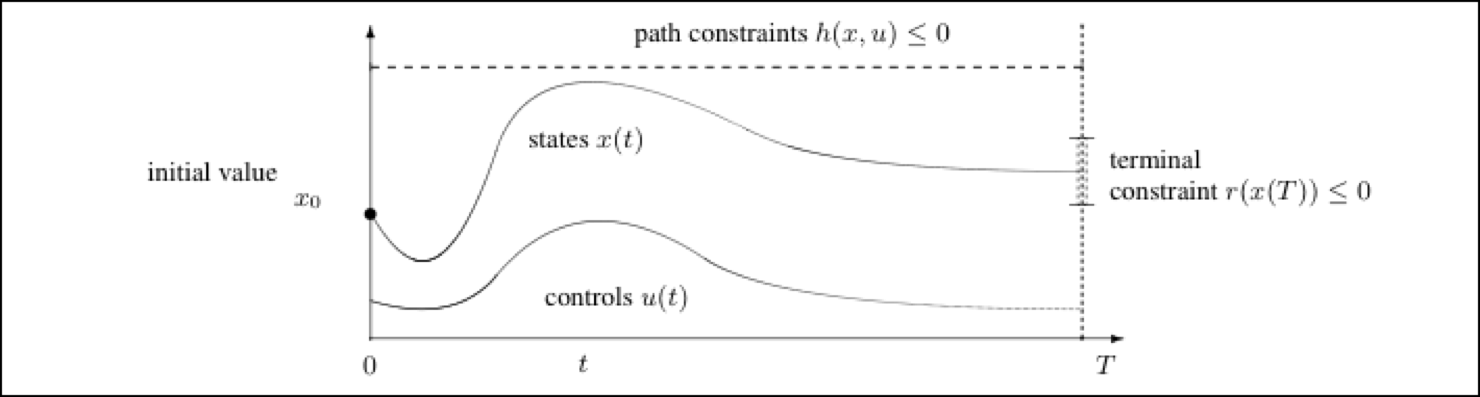
\includegraphics[width=\textwidth]{abbildungen/20160327_mpc}
\caption[Variablen und Nebenbedingungen eines optimalen Steuerungsproblems]{Variablen und Nebenbedingungen eines optimalen Steuerungsproblems \cite[S.61]{di14}}
\label{fig:opt}
\end{figure}

Für die Lösung dieses zeitkontinuierlichen Optimierungsproblems, müssen Bedingungen für die erste und zweite Ableitung erfüllt sein. Daher ist es nötig, dass das nichtlineare Optimalsteuerungsproblem zweifach stetig differenzierbar ist und damit auch das mathematische Modell des Prozesses \cite[S.~21ff.]{di14}.
Konkret können mehrere, numerische Ansätze zur Lösung des Optimalsteuerungsproblems verfolgt werden, die sich in den Zustandsraum, die indirekten und direkten Verfahren einteilen lassen. Für reale Probleme, welche sich meist durch eine Vielzahl an Nebenbedingungen auszeichnen, eignen sich insbesondere die direkten Verfahren, die auch in der Praxis am weitesten verbreitet sind \cite[S.~63]{di14}. Die Lösung beschreibt einen hinsichtlich der gewählten Kriterien optimalen Einsatz von Steuergrößen Lösung und wird als Optimalsteuerungsplan bezeichnet.
Da die Modellprädiktive Regelung nur den Rahmen dieser Arbeit beschreibt wird nicht näher darauf eingegangen und für eine theoretische fundierte Einführung in die gesamte Thematik und die einzelnen Lösungsmethoden von Optimalsteuerungsproblemen auf \cite{di14} verwiesen.

Da Modelle in der Realität den tatsächlichen Prozess nicht vollends beschreiben, wird sich der reale Prozess durch die Umsetzung des berechneten Optimalsteuerungsplans mit höchster Wahrscheinlichkeit auch nicht wie gewünscht/berechnet/vorhergesagt verhalten. Dies wird als Model-Plant-mismatch bezeichnet. Um diesen Fehler auszugleichen wurde Modellprädiktive Regelung aus der Optimalsteuerung weiterentwickelt.
Dadurch wird das Verhalten eines Prozesses in eine immer gleichweit in die zukünftige Periode hineinreichende Periode -- zu beschreiben. Hierzu bedient \acrlong{mpc} sich der Kenntnis des aktuellen Zustandes und eines physikalischen-mathematischen Modells des Systems, um dessen zukünftiges Verhalten \Gun vorherzusagen \Gob bzw. abzubilden. Des Weiteren wird versucht das Verhalten des Systems mit minimalem Aufwand zu beeinflussen, um einem eigens- oder vordefinierten Zielkriterium zu folgen \acrlong{bzw} diesem zu entsprechen.
\cite[S.~71]{di14}

Modell und MPC
Modelle reales Verhalten beschreiben,  komplexität nicht zu hoch sein um Rechenzeit gering zu  Steuerung im laufenden Betrieb zu ermöglichen.
Steuerung der Raumtemperaturregelung MPC mit Steuerungsproblem im laufenden Betrieb, jedoch nicht online, nur quasi. Immer auf Basis der aktuellen Messungen des Systemzustandes, nächster Schritt vorhersage Werte Controls. Durch dauernde Lösung können Modellfehler und Störungen ausgeglichen werden

Hohe Modellgüte bei gleichzeitig geringer Komplexität und Steigkeit


Geringe Komplexität aus Anwendung/arebitsweise mit MPC, da wiederholte Lösung nötig des Opt Problems
Stetig differenzierbar notwendig aus gradientenbasierter optimierung
Um MPC durchzuführen ist es tribiel dass modell entsprechende Güte besitzt und auch die -steuergrößen einen Einfluss.
Da Gegenläufig muss ein Kompromiss gefunden werden.


\section{Technische Grundlagen zur Kommunikation mit Bussystemen}
\label{sec:grundlagenbus}
In diesem Kapitel werden die Grundlagen von Hard- und Software beleuchtet die für die Kommunikation der Steuerung mit den einzelnen Anlagenteilen benötigt werden.
Diese umfassen zunächst Bussysteme im Allgemeinen, dann das OSI Modell für techn. Kommunikation und werden anhand des spezifischen/konkreten Anwendungsfalls Modbus erläutert.

Die Einführung wird an der Struktur von \cite{schn06} anlehnen.

\subsection{Bussysteme} 
Um allgemein Prozesse zu überwachen, zu steuern oder regeln zu können, müssen zwischen den verschiedenen Prozessbeteiligten/einheiten Informationen ausgetauscht werden. Im Kontext dieser Arbeit gilt es einen Prozess zur Temperatursteuerung/Halten zu regeln. Die Prozessbeteiligten sind hierbei technische Bauteile, Aktoren und Sensoren sowie ein Steuerungsrechner/Controller, die zusammen ein technisches System bilden, dass im Folgenden als Anlage bezeichnet wird. Die Anlage zeichnet sich dadurch aus, dass sie eine eigenständige funktionale Einheit bildet einen eigenen Zweck verfolgt, die Raumtemperaturregelung und einen Mehrwert gegenüber ihrer Einzelteile hat, was dem Zusammenspiel der einzelnen Bauteile und Geräte entspricht. 
Um den Mehrwert zu realisieren und den Zweck zu erfüllen, werden Kommunikationssysteme benötigt. Mit Hilfe derer kann Kommunikation erfolgen und die Anlage ihren Zweck erreichen.
Diese Kommunikationssysteme werden von technischer Seite oftmals als Bussysteme realisiert/umgesetzt.
Bussysteme lassen sich anhand ihrer verschiedenen Ausprägungen von Merkmalen klassifizieren. Im folgenden Abschnitt werden zunächst die Merkmale von Bussystemen zum allgemeinen Verständnis dargestellt bevor auf die konkreten Ausprägungen des später eingesetzten Modbus-Bussystems eingegangen wird.

\subsubsection{Informationsaustausch}

Die Informationen über einen Prozess und dessen Zustand, werden auf höherer Ebene durch Daten und auf unterster Ebene durch einzelne Bits repräsentiert. Der Austausch dieser Daten zwischen den einzelnen Geräten findet in Form von Telegrammen statt. Ein Telegramm besteht grundsätzlich aus den zu übertragenden Daten und zusätzlich aus Informationen zur Übertragung. Die Daten werden vor der Übertragung in Rahmen, sogenannte data frames, eingeteilt, deren genauer Aufbau abhängig vom verwendeten Kommunikationsprotokoll innerhalb des Netzwerks ist \cite[S.~11f.]{schn06}. Der Aufbau eines Telegramms am Beispiel des Modbus-Kommunikationsprotokolls wird in Abschnitt \ref{sub:modbus} erläutert und ist in \ref{fig:modbusframe} graphisch dargestellt.

\subsubsection{Netzwerk und Topologie}

Werden einzelne Prozesseinheiten miteinander über sogenannte Verbindungsleitungen, die zur Übertragung Informationen genutzt werden können, verknüpft, entstehen dabei Netzwerke und die Prozesseinheiten werden als Teilnehmer des Netzwerks bezeichnet. Ein Netzwerk lässt sich in einzelne Segmente einteilen und kann je nach Ausführung der Verbindungsleitungen und Anzahl der Teilnehmer unterschiedlich ausgeprägt sein. Anhand der geometrischen Anordnung lassen sich die folgenden, verschiedenen Netzwerktopologien unterscheiden.


Die einfachste Art, um eine Verbindung zwischen zwei Teilnehmern eines Netzwerks herzustellen, ist die sogenannte Zweipunktverbindung. Dazu sind die Netzwerkteilnehmer durch eine direkte Leitung miteinander verbunden. Jedoch steigt mit der Anzahl von Teilnehmern auch der Verbindungsaufwand überproportional an, um bei solchen vermaschten Netzwerk alle Teilnehmer miteinander zu verbinden. Dies hat für große, vermaschte Netze zur Folge, dass eine unübersichtliche große Anzahl von Schnittstellen, ein extrem hoher Verkabelungsaufwand und damit verbundene hohe Kosten entstehen. Um diese Kosten zu vermeiden, ergeben sich noch verschiedene andere Möglichkeiten zur Anordnung von Teilnehmern in Netzwerken \cite[S.~1f.]{schn06}.


Um dem hohen Verkabelungsaufwand zu vermeiden, wird bei großen Netzwerken zu einer Linienstruktur übergegangen, die auch als Bus-Struktur bezeichnet wird und in \ref{fig:bus_struktur} visualisiert ist. Charakteristisch für die Bus-Struktur ist, dass alle Teilnehmer entlang einer langen Verbindungsleitung, dem sogenannten Buskabel, angeordnet sind. Sie sind mit Hilfe von kurzen Stichleitungen an das gemeinsame Buskabel angebunden, über das die gesamte Kommunikation im Netzwerk erfolgt.
Durch diese Anordnung wird der Verkabelungsaufwand sowie die Anzahl an Schnittstellen, insbesondere für sehr große Netzwerke, stark reduziert. Jedoch wird durch Nutzung einer gemeinsamen Kommunikationsleitung die gleichzeitige Kommunikation von Teilnehmern erschwert und es müssen sogenannte Buszugriffsverfahren definiert werden, welche lediglich Regeln für Zugriff auf den Bus festlegen. Weiterhin müssen durch die Parallelschaltung alle Teilnehmer ständig alle Sendungen mitverfolgen, wodurch der Sender stark belastet wird. Die Busleitungslängen sind meist sehr lange\footnote{Diese reichen von mehreren hundert Metern bis teilweise in den Kilometerbereich, je nach Art und Einsatzort der Anwendung.}  und da die Länge auf die zu übertragende Wellenlänge bezogen nicht mehr vernachlässigbar klein ist, müssen Reflexionen durch Leitungsabschlusswiderstände an den beiden Enden der Busleitung unterbunden werden. Außerdem werden die Leitungslängen und die Teilnehmer je Netzwerksegment begrenzt\ref[S.~3f.]{schn06}.

\begin{figure}
\centering
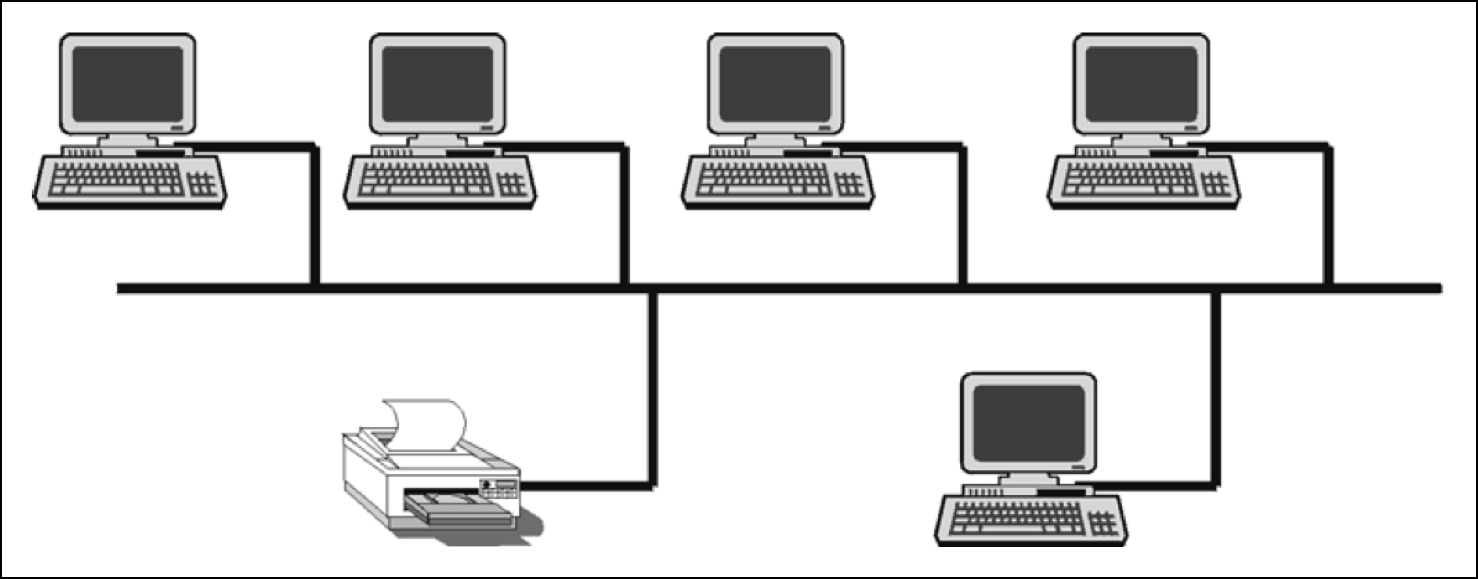
\includegraphics[width=\textwidth]{abbildungen/20160109_busstruktur}
\caption[Bus-Struktur]{Bus-Struktur aus \cite[S.~3]{schn06}}
\label{fig:bus_struktur}
\end{figure}

Ein weiterer begrenzender Faktor für die Leitungslänge ist der Fakt, dass die maximale Übertragungslänge und die maximale Übertragungsrate miteinander verknüpft sind und sich gegenseitig beschränken.
Der Leitungs- und Kapazitätswiderstand einer Leitung hängen von der Länge der Leitung ab und lassen sich durch das Ersatzschaltbild eines RC-Gliedes repräsentieren, wie in Abbildung \ref{fig:bus_impuls} a) zu sehen ist. Durch die beiden Widerstände entsteht auf der Leitung eine Impulsverzerrung \gls{timp}, die somit mittelbar von der Leitungslänge abhängt.
Je länger die Leitung wird, desto größer werden auch beiden Widerstände. Durch die erhöhte Leitungskapazität $C_{Leitung}$ erhöht sich die Ladezeit und gleichzeitig sinkt durch den erhöhten Leitungswiderstand $R_{Leitung}$ die Lastspannung $U_{G}$. Damit vergrößert sich die Impulsverzerrung \gls{timp}, wie in \ref{fig:bus_impuls} b) und \ref{fig:bus_impuls} c) dargestellt.
Dadurch wird die maximale Frequenz \gls{fmax} der Datenübertragung auf den Kehrwert der Impulsverzerrung $f_{max}=\frac{1}{\Delta t_{Imp}}$ beschränkt, da ansonsten der Empfänger den Wechsel des logischen Zustandes nicht mehr registrieren kann. In der Praxis bedeutet dies, dass die maximale Übertragungslänge und die maximale Übertragungsrate miteinander verknüpft sind und sich gegenseitig beschränken \cite[S.~4f.]{schn06}.

\begin{figure}
\centering
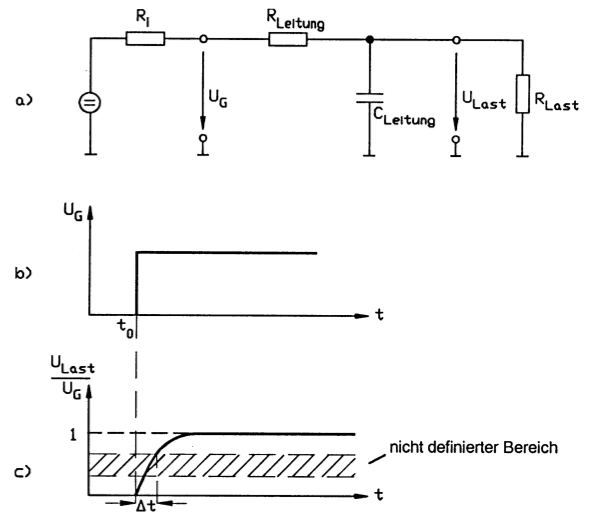
\includegraphics[width=\textwidth]{abbildungen/20160110_impulsbus}
\caption[Impulsverzerrung auf einer Leitung]{Impulsverzerrung auf einer Leitung: a) Ersatzschaltbild der Anordnung b) Ausgangsspannung des Generators c) Empfängerspannung aus \cite[S.~4]{schn06}}
\label{fig:bus_impuls}
\end{figure}

Um die Begrenzung der Leitungslängen zu korrigieren, wurde die Bus-Struktur zu einer Baumstruktur weiterentwickelt, welche in \ref{fig:baum_struktur} dargestellt ist. Darin werden einzelne Netzwerk-Segemente, also einzelne Bus-Strukturen, durch Verstärkerelemente, sogenannte  Repeater, zu einem großen Netzwerk verknüpft. Um damit jedoch größere Flächen als mit der Bus-Struktur zu vernetzen und gleichzeitig die maximale Leitungslänge und die maximale Anzahl der Busteilnehmer zu vergrößern, wird jedoch eine galvanische Trennung der Teilnehmer voneinander benötigt \cite[S.5~f.]{schn06}. Die Besonderheit in dieser Struktur liegt also darin, dass sich durch Ihren Aufbau bestehende Bus-Strukturen auch nachträglich einfach erweitern oder miteinander verknüpfen lassen. Die Bauteile zur Erweiterung von Netzwerken werden im Abschnitt \ref{sub:schnitt} Schnittstellen vorgestellt.

\begin{figure}
\centering
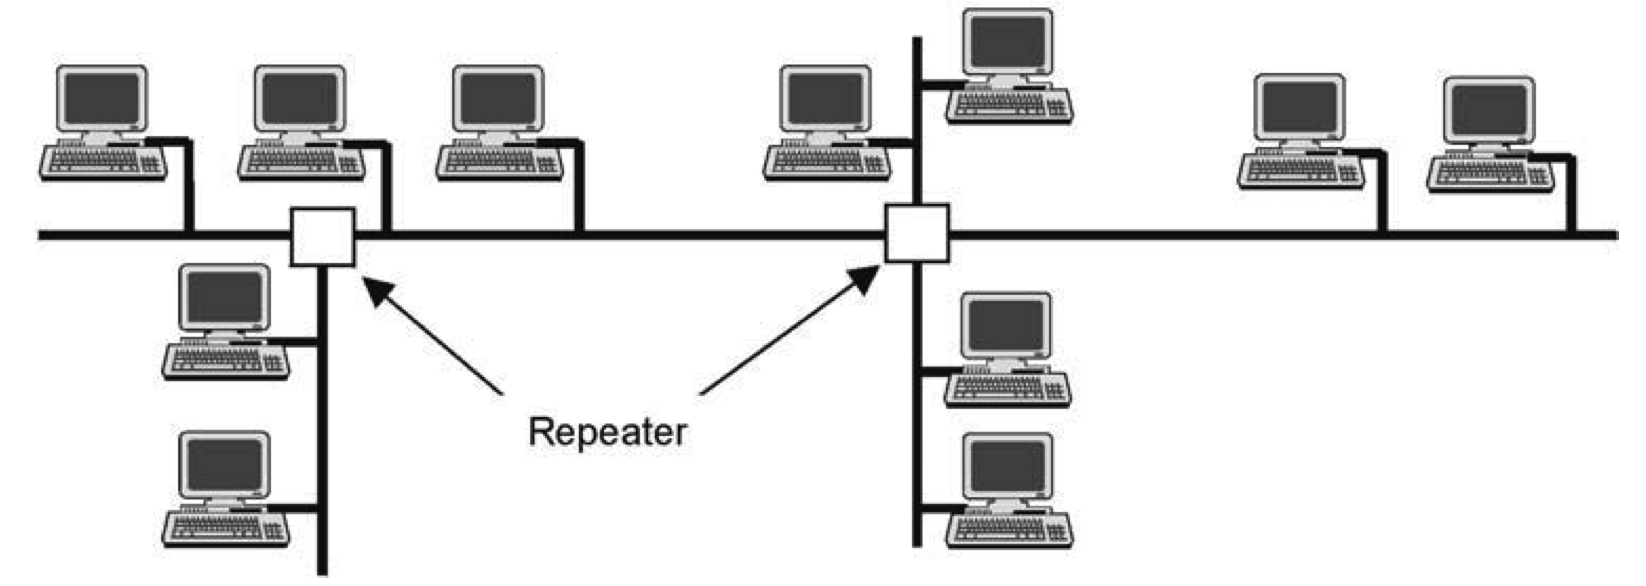
\includegraphics[width=\textwidth]{abbildungen/20160110_baumstruktur}
\caption[Baumstruktur]{Baumstruktur aus \cite[S.~5]{schn06}}
\label{fig:baum_struktur}
\end{figure}

Weitere wichtige Netzwerk Topologien, die für das Verständnis dieser Arbeit keine weitere Relevanz haben, sind die Ring- und die Stern-Struktur.
Die Ring-Struktur ist durch einen physikalischer Ring von Zweipunktverbindungen aufgebaut und gekennzeichnet durch die Kommunikation der Teilnehmer übereinander hinweg. Die Stern-Topologie hingegen ist um eine Zentralstation herum ausgebaut, die mit allen Teilnehmer verbunden ist und über die die gesamte Kommunikation abläuft. Der interessierte Leser findet in \cite[S.~6f.]{schn06} detailliertere Ausführungen.

\subsubsection{Buszugriffsverfahren}
Die meisten Netzwerktopologien kommunizieren gemeinsam über eine Verbindungsleitung. Daher werden Regeln für den Zugriff definiert, um eine reibungslose Kommunikation zu ermöglichen. Die Buszugriffsverfahren lassen sich in zwei Gruppen aufteilen, der kontrollierten und zufälligen Verfahren \cite[S.~19]{schn06}.

Bei den kontrollierten Verfahren ist der Sender bereits vor Sendebeginn eindeutig bestimmt und eine Zuteilung des Busses ist nicht notwendig. Der Buszugriff findet entweder zentral innerhalb einer Zentralstation statt, bei sogenannten Master/Slave-Verfahren, oder wird dezentral durch Steuereinheiten vorgenommen, wie z.B. beim Tokenring und Tokenbus. Ein solches Verfahren heißt echtzeitfähig, wenn die Zykluszeit zur Datenübertragung berechenbar ist, aufgrund einer Beschränkung der Länge des Übertragungsintervalls und der maximalen Datenlänge.
Bei zufälligen Buszugriffsverfahren greifen die Teilnehmer bei Bedarf auf die Verbindungsleitung zu und müssen sicherstellen, dass diese nicht gerade von einem anderen Teilnehmer belegt ist. Da nicht vorhergesehen werden kann, an welchem Zeitpunkt Informationen übertragen werden kann keine Echtzeitfähigkeit erreicht werden \cite[S.~19]{schn06}.

Das Master/Slave-Verfahren besteht in der Regel aus einer Bussteuerungseinheit, dem sogenannten Master, und mehreren passiven Teilnehmern, den Slaves. Die Kommunikation wird ausschließlich vom Master initiiert, der die Verbindung zu den Slaves aktiv durch ein Request herstellt, in welchem die angeforderten Daten sepzifiziert sind. Die Slaves treten nur nach Anfragen in Aktion und antworten darauf unmittelbar mit einer Response, die die angeforderten Daten des Masters enthält. In der Regel erfolgt die Kommunikation zyklisch zu allen Slaves gleichzeitig (Polling), damit der Master ein umfassendes und aktuelles Bild über den Systemzustand bekommt. Dadurch ergeben sich einfache Slaves, die günstig in den Bus eingebunden werden können, weil die gesamte \Gun Intelligenz\Gob im Master implementiert ist. Jedoch gilt es bei diesem Verfahren zu beachten, dass der Informationsaustausch zwischen verschiedenen Slaves längere Zeit in Anspruch nehmen kann und bei einem Ausfall des Masters das gesamte Bussystem stillliegt \cite[S.~19ff.]{schn06}.
Auf eine weitere Beschreibung der übrigen Verfahren wird aufgrund der fehlenden Relevanz für diese Arbeit verzichtet, der interessierte Leser findet jedoch bei \cite{schn06} im Kapitel Buszugriffsverfahren ausführliche Informationen.

\subsubsection{Datensicherung}

Bei der Übertragung von Informationen besteht die Gefahr von Störungen, welche sich als Fehler in einer Nachricht durch Invertierung von Bits  äußern. Störungen sind in der Regel technischer Art, wie zum Beispiel elektromagnetische Störsignale, Rauschen oder Potentialdifferenzen, und gegen einen Großteil lassen verschiedene Vorkehrungen treffen. Dadurch ergibt sich die Möglichkeit Störungen vorzubeugen oder diese nach Einsatz zu beseitigen. Der erste Ansatz ist also eine Verminderung des Auftretens durch technische Vorkehrungen, wie zum Beispiel Schirmung der Kabel, galvanische Trennung von Netzwerken oder differenzielle Signalübertragung. Der zweite Ansatz beschäftigt sich mit der Überwachung des Nachrichtenverkehrs und dem Ausbessern/Gegenmaßnahmen bei Fehlern \cite[S.~30]{schn06}.

Auf dem Gebiet der Buskommunikation entspricht wird eine Information oder Nachricht oder Telegramm codiert. Es werden stets Transparente Codes betrachtet, Welche bitorientiert sind. Dabei sind jegliche Kombination von Bits erlaubt und man kann allein Aus der Folge der Blitz nicht auf einen Fehler schließen.
Definition Telegramm und Bit(0 und 1)

Die Vorkehrungen technischer Art Können Sind in aller Regel in den Spezifikationen der einzelnen Bussysteme enthalten, daher Werden diese nicht weiter beschrieben und lediglich die Überwachung und Ausbesserung das Nachrichtenverkehrs erläutert.
Bei der Übermittlung von Nachrichten können drei Arten von Fehlern auftreten:
Der Fehler kam erkennbar und korrigierbar sein,
Erkennbar und nicht korrigierbar
Oder nicht erkennbar und damit auch nicht korrigierbar.

Kann der Fehler erkannt werden ist bereits ein großer Teil der Arbeit getan. 

Fehlermaße sind
die Bitfehlerrate p = Anzahl fehlerhafter bits/ gesamtzahl gesendete bits, schlechtester Wert ist p=0,5, da durch invertierung immer wieder umstellbar. üblich in Technik $p=10^{-4}$.
ARQ(Error detection and automatic request repeat) ist normale Reaktion auf erkannte Fehler, dass eine einfache Wiederholung der Übertragung.

Restfehlerrate R ist eine wichtige Kennzahl weil, sie die unerkannten, fehlerhaften Bitfolgen die nach der Anwendung von Fehlererkennungstrategien noch verbleiben misst. R = Anzahl unerkannt fehlerhafter Bitmkombinationen/Gesamtlänge in Bits der Information.
-->Maß für Unversehrtheit der Daten

Telegrammeffizienz auch wichtig, weil sie eine Aussage erlaubt wie viel Infomrtionen tarnsportiert werden können und sie steht im Gegensatz zur Restfehlerquote, je sicherer Übertragung desto weniger Effizienz. E = fehlerfreie Infobits/Gesamtzahl übertragene bits(incl. Adresse Erro check usw.)
\cite[S.~31ff.]{schn06}

Die genauen Berechnungen der Wahrscheinlichkeiten und der mittleren Zeit zwischen zwei Fehlern sind und noch viel mehr Details finden sich im Kapitel Datensicherung in \cite[S.~31f.]{schn06} zu finden.

Um Fehler systematisch zu erkennen, existieren verschiedene Fehlererkennungsstrategien. Die einfachste ist der Paritätsbit, der lediglich die Quersumme des Telegramms angibt, P=0 für eine ungerade und p=1 für eine gerade Quersumme. Damit können diejenigen Fehler entdeckt werden, die eine ungerade Anzahl an Bitflips haben, die mit geraden leider nicht. Eine Erweiterung der Paritätssicherung ist die Blocksicherung, bei der die Paritäten über ein Array aus mehreren Telegrammen überprüft werden kann \cite[S.~34f.]{schn06}.

\begin{figure}
\centering
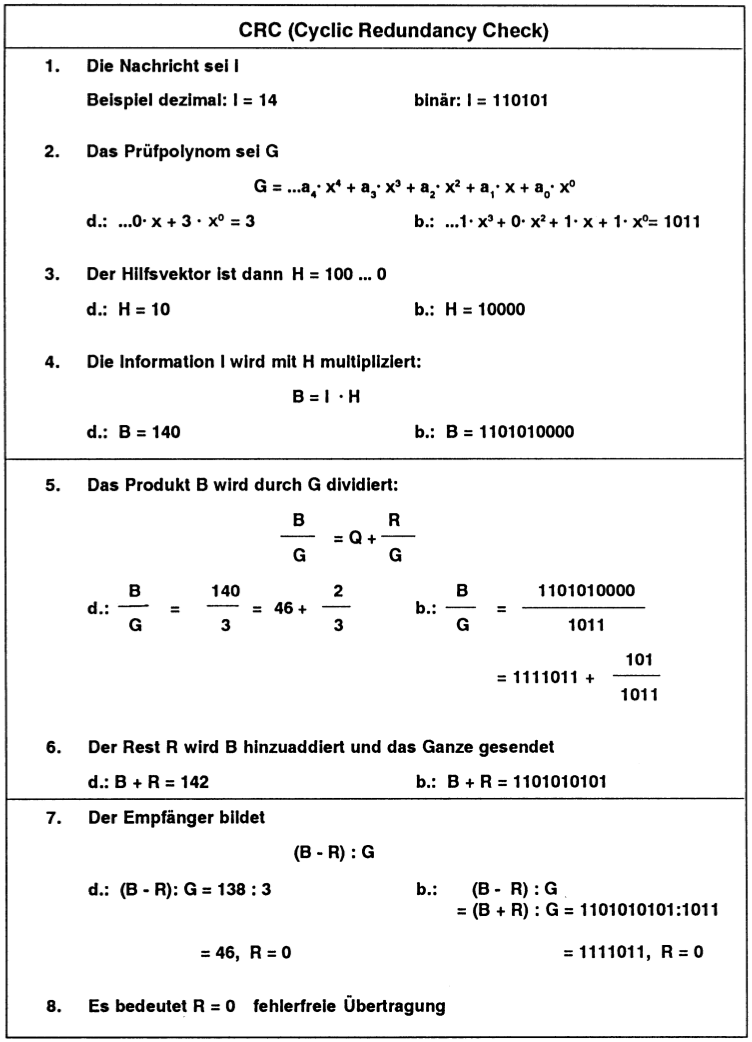
\includegraphics[width=\textwidth]{abbildungen/20160314_crc}
\caption[\textit{Cyclic Redundancy Check}]{\textit{Cyclic Redundancy Check} aus \cite[S.~38]{schn06}}
\label{fig:crc}
\end{figure}

Beim sogenannten Cyclic Redundancy Check, in der Literatur häufig als CRC-Check bezeichnet, wird ein Telegramm als Zahl aufgefasst. Im Sender wird diese Zahl durch das Generatorpolynom G geteilt. Das Ergebnis wird verworfen, lediglich der Rest bei der Division wird an das Telegramm angehängt. Der Empfänger dividiert das empfangene Telegramm durch dasselbe Polynom G und falls sich ein Rest von 0 ergibt, war die Übertragung fehlerfrei. Dadurch lassen sich abhängig vom Generatorpolynom G unterschiedliche Güten der Fehlererkennung realisieren. In \ref{fig:crc} sind die Vorgänge beim Cyclic Redundancy Check graphisch zusammengefasst.



\subsubsection{Schnittstellen}
\label{sub:schnitt}

Die physikalische Übertragung der Daten/Telegramme kann über verschiedenste Schnittstellen geschehen und erfplgt binär. Je nach Topologie des Bussystems und Protokoll, kann die Datenübertragung seriell oder parallel geschehen wie in \ref{fig:seriell} zu sehen. Bei einer parallelen Datenübertragung werden immer mehrere Bits gleichzeitig übertragen, weshalb eine hohe Übertragungsgeschwindigkeit erreicht werden kann, jedoch eine aufwändige im Sinne eines vermaschten Netzes notwendig ist. Daher erfolgt in der Praxis eher eine serielle Datenübertragung, also die einzelne Übertragung von bits nacheinander über eine Leitung, wie sie zum Beispiel mit einer Bus-Struktur möglich ist \cite[S.~13]{sch08}.


\begin{figure}
\centering
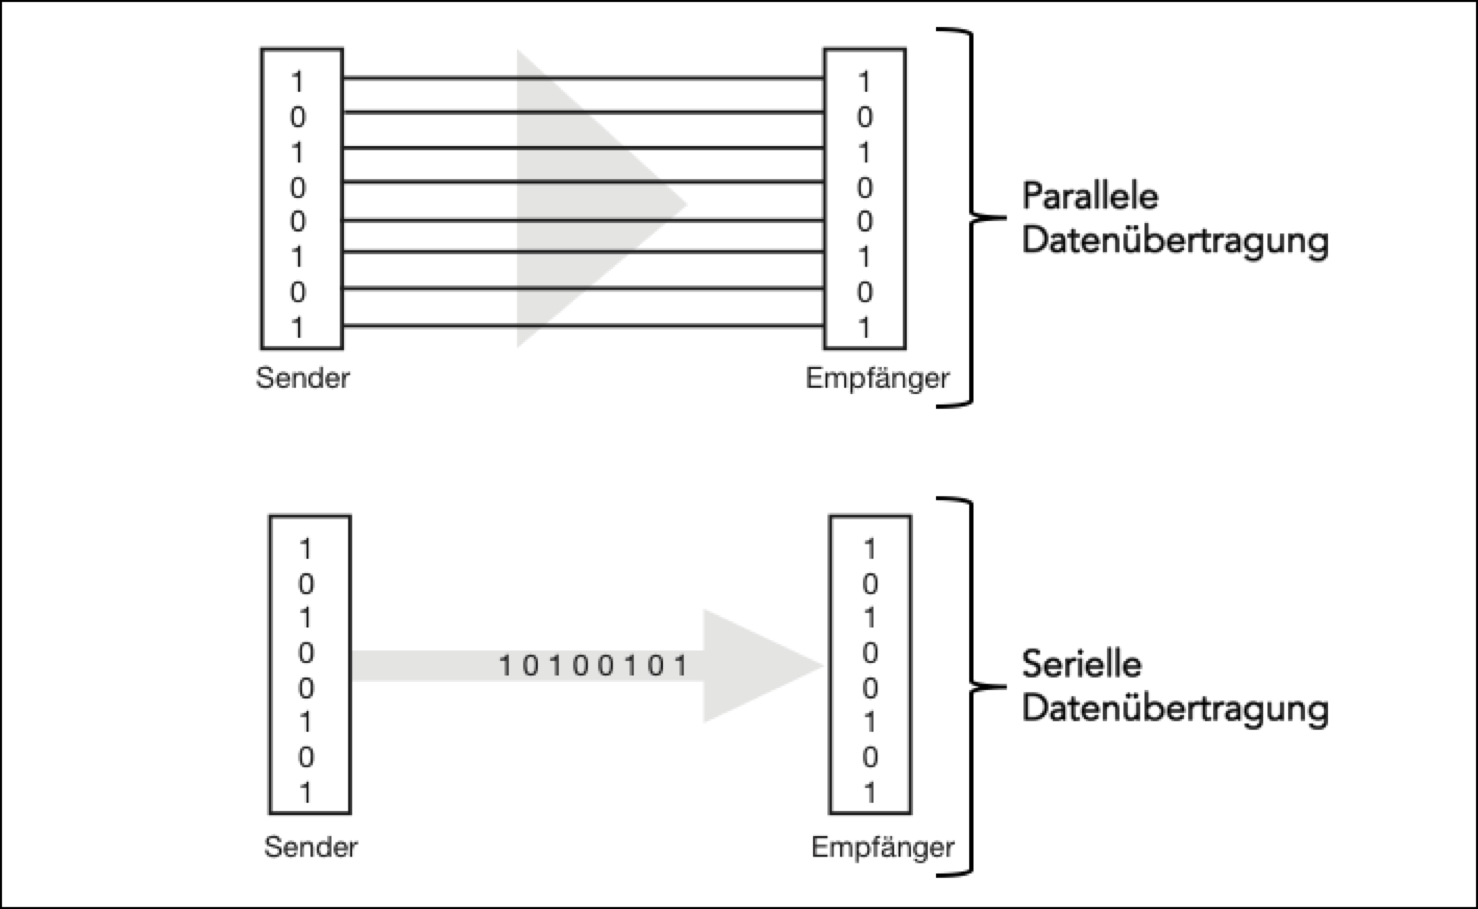
\includegraphics[width=\textwidth]{abbildungen/20160314_seriell}
\caption[Parallele und serielle Datenübertragung]{Parallele und serielle Datenübertragung aus \cite[S.~13]{sch08}}
\label{fig:seriell}
\end{figure}


Bei der binären Datenübertragung werden lediglich zwei Zustände unterschieden, deren Signalwerte einen High-Pegel \gls{phigh} und einen Low-Pegel \gls{plow} besitzen, die durch einen Bereich, in dem das Signal nicht definiert ist, voneinander getrennt sind \cite[S.~9]{sch08}.
Die Geschwindigkeit der Datenübertragung wird in der Einheit Baud gemessen und definiert als übertragene Bits pro Sekunde (Bps)\cite[S.~22]{sch08}.

Die gängigsten Übertragungsverfahren sind elektrische und optische Schnittstellen. Die elektrischen Schnittstellen gliedern sich wiederum in Strom- und Spannungs-Schnittstellen auf. Im weiteren Verlauf der Arbeit sind lediglich die Spannungsschnittstellen EIA\footnote{Abkürzung der Normen und Standards die von der Electronic Industries Alliance entwickelt wurden.} 232 und EIA 485, welche auch als EIA 232 und EIA 485 beziechnet werden, relevant, weshalb der interessierte Leser weitere Informationen zu weiteren Schnittstellen in \cite[S.~13ff.]{sch08} und \cite[S.~57ff.]{schn06} findet.

Die EIA 232 Schnittstelle ist wie bereits erwähnt eine Spannungsschnittstelle, die für Punkt-zu-Punkt Verbindungen geeignet ist und deren Pegel in \ref{fig:rs232} zu sehen sind. Die Pegel sind für Spannungen zwischen $-3V<p_{high}<-15V$ als logische \Gun 1\Gob, der Low-Pegel für Spannungen zwischen $-3V<p_{low}<-15V$ als die logische \Gun 0\Gob definiert. Im Intervall $[-3V,3V]$ ist das Signal nicht definiert, weshalb dieser Bereich möglichst schnell durchlaufen werden sollte. Da der Signalpegel von der Datenleitung hin zur Masse gemessen wird kann er nicht symmetrisch sein und ist damit erdunsymmetrisch. \cite[S.~57f.]{schn06}

\begin{figure}
\centering
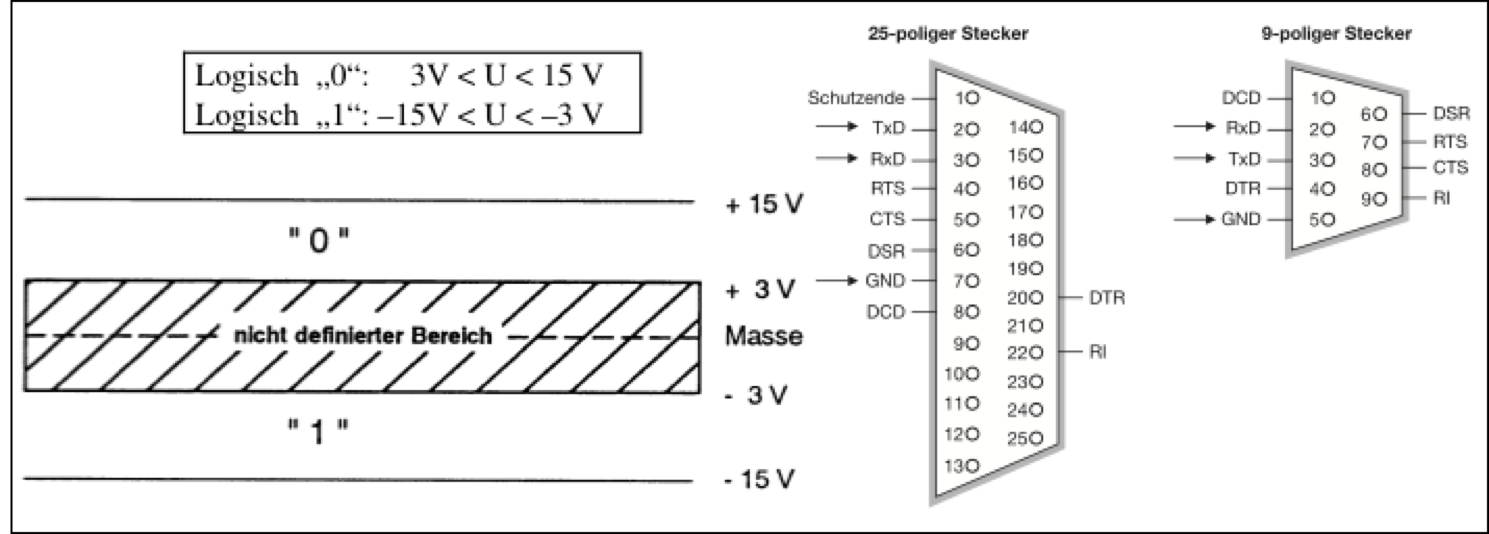
\includegraphics[width=\textwidth]{abbildungen/20160314_rs232}
\caption[Spannungspegel und Stecker der EIA 232-Schnittstelle]{Links: Spannungspegel EIA 232-Schnittstelle aus \cite[S.~57]{schn06} \newline Rechts: Stecker EIA 232-Schnittstelle aus \cite[S.~14]{sch08}}
\label{fig:rs232}
\end{figure}

Typischerweise steht eine solche Schnittstelle jedem Rechner als COM-Port zur Verfügung und in der Automatisierungstechnik werden nur die RxD (Receive Data), TxD (Transmit Data) und GND Leitungen, die ein gemeinsames Bezugspotenzial definiert, verwendet. Wichtig bei der Verkabelung ist, dass die übertragende Leitung TxD immer mit der empfangenden Leitung RxD verbunden ist \cite[S.~14f.]{sch08}.

%Here we go
Die EIA 485 Schnittstelle ist ebenfalls eine Spannungsschnittstelle, die jedoch für Mehrpunktverbindungen geeignet ist und die in der Norm ISO
8482 beschrieben ist. Die Signalübertragung erfolgt über zwei Übertragungsleitungen, die in der Regel als verdrilltes und abgeschirmtes Zweidrahtleitung ausgeführt sind. Die Signalpegel entsprechen der Differenzialspannung $U_{AB}$ zwischen den beiden Leitungen, die innerhalb des Intervalls von $[-7V,12V]$ bezogen auf die Masse liegen muss. Durch das verdrillte Leitungspaar, wirken sich mögliche Störgrößen auf die Spannung beider Leitungen gleichermaßen aus, wodurch die Spannungsdifferenz unverändert bleibt und eine erhöhte Störfestigkeit gegenüber der EIA 232-Schnittstelle erreicht wird.
Bei der Pegelfestlegung werden für Empfänger und Sender gibt es verschiedene Vorgaben, wie in \ref{fig:rs485} graphisch dargestellt. So müssen die Sender eine Differenzspannung zwischen $-1,5V<U_{AB}<-5V$ für logische \Gun 1\Gob und $1,5V<U_{AB}<-5V$ für logische \Gun 0\Gob leisten können. Empfänger hingegen müssen in der Lage sein Spannungsdifferenzen von $U_{AB}<-0,3V$ als logische \Gun 1\Gob und $0,3<VU_{AB}$ als logische \Gun 0\Gob zu detektieren und zu interpretieren \cite[S.~59ff.]{schn06}.

\begin{figure}
\centering
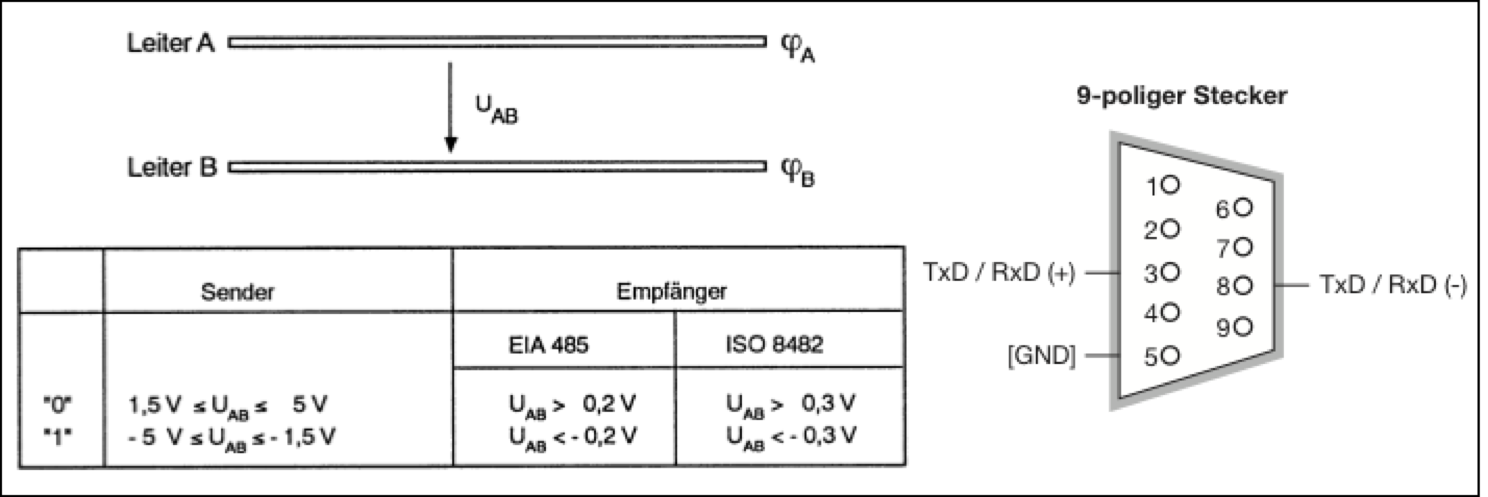
\includegraphics[width=\textwidth]{abbildungen/20160314_rs485}
\caption[Spannungspegel und Stecker der EIA 485-Schnittstelle]{Links: Spannungspegel EIA 485-Schnittstelle aus \cite[S.~60]{schn06} \newline Rechts: Stecker EIA 485-Schnittstelle aus \cite[S.~19]{sch08}}
\label{fig:rs485}
\end{figure}

Es besteht ein geringer Installationsaufwand und die Datenübertragung erfolgt über die TxD/RxD + und TxD/RxD - Leitungen, ein gemeinsames Bezugspotential über die GND Leitung wird nicht zwingend benötigt, jedoch wird ein Leitungsabschluss an beiden Enden des Buskabels benötigt.  \cite[S.~19f.]{sch08}.


Um Netzwerk zu erweitern, können verschiedene Bauteile eingesetzt werden. Sogenannte Repeater sind aktive Bauteile, die lediglich einen kurze Zeitverzögerung verursachen und nur Netzwerke der selben Schnittstelle miteinander verbinden kann. Er ist ein aktives Bauteil, dass das Datensignal lediglich verstärkt, indem er die empfangenen Bits blind kopiert und verstärkt auf das angeschlossene Netzwerk überträgt, weshalb er für die Kommunikationsteilnehmer unsichtbar ist \cite[S.~79f.]{schn06}.

Eine Möglichkeit um Netzwerke verschiedener Art zu verbinden bieten Bridges und Gateways. Erstere werden auch als Schnittstellenumsetzer bezeichnet und kommen zum Einsatz, wenn trotz gleichem Übertragungsprotokoll genutzt unterschiedliche physikalische Schnittstellen oder Übertragungsmedien genutzt werden sollen \cite[S.~80f.]{schn06}. Er erkennt die Datenflussrichtung automatisch und wandelt die Pegel der Schnittstellen in den jeweils anderen um \cite[S.~21]{sch08}
Die sogenannten Gateways dienen der Kopplung von Netzwerken, die verschiedene Architekturen aufweisen, also neben unterschiedlichen physikalischen Schnittstellen auch andere Übertragungsprotokolle verwenden. Das Gateway ist demnach umfassender als die Bridge und erweitert deren Funktionen um die Übersetzung der Signale von einen Übertragungsprotokoll in das jeweils andere \cite[S.~84f.]{schn06}.



\subsection{OSI-Kommunikationsmodell}

Aufgrund der großen Anzahl verschiedener technischer Systeme existieren auch viele verschiedene Arten der Kommunikation untereinander. Bei der genaueren Betrachtung der Kommunikation wird ersichtlich, dass diese oftmals ähnlich abläuft und sich durch ein Meta-Schema beschreiben lässt \cite[S.~8]{schn06}. Um die Kommunikation auch über verschiedenen Systeme hinweg zu ermöglichen und sie zu formalisieren, wurde von der \textit{International Organization for Standardization} 1984 ein abstraktes Referenz-Modell entwickelt, dass in der \textit{ISO-Norm 7498-1} beschrieben ist. Es dient der Entwicklung und Verbesserung von Standards für den Informationsaustausch sowie als Referenz für bestehende Standard um eine gewisse Konsistenz zu wahren \cite[S.~1]{osi96}. Das Ziel bei dem Entwurf des Modells war es, eine Menge von Standards zu schaffen um autonomen Systemen die Kommunikation untereinander zu ermöglichen \cite[S.~4]{osi96}.

Das sogenannte \acrlong{osi} wird zunächst allgemein erläutert, da die Kommunikation von technischen Systemen im Rahmen der Arbeit eine zentrale Rolle spielt, und wird anschließend im Anwendungskontext mit den eingesetzten Protokollen und Schnittstellen referenziert.

Zunächst wird im Standard definiert, womit sich das Modell beschäftigt und abgegrenzt welche Aspekte im Modell keine Berücksichtigung finden \cite[S.~3]{osi96}:

\begin{quote}
\textit{\Gun OSI is concerned with the exchange of information between open systems (and not the internal functioning of each individual real open system).\Gob}
\end{quote}

Das \acrshort{osi} beschäftigt sich also zentral mit dem Austausch von Informationen zwischen verschiedenen offenen Systemen und allen dabei anfallenden Aktivitäten. Diese sind sehr umfangreich und lassen sich in folgende Bereiche gliedern \cite[S.~3f.]{osi96}:

\begin{itemize}
	\item Der Austausch von Informationen zwischen offenen Systemen,
	\item die physischen Medien zur Verbindung von offenen Systemen und deren Transportmöglichkeit von Informationen,
	\item die Vernetzung von offenen Systemen,
	\item die Interaktion zwischen offenen Systemen und deren Fähigkeit zur Kooperation bei der Datenübertragung.
\end{itemize}

Bezogen auf den Austausch von Informationen überschneiden sich die physische Verbindung und die Vernetzung und entsprechen zusammen der Infrastruktur und deren Architektur, die zur Übertragung zur Verfügung steht. Die Interaktion umfasst weitaus mehr Aufgaben: Neben der Synchronisation der Prozesse, die Daten austauschen wollen, muss auch die Darstellung der auszutauschenden Daten und eventuell notwendige Transformationen beachtet werden, um eine Kompatibilität unterschiedlicher Systeme zu erreichen. Weitere wichtige Aufgaben sind die Datenspeicherung, deren Integrität und die Sicherheit beim Austausch hinsichtlich Fehler und Einsicht von Außen \cite[S.~4]{osi96}.
Es ist leicht zu erkennen, dass die technische Kommunikation einen sehr umfangreichen und komplizierten Prozess darstellt. Daher wird der Kommunikationsprozess im \acrshort{osi} stark abstrahiert und in sieben abstrakte Ebenen gegliedert. Die einzelnen Ebenen sind in \ref{fig:osi} dargestellt und dienen dazu verschiedene Aufgaben des Kommunikationsprozesses in Teilaufgaben zusammenzufassen.

\begin{figure}
\centering
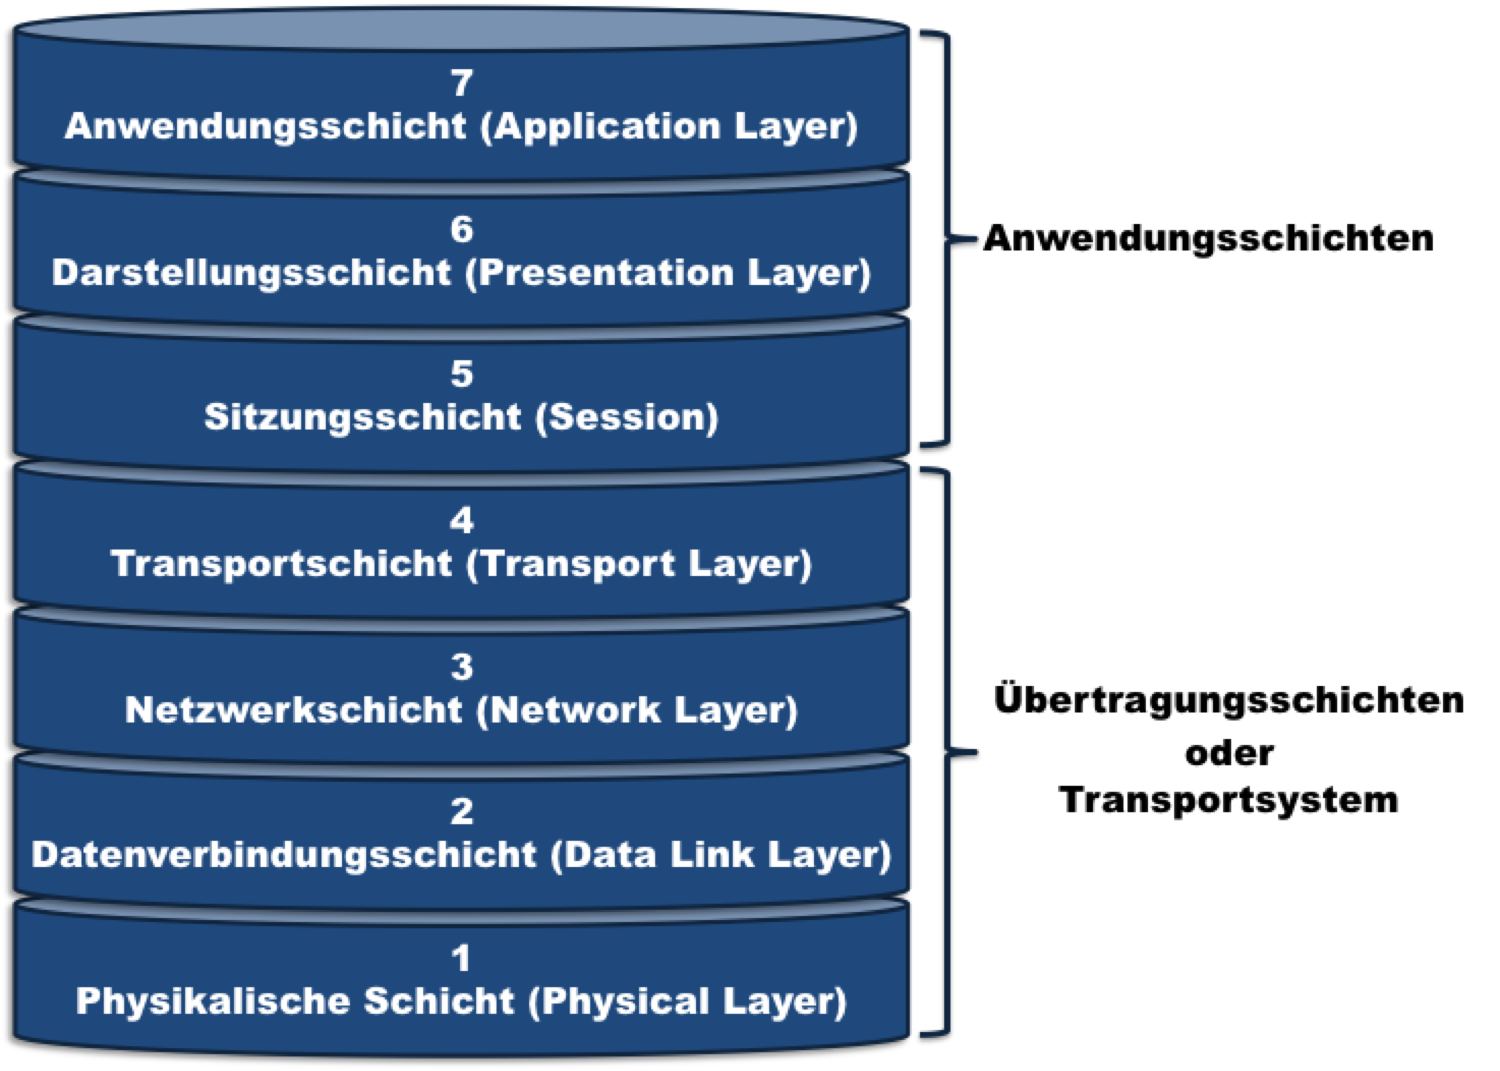
\includegraphics[width=\textwidth]{abbildungen/20160112_osi}
\caption[Die sieben Schichten des Open System Interconnection Modells]{Die sieben Schichten des \textit{Open System Interconnection} Modells verändert nach \cite[S.~10]{schn06} und \cite[S.~28]{osi96}}
\label{fig:osi}
\end{figure}

Die Ebenen werden Schichten genannt und haben klar definierte Aufgaben und Schnittstellen zu ihren Nachbarschichten. An diesen Schnittstellen werden Dienste bereitgestellt, die von den anderen Ebenen genutzt werden können. Durch diesen Aufbau können einzelne Schichten einfach bearbeitet oder ausgetauscht werden, ohne die Gesamtfunktionalität zu gefährden. Außerdem kann ein System auch aus Komponenten verschiedener Hersteller zusammengesetzt werden, womit diese Architektur nachweislich als Basis für offene Systeme dient. In \ref{fig:osi} ist ebenfalls dargestellt, dass die Schichten eins bis vier auch als Übertragungsschichten beziehungsweise Transportsystem zusammengefasst werden, weil sie für die Datenübertragung zwischen Systemen als gemeinsame Aufgabe haben. Die Schichten fünf bis sieben werden als Anwendungsschichten bezeichnet weil sie bei der Datenübertragung die Zusammenarbeit zwischen der Anwendersoftware und dem Betriebssystem sicherstellen \cite[S.~8f.]{schn06}.

Die Schnittstellen/Dienste zwischen den Schichten werden als Service Access Points bezeichnet und besitzen jeweils eine eindeutige Adresse, die oberhalb liegende Schicht ist der Service user, da er den Service daer unterhalb liegenden Schicht nutzt, dem service provider. Die Dienste können in verbindungsorientierte und verbindungsunabhängige unterschieden werden.
Für den Datenausatausch stehen folgende Dienste zur Verfügung
Bei der Abhandlung der Dienstaufgaben stehen die vier Dienstvorgänge der Client/Server Architektur zur Verfügung, die zusammengefasst in \ref{fig:vorgang} abgebildet sind \cite[S.~2f.]{mod06tcp} :

request - Anforderung
indication - Meldung
response - Antwort
confirmation - Bestätigung
Bestätigten Diensten stehen alle vier Vorgänge zur Verfügung, unbestätigten lediglich die Anforderung und Meldung.
Typische Dienste sind Connect, disconnect, data

\begin{figure}
\centering
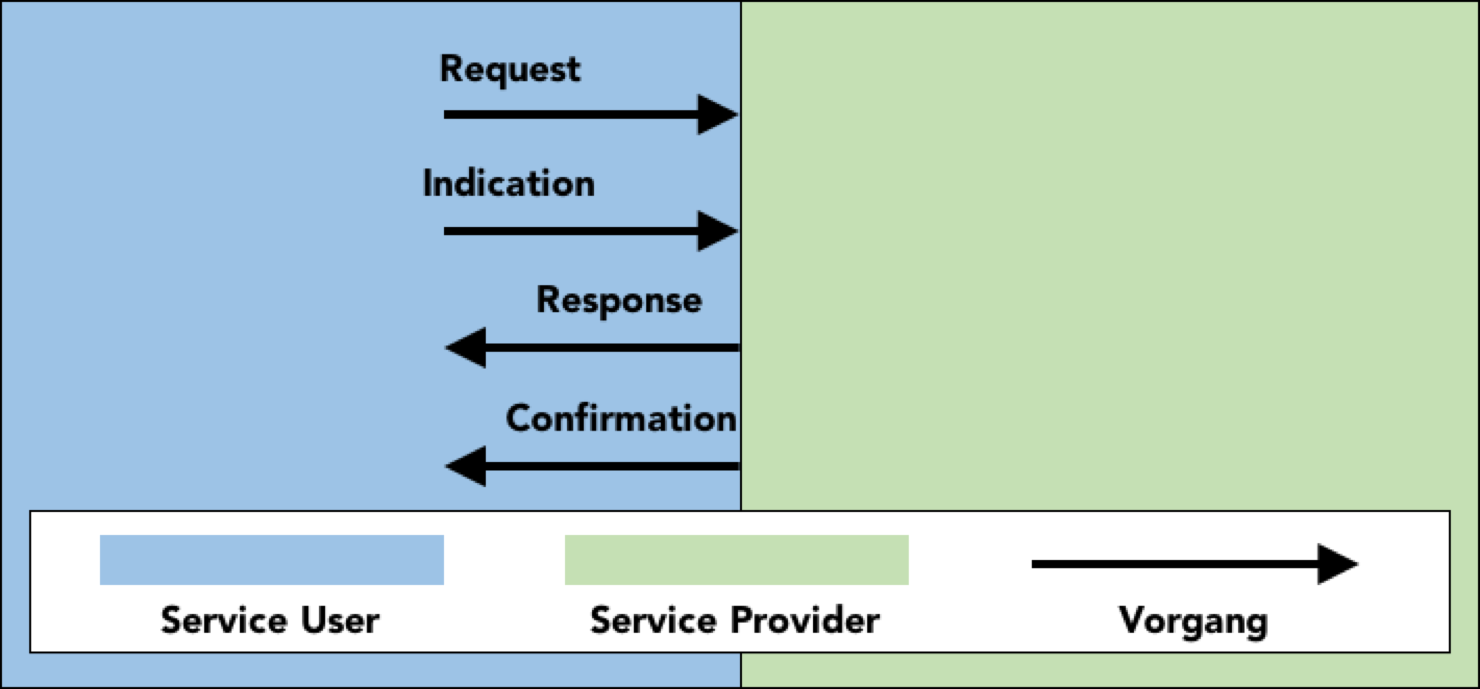
\includegraphics[width=\textwidth]{abbildungen/20160310_vorgang}
\caption{Die vier Dienstvorgänge}
\label{fig:vorgang}
\end{figure}

\cite[S.~14f.]{schn06}.

Im Folgenden wird kurz auf die einzelnen Schichten von Unten nach oben eingegangen bevor das Zusammenwirken der einzelnen Schichten anhand eines Beispiels verdeutlicht wird. %Evtl raus

Die erste, physikalische Schicht stellt die mechanischen und elektrischen Möglichkeiten zur physischen Verbindung von Systemen zur Verfügung, um die Datenübertragung der einzelnen Bits zu ermöglichen \cite[S.~49f.]{osi96}. Sie legt also die mechanischen und elektrischen Eigenschaften der Übertragung fest, also die Endsystemkopplung (Stecker), die Kabelspezifikationen und die Zuordnung der Anschlüsse sowie die Art der Codierung und die Spannungspegel zur Übertragung. In der Regel werden dazu bestehende Normen genutzt, wie zum Beispiel die elektrischen Übertragungsstrecke nach EIA 485-Norm, welche im Folgenden noch erläutert wird.

Ein wichtiger Aspekt der Schicht ist es, dass die Spezifikation der Strecke und nicht das physikalisches Medium selbst Teil der Schicht eins ist, denn die Kommunikation ist unabhängig von der konkreten Ausprägung der Schicht \cite[S.~9]{schn06}.

%Here We Go
Die zweite Schicht betrachtet Kommunikation zwischen zwei systemen. Deshalb stellt die Datenverbindungsschicht, stellt funktionale und prozedurale Möglihckeiten für den verbiindungsaufbau/trennung erhaltung und den Transfer von Dateneinheiten Verfügung. Ermögliocht dem Netzwerkschucht die Kontrolle über die Verbindung von Data circuits physikalisch, sowie fehlerabfangen der physikalsichen schicht \cite[S.~46f.]{osi96}
Aufgabe ist sicherer transport von Station zu station. Datensicherung --> Verpacken um Übertragungsfehler erkenntlich zu machen in data frames. In Frames sind die maximale Anzahl Datenbits für Rohdaten spezifiziert, weiterhin wird Information zur Übertragung hinzugefügt. Die zusatzinfo kann Prüfsumme und Anfang und Ende des Rahmens enthalten oder quittierung eines telegramms und dient dazu fehlerhafte Übertragung oder etwas verloren gegangen zu überprüfen. MAC mit Schicht eins, LLC mit Schicht drei.
Wuelle Wiki bisher
MAC regelt den Zugriff auf das ohyische Medium zur Kommunikation, kotrolliert oder konkurriert.
LLC verteilt die Daten passend in Schicht drei und gibt die Daten von schihct drei an passende MAC für schicht eins weiter und fügt Diese Infos von oben hinzu (Adressen Empfönger und Sender und zusatzinfo wie control für Steurung von Datenfluss oder so).

Wichtig Die schicht hat jedoch keine Kenntnis über Inhalte der Daten!\cite[S.~9ff.]{schn06}

% EIG bei 3 evtl schon bei 2 mit LLC in zusammenahng
verbindungsloser Dienst heisst keine Verbindung zwischen Kommunikationspartnern, Datenpakete werden wie Brief ganz in Netzwerk gespeist mit Zieladresse versehen und weitertransportiert, ohne beeinflussung des transportweges durch benutzer des netzwerkdienstes. Später ist Modbus ein Beispiel dazu erklärt.
verbindungsorientierte Dienste heisst ein virtueller Kanal zwischen kommunikationspartnern wird zur Verüfung gestellt, eingeriechtet: Verbindungsaufbau, Datenautausch, Verbindungsabbau, wie telefongespräch. \cite[S.~11f.]{schn06}


Die dritte Schicht beschäftigt sich mit dem Netzwerk als Ganzes. Die Aufgaben der Netzwerkschicht hängen ein wenig ab von verbindungsorientierung Daher beschäftigt sie sich mit dem Aufbau , der erhlatung und Datenaustasuch und dem trennen von Netzwerk Verbindungen zwischen offenen systemen i Netzwerk, also schnittstellen. weietrhin ist sie für den Transport von Daten im netzwerk zustaändig, also insbeonsdere auch für die Festelgung der Route(Wegsteuerung) der Daten im Netzwerk \cite[S.~41f.]{osi96}.
Also Kontrolle von Verkehr im Netzwerk, d.h. Anzahl Pakete im Netzwerk, Staus \cite[S.~11f.]{schn06}


Die vierte Schicht ist die Transportschicht und zuständig für die transparente Übertragung von Daten zwischen Prozessen und ist völlig unabähngig bzw losgelöst von den Gedanken an Kosten und Verlässlichkeit der Datenübertragung, da dies aufgaben der unteren schichten sind. Sie kümmert sich um die optimale nutzung von Netzwerk services/Nutzung \cite[S.~37f.]{osi96}.
Adressierung der Teilnehmer, Aufbau und Abbau für Transportverbindung wzischen Kom.Partner prozessen(Sammel Einzel Mehrere), Fehlerbehalndlung verbidnung und flusskontrolle, Synchronisierung der dtaenaustauschenden Prozesse.Zerlegung der Daten aus Sitzugnsschicht in Transportierbare Einheiten. Internetworking, Umsetzung verschiedener Protokolle Gateway Aufgaben. Aufbau Verbindung legt Art fest, Punkt zu Punkt oder Broadcast/Multicast (Alle bzw einige Teilnehmer gleichzeitig) \cite[S.~12f.]{schn06}.

Die fünfte Schicht, die Sitzungsschicht, startet eine Sitzungsverbindung mit bestimmter Adresse wenn dieser Prozess von einer höheren Schicht angefordert wird. Diese Verbindung dient dazu, den  dialog von kooperiendnen Porzesse auf der eines höhreren Darstellungsbene durch eine Sitzungsverbindung zu synchronisieren und deren Datenaustausch zu organisieren. verknüpft die Sitzungsadressen mit den Transportadressen, also die Anwendungsschiten mit dem Transportsystem \cite[S.~35]{osi96}.
Benutzung des Transportsystems über die Schnittstelle zur Transportschicht. Je nach Funktionen der höheren Schihcten entsprechender Funktionsumfang
BCS Basic Combined Subset - Verbindungssteuerung und Datenübertragung
BAS Basic Activity Subset - Aktivitätsverwaltung
BSS Basic synchronized Subset - Synchronisierung
\cite[S.~13]{schn06}.


Die sechste Schicht, die Darstellungsschicht ist nach \cite[S.~33f.]{osi96} für die Darstellung der Daten die von Anwendung-Entitäten entweder kommuniziert oder bei deren Kommunikation referenziert werden. Sie stellt außerdem eine gemeinsame Represantion der übertragenen Daten dar zwischen Anwendungs-Entitäten und befreit diese dadurch von Syntaxabhängigkeiten.
\cite[S.~13f.]{schn06} stellt fest, dass die Dienste die der Darstellung der transferierten Daten dienen wie die Codierung der zu übertragenden Daten, der verwendete Zeichensatz und die Darstellung der Daten auf dem Bildschirm oder Drucker. Semantik/Syntax beim Nachrichtenaustausch und der beiden Kommunizierenden Prozesse. Evtl Komprimierung um Zeit und Kosten zu sparen .


Die siebte und letzte Schicht stellt lediglich eine Möglichkeit für Anwendungsprzesse zur Verfügung um auf die OSI Umgebung zuzugreifen. Jeder Anwendung stellt im OSI genau einen Anwendungsprozess dar, verschiedene Anwendungsprozesse für verschiedene Anwendungen und vice versa \cite[S.~32]{osi96}
stellt Funktionen bereit, mit denen der Benutzer auf das Kommunikationssystem zugreifen kann, wobei der Benutzer idR ein Computerprogramm und kein Mensch ist. \cite[S.~14]{schn06}

Im folgenden werden die verwendeten Modbus Protokolle und Spezifikation ind Anwendung Berzug zum OSI Modell gebracht um den praktischenNutzen davon klar zu machen.


\subsection{Modbus Kommunikationstechnologie}
\label{sub:modbus}

Zunächst erfolgt die Einordnung ins OSI Modell und anschließend eine Klassifizierung der Spezifikationen gemäß der zuvor von Bussystemen.

Das Modbus Protokoll teilt sich auf verschiedene Protokolle auf, zum einen auf das Application Layer Messaging Protocol auf oberster Ebene, welches auf das Modbus Over Serial Line Protocol sowie das Ethernet TCP/IP Protokoll aufbaut.
Das Application Layer Messaging Protocol lässt sich im OSI Referenzmodell in die siebte und oberste Schicht(Anwendungsschicht) einordnen wie in \ref{fig:modbusosi} dargestellt. Bei der Nutzung des Modbus over Serial line Protocol implementiert diese die zweite Schicht und die Ebenen drei bis sechs sind leer implementiert. Als physikalische Schicht werden die Übertragungsstandards nach EIA 485 oder nach EIA 232 \cite[S.~2]{mod06ser}.
Anstatt des Over serial line kann auch das Modbus Messaging On TCP/IP Protocol verwendet, dann implementiert dieses zusammen mit den dem TCP/IP Standard zusammen die Netzwerkschicht im OSI-Referenzmodell. Das Ethernet implementiert dabei die Datensicherungsschicht Nummer zwei und dessen physikalische Spezifikationen die unterste physikalische Schicht und deren Schnittstellen. Die Ebenen vier bis sechs sind auch bei Nutzung dieser Kommunikationsweise leer implementiert \cite[S.~2f.]{mod12}. Eine Einführung zum Ethernet und TCP/IP Standard findet sich in \cite{schn06}, detaillierte Ausführungen dazu in \cite{fu03}.

Nun wird das Modbus Application Layer Messaging Protocol erläutert. Anschließend werden die Modbus Protokolle der unteren Ebenen erläutert bis hin zu den physikalischen Schnittstellen.

\begin{figure}
\centering
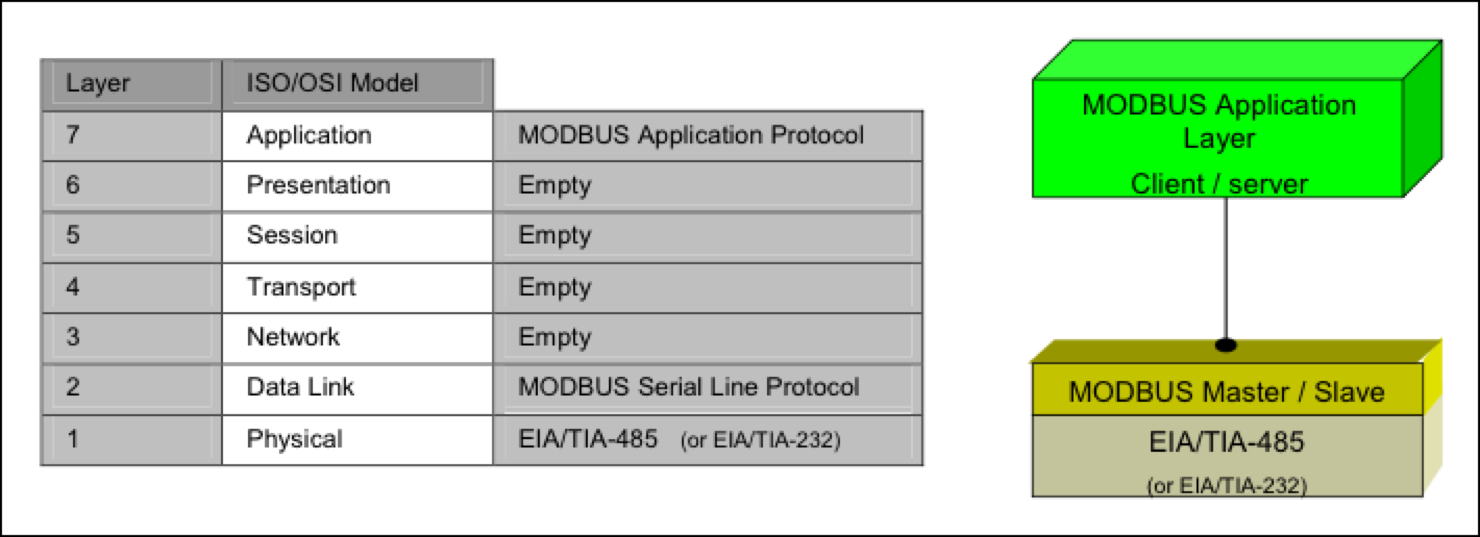
\includegraphics[width=\textwidth]{abbildungen/20160319_modbusosi}
\caption[Die Modbus Kommunikation im OSI-Referenzmodell]{Die Modbus Kommunikation im OSI-Referenzmodell aus \cite[S.~5]{mod06ser}}
\label{fig:modbusosi}
\end{figure}


Das Modbus Application Layer Messaging protocol ist ein Protokoll, dass verschiedene Netzwerke und Bussysteme zur Master/Slave Kommunikationen von verbundenen Geräten nutzen kann \cite[S.~2f.]{mod12}, jedoch übernimmt im Rahmen des Protokolls der Master die Rolle des Clients und die Slaves die Rollen als Server, da der Client alleinig die Anfragen stellt und die Server lediglich auf Anfragen antworten.
Das Modbus Protokoll definiert eine gemeinsame Telegrammstruktur, bezogen auf Inhalte und Rahmen der Nachricht. Damit ermöglicht es die Kommunikation zwischen verschiedenen Geräten innerhalb eines Netzwerks, welche unabhängig von Art und Typ des darunter liegenden Netzwerks sind. Es beschreibt außerdem wie die Kommunikation abläuft, wie der Client eine Anfrage an ein Server stellt und wie diese auf die Anfragen reagieren und antworteten und beschreibt wie Fehler bei der Übertragung entdeckt und darauf hingewiesen werden \cite[S.~2f.]{mod96}.
Die Kommunikation kann dabei über eine serielle Leitung nach EIA 485 sowie über Ethernet Netzwerk erfolgen. Über Gateways, wie in Abschnitt \ref{sec:grundlagenbus} bereits erläutert, kann die Kommunikation auch über verschiedene Typen von Bussystemen oder Netzwerken geschehen \cite[S.~3f.]{mod12}.

Das Modbus Protokoll stellt ein allgemeines Gerüst für Telegramme zur Verfügung, welches in \ref{fig:modbusframe} dargestellt ist.  Die einfache Protocol Data Unit (PDU) enthält die eigentlichen Informationen die ausgetauscht werden sollen und sind daher unabhängig vom Netzwerk oder dem Bussystems. Zu den Informationen gehören die eigentlichen Daten, welche leer sein können oder Daten enthalten die der Slave, in Rahmen von Modbus auch als Server bezeichnet, benötigt, und ein Funktionscode, der ein Byte groß ist und beschreibt welche Art der Aktion Reaktion gefordert ist/wird. Die sogenannte Application Data Unit (ADU) enthält zusätzlich zur PDU weitere Informationen zur Adressierung im Netzwerk und zur Fehlererkennung und ist daher abhängig vom Netzwerk. Der Buszugriff ist damit als Master-Slave geregelt.

\begin{figure}
\centering
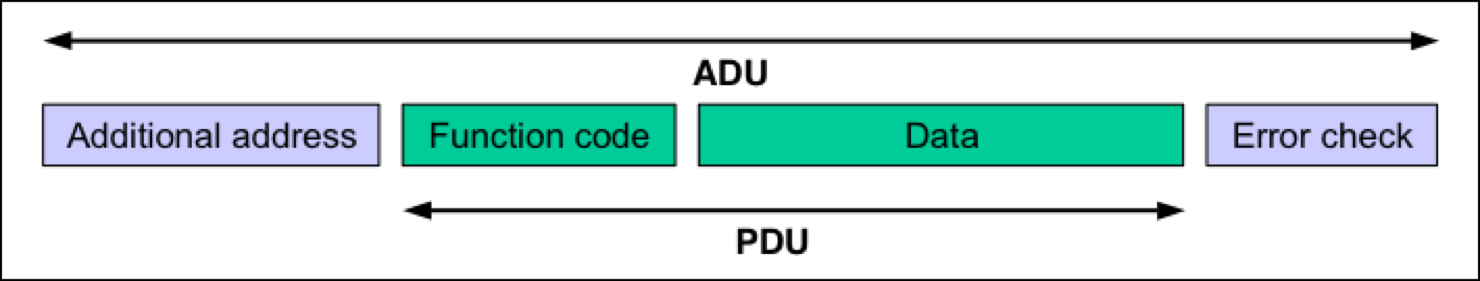
\includegraphics[width=\textwidth]{abbildungen/20160319_Modbusframe}
\caption[Allgemeiner Rahmen für Telegramme nach dem Modbus Anwendungsprotokoll]{Allgemeiner Rahmen für Telegramme nach dem Modbus Anwendungsprotokoll aus \cite[S.~3]{mod12}}
\label{fig:modbusframe}
\end{figure}

Für die Kommunikation wird innerhalb des Masters, der im Rahmen von Modbus auch als Client bezeichnet wird, die Kommunikation durch eine ADU initialisiert. Das genaue Format der ADU wird ist nach Modbus Protokollspezifikation festgelegt. Das Schema einer Transaktion läuft nach dem Prinzip in \ref{fig:modbustransaktion} ab.
Wenn eine ADU fehlerfrei empfangen wurde nutzt der Server das Funktioncode Feld um anzuzeigen, ob seine Antwort ebenfalls eine normale, fehlerfrei Antwort, durch eine einfaches Echo des empfangenen Funktionscodes, ist oder ob ein irgendein Fehler aufgetreten ist durch einen Exception code.
Die Größe der PDU ist grundsätzlich durch die serielle Kommunikation begrenzt auf 256 Bytes, da jedoch noch zwei Bytes für einen Cyclic Redundancy Check und ein Byte für die Server Adresse reserviert werden müssen ist die PDU auf 253 Bytes begrenzt.
Ein weiterer, wichtiger Aspekt ist, dass Modbus die \Gun big-Endian\Gob Codierung/Repräsentation für Daten verwendet verwendet, falls der numerische Wert größer als ein einzelner Byte ist \cite[S.~3ff.]{mod12}. Anhand des Beispielder Uhrzeit kann die Bedeutung der Big-Endian Repräsentation einfach erläutert werden: Die Daten werden so aufgeteilt, dass zunächst die Daten mit der höchsten Wertigkeit, also den Stunden zuerst gesendet werden, anschließend den Minuten und zum Schluss die Sekunden, unabhängig von deren numerischem Wert. Also werden nacheinander die Code 03, 50, 12 empfangen bedeutet dues dass die Uhrzeit 03:50:12 ist. Der interessierte Leser wird für eine weitere Ausführungen auch zu little-Endian Darstellung in \cite{endian05}.

\begin{figure}
\centering
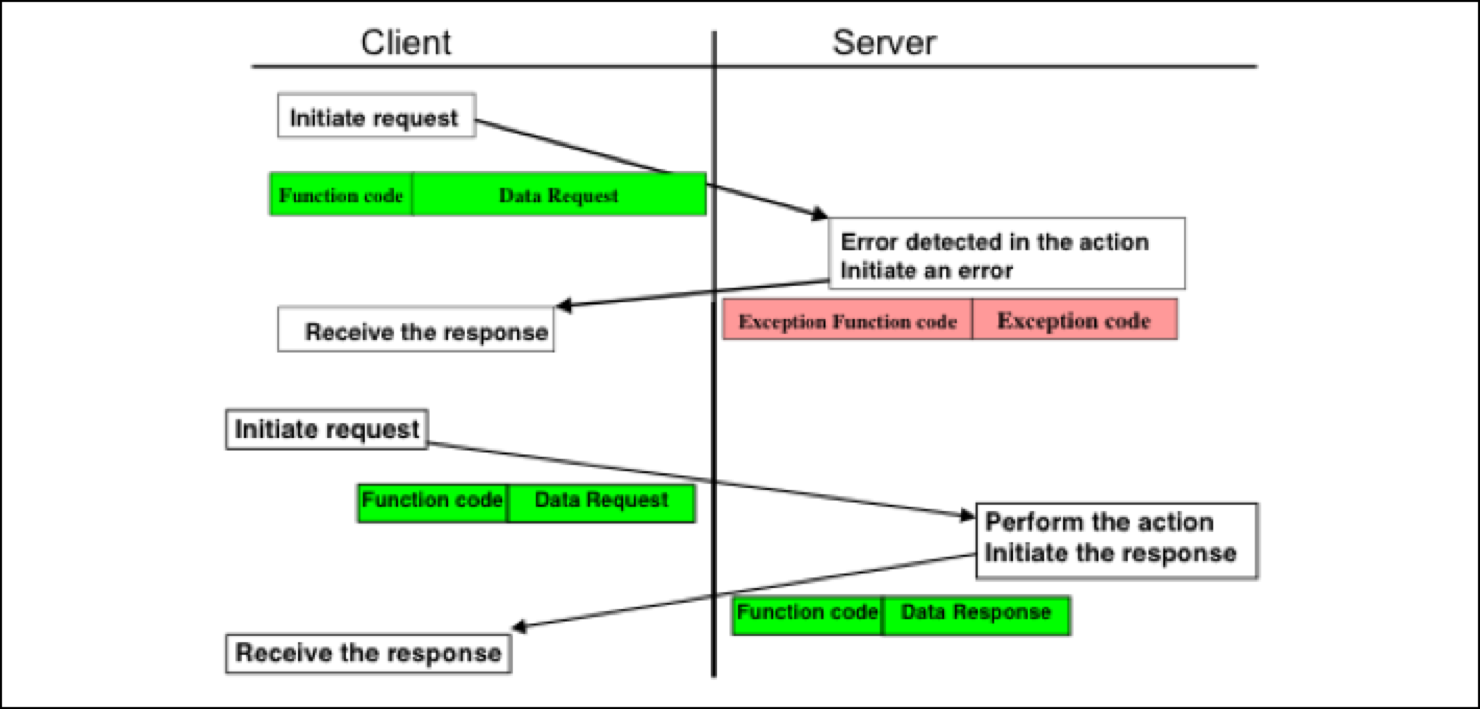
\includegraphics[width=\textwidth]{abbildungen/20160319_modbusclientserver}
\caption[Transaktion mit dem Modbus Protokoll]{Transaktion mit dem Modbus Protokoll nach \cite[S.~4]{mod12}}
\label{fig:modbustransaktion}
\end{figure}

Das Modbus Datenmodell basiert darauf, dass auf die Daten in vier verschiedenen Tabellen mit unterschiedlichen Funktionen und Datenobjekten zugegriffen werden kann:
\begin{itemize}
	\item In die Discretes Input, welche Single Bit Objekte enthält und lediglich gelesen werden kann,
	\item die Coils, welche ebenfalls Single Bit Objekte enthält jedoch gelesen und beschrieben werden darf,
	\item die Input Registers, die Datenobjekte als 16-Bit Wort enthält und wiederum nur gelesen werden kann
	\item und die Holding Registers, dessen 16-Bit Wort Objekte wiederum gelesen und beschrieben werden dürfen.
\end{itemize}

16 bit wort entspricht einer Folge von 16 bits/binärzeichen das also einen dezimalen Zahlenwert zwischen 0 und 65.536. Nach der IEC 61131-3 Norm entspricht es in iim Rechner einem Integer Wert.

Die Daten selbst können auch innerhalb einer Tabelle abgelegt sein, müssen lediglich über die vier angegebenen Tabellen zugreifbar sein, also die Referenz auf die Daten muss gegeben sein, der Rest ist egal. Jede Tabelle besitzt Daten adressiert zwischen 0 und 65535 und ist damit auch nach oben begrenzt was Daten angeht. Welche Daten wo genau stehen, also unter welcher Adresse kann von Gerät zu Gerät unterschiedlich sein und wird vom Gerätehersteller festgelegt. \cite[S.~6ff.]{mod12}

\begin{figure}
\centering
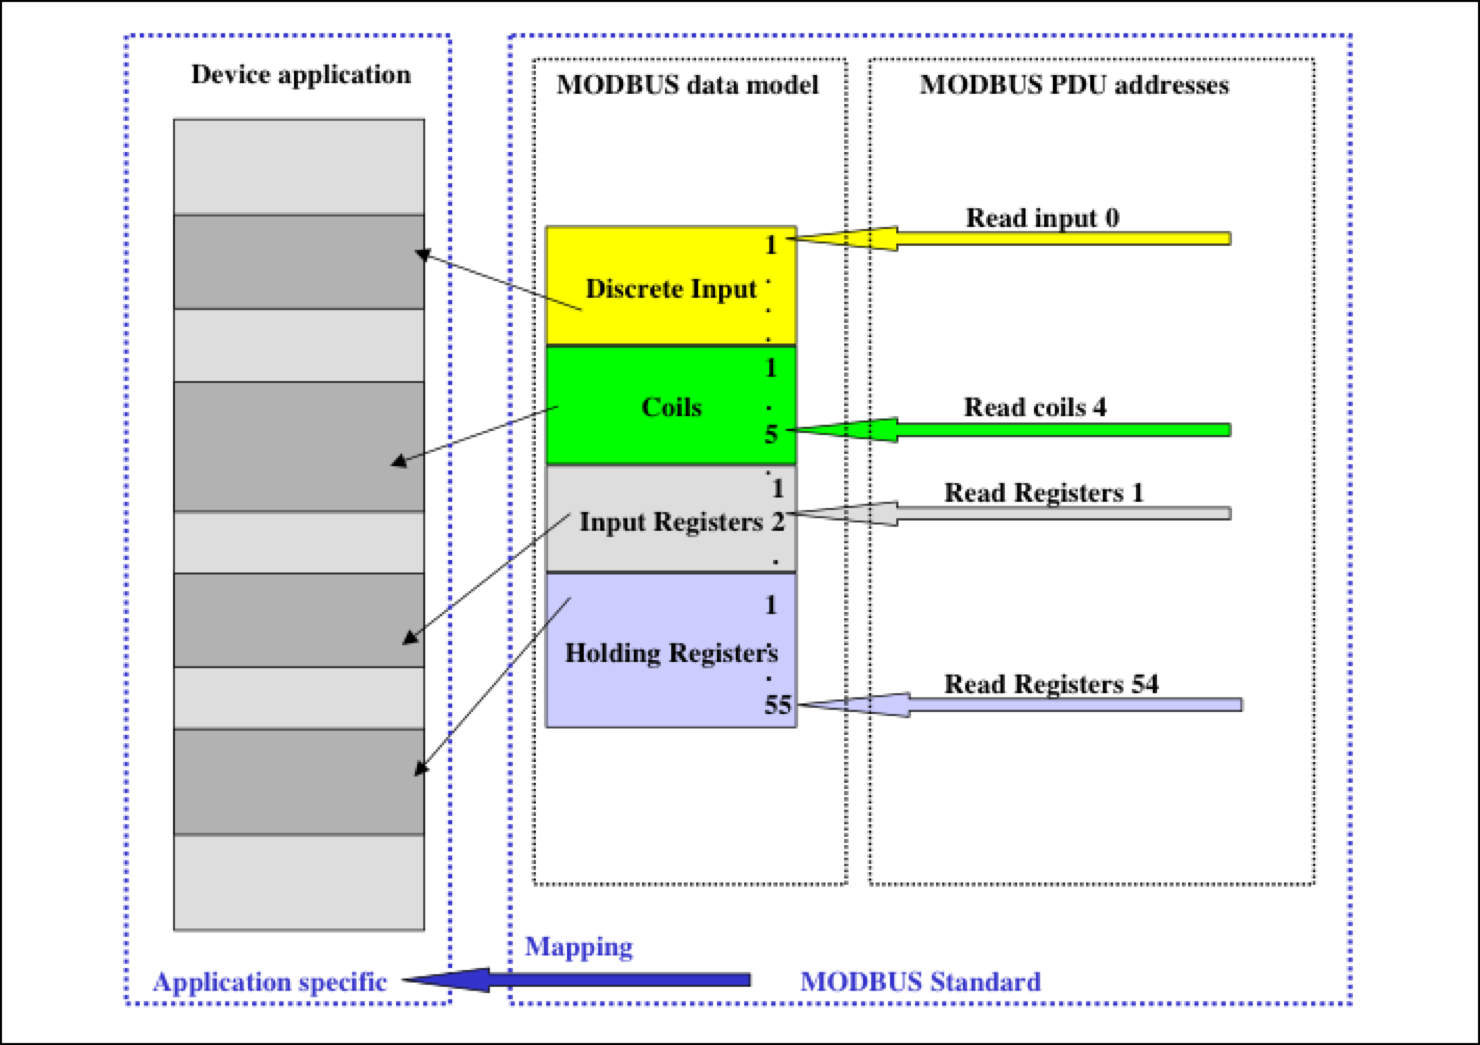
\includegraphics[width=\textwidth]{abbildungen/20160319_modbusadresse}
\caption[Datenmodell und Adressierung nach dem Modbus Protokoll]{Datenmodell und Adressierung nach dem Modbus Protokoll aus \cite[S.~8]{mod12}}
\label{fig:modbusadresse}
\end{figure}

Die Funktionscodes starten bei 1 und können bis 255 genutzt werden und sind wie bereits angesprochen in der PDU enthalten und definieren welche Aktion ein Server ausführen soll. In erster Linie dienen sie dem Datenzugriff in den Tabellen, können aber auch für Diagnosen oder nutzerdefinierte Aktionen benutzt werden. Daher lassen sich die Funktionscodes in drei große Gruppen aufteilen, die öffentlichen, nutzerdefinierbaren und die reservierten Funktionscodes. Die öffentlichen sind wohldefiniert, unique, dokumentiert und sind auf Konformität getestet und sind daher einfach, schnell und sicher nutzbar. Die vom Nutzer definierbaren Funktionscodes können genutzt werden um von den öffentlich bereitgestellten nicht bereitgestellte Funktionen eigens zu definieren/nutzbar zu machen. Die reservierten Codes sind von wenigen Unternehmen, welche an der Entwicklung des Modbus Protokolls beteiligt waren, für deren hinterlassene Produkte reserviert und daher nicht öffentlich nutzbar\cite[S.~10ff.]{mod12}.

Als nächstes folgen die beiden verschiedenen Modbus Over Serial Line Protocol und Modbus Messaging On TCP/IP Protocol

Beim Modbus Over Serial Line Protocol können die Daten über zwei unterschiedliche Modi übertragen werden, der RTU und ASCII Modus. Näheres Der ASCII Modus ist optional und wird in \cite{mod06ser} detailliert beschrieben. Der RTU Modus wird von allen modbusfähigen Komponenten unterstützt und spezifiziert das folgende Format zur Übertragung der einzelnen Bytes: Jede Byteübertragung beginnt mit einem Startbit, auf das zu übertragende Byte, bsetehend aus acht einzelnen Bits, folgt, bevor die Übertragung optional von einem Paritätsbit und einem Stoppbit beziehungsweise lediglich von zwei Stoppbits abgeschlossen wird. Dabei wird jedes zu übertragende Byte als zwei 4-bit hexadezimales Zeichen übertragen\cite[S.~12f.]{mod06ser}. Die Paritätsprüfung ist optional und dient der Fehlerüberprüfung des Telegramms, wie bereits in Abschnitt \ref{sec:grundlagenbus} erläutert.
Der Rahmen eines gesamten Modbus RTU Telegramms besteht aus der Slave Adresse, die für jeden Slave eindeutig ist und zwischen 1 und 247 liegt, und dem Function Code, die jeweils aus einem Byte bestehen. Darauf folgen die eigentlichen Informationen für die 0 bis 252 Bytes vorgesehen sind. Abgeschlossen wird der Rahmen durch ein CRC Feld, dass aus einem CRC Low und einem CRC High byte aufgebaut ist und dazu dient das Telegramm auf Fehler zu überprüfen. Der Ablauf und Vorgang des CRC Checks ist detailliert in \cite{mod06ser} beschrieben. Die Übertragung eines Telegramms erfolgt byteweise, wie zuvor beschrieben. Die Datensicherung findet also durch Parität und CRC auf verschiedenen Ebenen statt.
Die genaue Übertragungszeit eines Bytes und einer Nachricht hängt von der Baudrate ab. Um den Beginn und den Abschluss eines RTU Rahmens eindeutig zu definieren, geschieht dies in Abhängigkeit von der Übertragungsgeschwindigkeit. Zwischen einzelnen Bytes innerhalb eines Rahmens folgt ein stilles Intervall, dass je nach Länge angibt ob das Telegramm beendet ist. Auf eine Intervall kleiner gleich der anderthalbfachen Übertragung eines Bytes folgt eine weiteres Byte. Ist das stille Intervall länger als die dreieinhalbfache Byteübertragungszeit markiert dies das Ende eines Telegramms und den Beginn eines nächsten Telegramms \cite[S.~13]{mod06ser}. Diese Zusammenhänge sind zur Veranschaulichung in \ref{fig:modbusrtu} zusammengefasst.

\begin{figure}
\centering
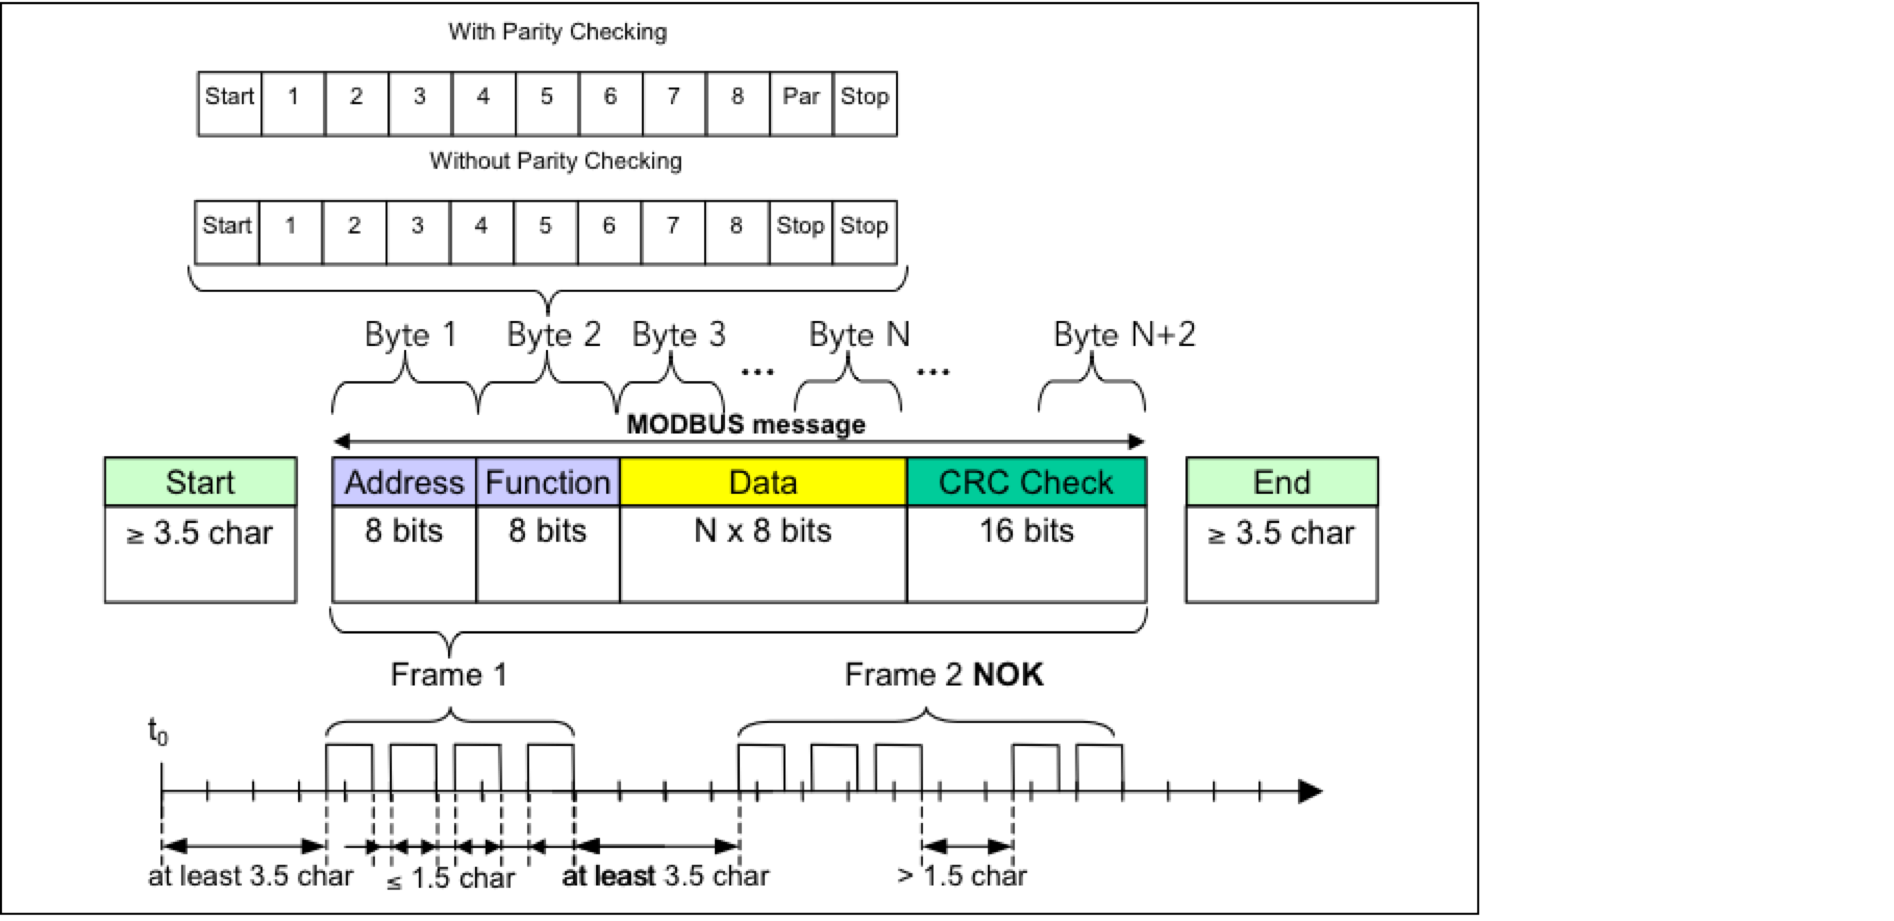
\includegraphics[width=\textwidth]{abbildungen/20160321_rtu}
\caption[Serielle Kommunikation über Modbus RTU]{Serielle Kommunikation über Modbus RTU nach \cite[S.~12f.]{mod06ser}}
\label{fig:modbusrtu}
\end{figure}

Der Implementierungsleitfaden legt auch die Spezifikationen der physikalischen Schicht fest, die nun folgen. Er schlägt vor die EIA 438 Schnittstelle als elektrisches/physikalisches Interface zu verwenden, erlaubt aber auch weiterhin die Implementierung durch die EIA 232 Schnittstelle, beides über ein verdrilltes Leiterpaar. Weiterhin werden die Datenraten von 9.600 und 192.000 bps und eine Even Parität bei der Byteübertragung als Standard festgelegt. Die Standardverdrahtung der Komponenten erfolgt bei beiden elektrischen Standards über ein verdrilltes Leiterpaar und einer gemeinsamen Verbindungsleitung common. Die beiden Leitungen des verdrillten Paares werden mit D1, welche auch als D+ oder A Leitung bezeichnet wird, und D0, welche auch als D- oder B Leitung bezeichnet wird, bezeichnet. Ein Standard Netzwerk besteht aus maximal 32 Teilnehmern, dass durch den Einsatz von Repeatern auch vergrößert werden kann. Außerdem wird die Bus-Struktur als Topologie beschrieben, nach der die einzelnen Komponenten im Netzwerk angeordnet werden, unter der Voraussetzung, dass die Busleitung an beiden Enden durch einen Widerstand von 150 Ohm zwischen der D0 und D1 Leitung abgeschlossen werden \cite[S.~20ff.]{mod06ser}. Die Verbindung der Kabel kann im einfachsten Fall durch Schraubklemmen erfolgen, jedoch können auch genormte mechanische Interfaces, also Standard Steckverbindungen genutzt werden, deren Einsatz und Verkabelung/Anschlüsse in \cite[S.~29ff.]{mod06ser} detailliert beschrieben sind.

XXXXXXXX

Beim Modbus Messaging on TCP/IP Protocol stellt die Möglichkeit zur Verfügung, Geräte, die über ein Ethernet miteinander verbunden sind, über ein Client/Server Modell kommunizieren zu lassen. Des Weiteren erlaubt es dieses Protokoll explizit über Bridges, Gateways oder Router Netzwerke miteinander zu verbinden. Dabei dürfen auch serielle Subnetzwerke zu verbinden und erlaubt auch zwischen diesen Endgeräten die Kommunikation \cite[S.~2f.]{mod06tcp}.
Diese Kommunikationsarchitektur ist auf in \ref{fig:tcparchiktektur} dargestellt. 

\begin{figure}
\centering
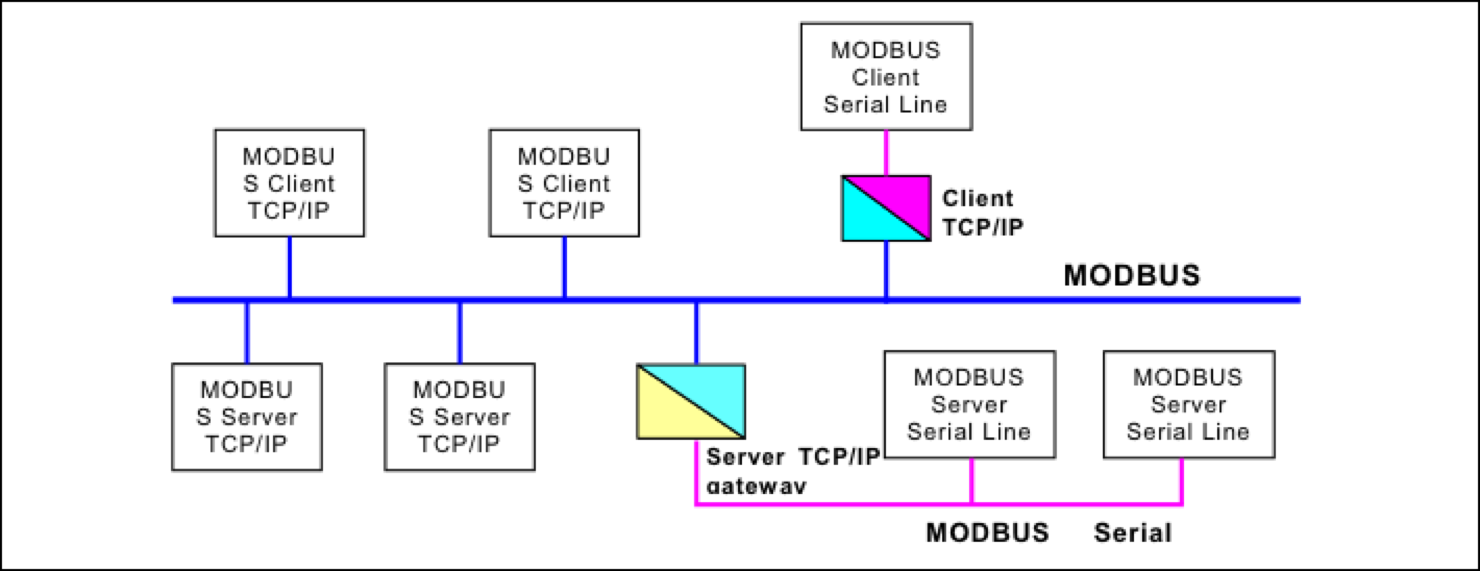
\includegraphics[width=\textwidth]{abbildungen/20160322_tcparchitektur}
\caption[Die Modbus TCP/IP Kommunikationsarchitektur]{Die Modbus TCP/IP Kommunikationsarchitektur aus \cite[S.~4]{mod06tcp}}
\label{fig:tcparchiktektur}
\end{figure}

Außerdem ist eine leicht verschiedne ADU vorhanden, wie in Abbildung REF ADU TCP zu sehen. Modbus Application Protocol Header MBAP Header ist 7 bytes lang und enthält unit identifier ähnlich slave adress/id, adresse für modbus routing, ein bytecount, der die länge des folgenden Telegramms angibt(inklusive Unit identifier und Daten) auch wenn gesplittet, CRC-32 error check, protocol identifier mit modbus 0, transaction identifier vom client, der nur kopiert wird vom server um transaktionen einander zuzuordnen. Alle Kommunikation erfolgt über TCP Port 502 \cite[S.~4f.]{mod06tcp}

\begin{figure}
\centering
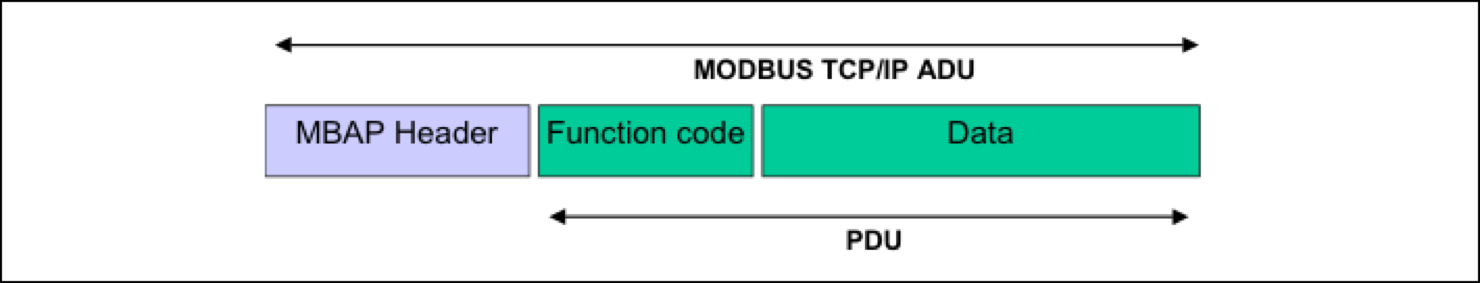
\includegraphics[width=\textwidth]{abbildungen/20160322_tcpframe}
\caption[Angepasster Rahmen für Telegramme nach dem Modbus TCP/IP Protokoll]{Angepasster Rahmen für Telegramme nach dem Modbus TCP/IP Protokoll aus \cite[S.~4]{mod06tcp}}
\label{fig:modbustcpframe}
\end{figure}

Alle Modbus /TCP ADU werden via TCP zum Modbus rgeistrierten Port 502 geschickt.

Modbus tcp Komponenten können sowohl client als auch server interface haben. \cite[S.~7f.]{mod06tcp}

Der Modbus Client erlaubt den Informationsaustausch indem er eine ADU erstellt
Der Modbus Server wartet auf Anfragen über den TCP Port 502

Transmission control protocol TCP und IP ist Internet Protcol. TCP als Transportschicht verbindungsorientiert: Teilt Daten in Datenblöcke, sogeannte Pakete, zum Transport. IP regelt Netzwerkaufgaben, siehe OSI Modell Netzwerkschicht, und versendet die Daten über Telegrammservice und packt den MBAP Header an jedes Paket dran dran. Der Port erlaubt die parallele Nutzung von Ethernet Netzwerken, da er den Übertragungsprozess eindeutig kennzeichnet. Verbindungsorientiert heisst über ein Socket weren zwei prozesse miteinander verbunden und die empfangenen Telegrammen werden/müssen quittiert \cite[S.~16ff.]{schn06}. Der interessierte Leser findet eine deatillierte Beschreibung des Ethernet TCP/IP Standards in \cite{fu03}.


TCP übernimmt Netzwerkmanagement - TCP Management:
Hauptaufgabe ist das connection management. Das managen von Verbindungen kann entweder durch ein Modul erfolgen oder durch die Nutzeranwendung selbst durch die Zugriffsüberwachung der sockets. Der Port 502 ist für Modbus Kommunikation reserviert, jedoch können auch andere Ports genutzt werden falls die Modbusgeräte eine Portkonfiguration unterstützen. Weiterhin wird der Datenfluss und der Einsatz der Netzwerkressourcen überwacht. \cite[S.~7ff.]{mod06tcp}

Generell, Verbindungsmanagement wichtig, da Modbus/TCP Kommunikation zwischen einem Server und einem Clienten eine Verbindung benötigt.
Hinweise gibt der Guide, das die Verbindungen nicht dauernd geöffnet und geshclossen werden und auch mehrere viele Modbus Transaktionen während der Verbindung stattfinden. Außerdem sollte sich auf ein Minimum von Verbindungen beschränkt werden für den gleichen Server. \cite[S.~9f.]{mod06tcp}
Das Nutzer TCP Management umfasst folgende Aufgaben, die aktive und passive Herstellung von Verbindungen sowie das schließen dieser und das festlegen von maximalen Verbindungen \cite[S.~11ff.]{mod06tcp}. Verbindungsherstellung über Ethernet IP, also der eindeutigen Adresse, des Geräts und Portnummer und die Socket Nummer. Der Socket ist ein Endpunkt innerhalb eines Rechners, über den die Kommunikation läuft und der einem Port eindeutig zugewiesen ist \cite[S.~15f.]{mod06tcp} .

Physikalisch bedient sich der Ethernet Schnitstelle also einem normalen Netzwerkkabel.

Diese Kommunikationstechnologie und die verschiedenen Protokolle finden im Rahmen der Anlage in Kapitel dann Anwendung


\section{Technische Grundlagen zur Modellbildung}
\label{sec:grundlagenmodell}
In diesem Kapitel werden die technischen Grundlagen zur Bildung eines mathematischen Modells des Raumes erläutert.
Themrodym systeme
1. HS thermo
Wärmeübertragung

\subsection{Thermodynamische Systeme}
Im Raummodell müssen Energieströme, genauer betrachtet Wärmeströme, untersucht werden. Um dieses thermodynamischen Vorgänge mit Hilfe von Bilanzierungsgleichungen zu beschreiben, folgt zunächst ein kurze Einführung in die Thermodynamische Systembildung nach \cite[S.~11ff.]{ba12}.

\textit{Thermodynamische Systeme} werden durch den zu untersuchenden Raum abgegrenzt. Sie dienen dem Zweck der Bilanzierung von Massen- und Energieströmen und alles was diesen abgegrenzten Raum an den Systemgrenzen umgibt wird als Umgebung bezeichnet. Die begrenzenden Flächen können gedanklicher, physischer oder beider Natur zugleich sein, wichtig ist jedoch das die Systemgrenzen eindeutig festgelegt sind \cite[S.~11]{ba12}.

Anhand der Eigenschaften von den Systemgrenzen lassen sich die thermodynamischen Systeme weiter differenzieren.
Solche Systeme, deren Grenzen undurchlässig für Materie sind, werden als \textit{geschlossene Systeme} bezeichnet und werden durch eine konstante Stoffmenge innerhalb des Systems gekennzeichnet. Die Grenzen eines geschlossenen Systems sind meistens räumlich anhand eines fixen Volumens definiert, können aber auch beweglich sein, wie z.B. das Volumen einer vorgegebenen Stoffmenge unabhängig von dessen räumlicher Ausdehnung \cite[S.~12]{ba12}.

Sind die Grenzen von thermodynamischen Systemen für Materie durchlässig, werden diese als \textit{offene Systeme} bezeichnet. In der Regel werden diese von Stoffströmen durchflossen und durch räumlich festgelegte Grenzen beschrieben. Diese werden in der Literatur auch als \textit{Kontrollraum} oder \textit{Kontrollvolumen} bezeichnet \cite[S.~12]{ba12}.

Ein \textit{abgeschlossenes System} umfasst in der Regel mehrere Systeme oder ein einzelnes System und dessen Umgebung, so dass es zwischen den Grenzen des abgeschlossenen Systems und seiner Umgebung keine Wechselwirkungen gibt. Die Systemgrenzen werden also so gelegt, dass über sie hinweg keine \acrlong{bzw} keine relevanten\footnote{\textit{Relevant} im Sinne von kaum messbarer Fluss und nicht messbare Auswirkung auf das System.} Flüsse von Materie und Energie \cite[S.~13]{ba12}.

Nach der Abgrenzung folgt die \textit{Beschreibung} von thermodynamischen Systemen und dessen \textit{Eigenschaften}. Diese erfolgt durch \textit{Variablen} und \textit{physikalische Größen} die ein System kennzeichnen. Falls die Variablen feste Werte annehmen werden diese als \textit{Zustandsgrößen} bezeichnet, da sie den \textit{Zustand} eines Systems bestimmen \cite[S.~13]{ba12}. Im Rahmen der Modellbildung in Kapitel \ref{chap:modellbildung} ist es ausreichend die Vorgänge und Effekte auf systemischer Ebene zu betrachten, wodurch sich Modelle mit wenigen Variablen und physikalischen Größen beschreiben lassen.

Die Variablen lassen sich in \textit{äußere Größen}, welche den mechanischen Zustand eines Systems beschreiben\footnote{Zum Beispiel die Koordinaten im Raum oder die relative Geschwindigkeit zum Beobachter)}, und \textit{innere Größen} gliedern, welche den thermodynamischen Zustand, also die Eigenschaften der Materie innerhalb der Systemgrenzen, beschreiben\cite[S.13~f.]{ba12}.

Innerhalb der Grenzen eines thermodynamischen Systems, und damit implizit auch für das Raummodell\footnote{Diese Annahme wird im Kapitel \ref{chap:schlussteil} noch überprüft und kritisch hinterfragt werden müssen} wird \textit{Homogenität} angenommen. Dies bedeutet, dass die physikalischen Eigenschaften, wie \acrlong{zb} Temperatur und Druck, sowie die chemische Zusammensetzung an jeder Stelle innerhalb des Systems homogen ist, also die gleiche Ausprägung besitzt \cite[S.15]{ba12}.

Da wir im Rahmen der Modellbildung Zustände betrachten müssen auch deren Änderungen genauer untersucht werden. Die \textit{Zustandsänderungen} eines Systems werden durch Änderungen von Energie oder Materie über dessen Grenzen hinweg bedingt und finden meist im Austausch der Umgebung statt. Während einer solchen Änderung des Systemzustands wird ein Prozess durchlaufen, der eine zeitliche Abfolge von Ereignissen ist. Eine Änderung des Zustands eines Systems mit der gleichen Wirkung kann also durch verschiedene Prozesse bewirkt werden. Daher beschreibt ein \textit{Prozess} nicht nur die Veränderung des Zustands sondern viel mehr die Beziehungen zwischen einem System und seiner Umgebung \cite[S.21~f.]{ba12}.

Ein Prozess kann aber auch innerhalb eines Systems stattfinden, dass heißt ohne äußere Einwirkungen. Dies geschieht zum durch das Aufheben innerer Hemmungen oder dem Wegfall Zwängen von Außen. Diese Prozesse laufen in abgeschlossenen Systemen meist von selbst ab und streben als Ziel einen ausgeglichenen, also homogenen, Endzustand an. \textit{Ausgleichsprozesse} dienen somit dazu, einen \textit{Gleichgewichtszustand} zu erreichen und repräsentieren Wechselwirkungen zwischen verschiedenen Teilen eines abgeschlossenen Systems. Dabei gleichen sich die Zustandsgrößen von einzelnen Subsystemen wie zum Beispiel der Druck oder die Temperatur einander an. Der Gleichgewichtszustand wird also durch die Zustände in den einzelnen Subsystemen bestimmt und ist dadurch charakterisiert, dass ein System diesen Zustand nicht von sich aus sondern nur durch äußere Eingriffe verlässt, zum Beispiel durch eine Veränderungen in der Umgebung. Die Erfahrung lehrt, dass ein System einem Gleichgewichtszustand entgegen strebt, wenn es sich selbst überlassen wird \cite[S.22~f.]{ba12}.
Im Rahmen der Modellbildung in Kapitel \ref{chap:modellbildung} nehmen diese \textit{Ausgleichsprozesse} eine zentrale Rolle ein, weil der Großteil an Änderungen von einzelnen Zustandsgrößen innerhalb des Raumes darauf zurückgeführt werden können. 

\subsection{Erster Hauptsatz der Thermodynamik}
Der erste Hauptsatz der Thermodynamik wird im Folgenden als allgemeiner Energieerhaltungssatz formuliert und anschließend angewendet um eine Energiebilanzgleichung für geschlossene thermodynamische Systeme zu erhalten.

Der erste Hauptsatz der Thermodynamik erweitert den mechanischen Energieerhaltungssatz um die Energieformen Wärme und innere Energie. Er handelt ganz allgemein vom Prinzip der Energieerhaltung und  dient er der Bilanzierung von Systemen \cite[S.~43]{ba12}.

Die Gesamtenergie eines Systems \gls{e} setzt sich zusammen aus der potenziellen \gls{epot} und kinetischen Energie \gls{ekin} wie in der Mechanik und wird durch die innere Energie \gls{u} ergänzt \cite[S.~49]{ba12}:

\begin{equation}
\label{eq:energie}
E := E_{pot} + E_{kin} + U
\end{equation}

Im weiteren Verlauf der Arbeit werden nur ortsfeste Systeme betrachtet die sich dadurch auszeichnen, dass deren potenzielle Energie  \gls{epot} in etwa konstant ist. Weiterhin erfahren sie im betrachteten Intertialsystem Erde auch nur sehr kleine Änderungen in ihrer Geschwindigkeit, weshalb auch die kinetische Energie \gls{ekin} in etwa konstant ist.  Da die Änderungen der mechanischen Energien in Bezug auf die Änderung der inneren Energie sehr klein sind werden im Folgenden nicht weiter betrachtet und die Gesamtenergie eines Systems \gls{e} vereinfacht und lediglich aus der inneren Energie bestehend angenommen.

Die innere Energie hängt von der spezifischen Wärmekapazität \gls{cp}, der Masse eines Systems \gls{msys} und der Temperatur \gls{t} \acrlong{bzw} \gls{T} ab \cite[S.~54]{ba12}:

\begin{equation}
\label{eq:innereenergie}
U := m*c_p*T=m*c_p*t+u_0,~mit~t=T-T_0
\end{equation}

Nach dem Prinzip der Energieerhaltung, kann die Energie eines Systems also weder erzeugt noch vernichtet werden sondern lediglich durch den Energietransport über dessen Grenzen hinweg verändert werden. Daraus ergeben sich folgende qualitative Formen des Energietransports \cite[S.~48f.]{ba12}:

\begin{itemize}
	\item Die Arbeit \gls{w}, die entweder von oder an einem System verrichtet wird, in differentieller Form die Leistung \gls{p}.
	\item Die Wärme \gls{q}, die entweder in das System hinein- oder herausfließt, in differentieller Form der Wärmestrom \gls{qdot}.
	\item Der Transport von Materie, also das Einbringen oder Wegnehmen von Masse \gls{m} eines System, in differentieller Form die Materialflüsse \gls{mdot}.
\end{itemize}

Mit der zuvor getroffenen Annahme, dass die innere Energie der des Systems entspricht, und unter Beachtung der Vorzeichenkonvention, welche besagt dass zugeführte Energie positiv und abgeführte Energie negativ zu bewerten ist, lassen sich die Änderungen der Energie eines Systems mit der folgenden Gleichung quantitativ beschreiben \cite[S.~54]{ba12}:

\begin{equation}
\label{eq:hauptsatz}
\begin{split}
\Delta U & = Q + W + m_{in}*c_{p}*T_{in}-m_{out}*c_{p}*T_{out} \\ ~& \mathrm{beziehungsweise~in~differentieller~Form}\\
\frac{dU}{dt}=\dot{U} & =\dot{Q}+P+\sum\dot{m}_{in}*c_{p}*T_{in}-\sum\dot{m}_{out}*c_{p}*T_{out}
\end{split}
\end{equation}


%Noch einmal überarbeiten

\subsection{Wärmeübertragung}

Wärmeströme spielen bei der Modellbildung in Kapitel \ref{chap:modellbildung} eine wichtige Rolle, daher ist eine genauere Betrachtung dieser unumgänglich und im Folgenden werden die Grundlagen dazu erläutert.

Die Definition von Wärmeübertragung ist nach \cite[S.~1]{bo14} \Gun [...] der Transfer der Energieform Wärme aufgrund einer Temperaturdifferenz. \Gun Die Definition umfasst also einen zuvor beschriebenen Ausgleichsprozess und eine Änderung der inneren Energie eines thermodynamischen Systems.
Die Wärmeübertragung kann nach \textit{Nußelt}\footnote{Beschrieben in seinem Aufsatz \Gun Das Grundgesetz des Wärmeüberganges\Gob , 1915.} grundsätzlich durch zwei verschiedene Arten stattfinden \cite[S.~3f.]{bo14}:

\begin{itemize}
	\item Durch Strahlung, bei der die Übertragung von Wärme ohne stofflichen Träger durch elektromagnetische Wellen zwischen Oberflächen erfolgt. Weil diese Art der Wärmeübertragung keine Relevanz für die weiteren Betrachtungen hat wird er interessierte Leser an dieser auf \cite{bo14} verwiesen der diese Thematik detailliert ausführt. 
	\item  Durch Wärmeleitung, die sich wiederum in die Wärmeübertragung zwischen ruhenden Stoffen, und die Konvektion, die eine Wärmeübertragung zwischen einem ruhenden und einem strömenden Fluid beschreibt, aufteilen lässt. 
\end{itemize}

Die übertragene Wärmemenge ist bei der reinen Wärmeleitung lediglich von den Stoffeigenschaften und der Temperaturdifferenz abhängig, bei der Konvektion hingegen, unabhängig davon ob erzwungen oder frei, hängt sie von der Strömung der Fluide ab. Die Konvektion ist ein Effekt zusätzlich zur reinen Wärmeleitung auftritt und ist im weiteren Verlauf der Arbeit nicht relevant und wird deshalb nicht detaillierter ausgeführt \cite[S.~3f.]{bo14}.
Erfolgt der Wärmetransport stationär, dass heißt er ist von äußeren Anregungen bedingt und unabhängig von der Zeit, lässt er sich qualitativ einfach als konstanter Wärmestrom \gls{qdot} beschreiben und gibt an wie viel Wärme pro Sekunde übertragen wird \cite[S.~5ff.]{bo14}. Der Wärmestrom ist wie zuvor bereits erwähnt von den Stoffeigenschaften abhängig, welche von der Wärmedurchgangszahl \gls{uwert}\footnote{Der U-Wert wurde bis zu der Umstellung auf die europäischen Prüfnormen 2003 als k-Wert bezeichnet und ist unter dieser Bezeichnung noch häufig in der Literatur zu finden \cite[S.1~f.]{sa04}} und der Austauschoberfläche \gls{A}, an der der Wärmeaustausch stattfindet. Typische U-Werte für verschiedene Materialien und Komponenten finden in der einschlägigen Literatur und beziehen sich bei der Übertragung durch eine Wand im europäischen Raum auf die Außenfläche \cite[S.~28]{bo14}. Damit lässt sich der Wärmestrom unter Berücksichtigung der Abhängigkeiten durch die kinetische Kopplungsgleichung quantifizieren \cite[S.~6f.]{bo14}:

\begin{equation}
\label{eq:qdot}
\dot{Q} := u*A*(t_{1}-t_{2})
\end{equation}

Unterschiedliche geometrische Ausprägungen, wie zum Beispiel ein Wärmeaustausch durch eine Wand oder ein Rohr hindurch, finden damit implizit bei der Austauschoberfläche Berücksichtigung.

\section{Technische Grundlagen zur Solar- und Gebäudetechnik}

\subsection{Außenklima und Komponenten}

Der Begriff Außenklima wird häufig im Zusammenhang mit dem Thema Umwelt und deren Einflüsse auf Gebäude gebraucht.  Der allgemeine Begriff des Klimas wird von \cite[S.~295]{ha13} definiert als:
\begin{quote}
\Gun die Summe aller Umweltfaktoren, die unmittelbar oder mittelbar Einfluss nehmen auf die Gesundheit und das Befinden von Menschen und Tieren, auf die Entwicklung von Pflanzen sowie auf den Zustand von Lagergütern, Produktionsverfahren, Maschinen, Apparaten und Bauwerken.\Gob
\end{quote}

Daraus lässt sich ableiten, dass das Außenklima ein Aspekt des Klimas ist und den meteorologischen Umweltzustand außerhalb von Gebäuden, an einem bestimmten, lokalen Ort meint. Abhängig vom Außenklima stellt sich innerhalb von Gebäuden ein Innenklima ein, welches direkten Einfluss auf das Wohlbefinden von Menschen hat und wodurch der mittelbare Einfluss des Außenklimas gegeben ist. Um den Zustand zu beschreiben werden viele Zustandsgrößen herangezogen. Um einen Überblick zu bekommen, lassen sich diese in verschiedene Bereiche gliedern \cite[S.~295f.]{ha13} :
Schall
Licht
Temperatur
und Feuchte
 
Im Hinblick auf die Modellbildung in Kapitel \ref{chap:modellbildung} sind lediglich die Größen zur Beschreibung der Temperatur und des Lichts von Interesse, eine detaillierte Ausführung in die Bereiche Schall und Feuchte und deren Zustandsgrößen ist in \cite{ha13} gegeben.

Je nach Größe des Gebietes wird von einem Regional- bwziehungsweise Makroklima, das große Gebiete umfasst, oder von einem Lokal- beziehungsweise Mikroklima gesprochen, dass kleine Gebiete wie eine Straße oder einen Park umfasst und von deren Besonderheiten abhängig ist. So kann z.B. die Außentemperatur je nach Verschattungsgrad einer Straße lokal erhöht oder erniedrigt sein.
Das Klima folgt in verschiedenen Regionen der Erde bestimmten Charakteristiken, welche sich in Klimazonen zusammenfassen lassen. Die Erde besteht aus vierzehn verschiedenen Klimazonen und in Europa wird von einem Übergangsklima gesprochen \cite[S.~296f.]{ha13}. 

Eine Übersicht der Außenklimakomponenten, die einen Einfluss auf die Gebäudetechnik und damit auch auf die Raumtemperatur haben ist in \ref{fig:aussenklima} gegeben. Für die Modellbildung ist weiterhin eine Quantifizierung der relevanten Größen des Außenklimas in den Bereichen Licht und Temperatur erforderlich. Wie bereits im vorherigen Abschnitt erwähnt, werden Wärmeströme durch Temperaturdifferenzen bedingt, weshalb die Außenlufttemperatur $Hier Symbol$ einen großen Einfluss auf die Raumtemperatur hat und durch Messung quantifiziert werden muss. Des Weiteren werden die lichttechnischen Größen der kurzwelligen direkten und diffusen Strahlung durch die beiden Strahlungsintensitäten $G_{dif}$ und $G_{dir}$ beschrieben, da sie Energie durch einen Wärmestrom in ein System einbringen und damit auch einen Einfluss ausüben.

\begin{figure}
\centering
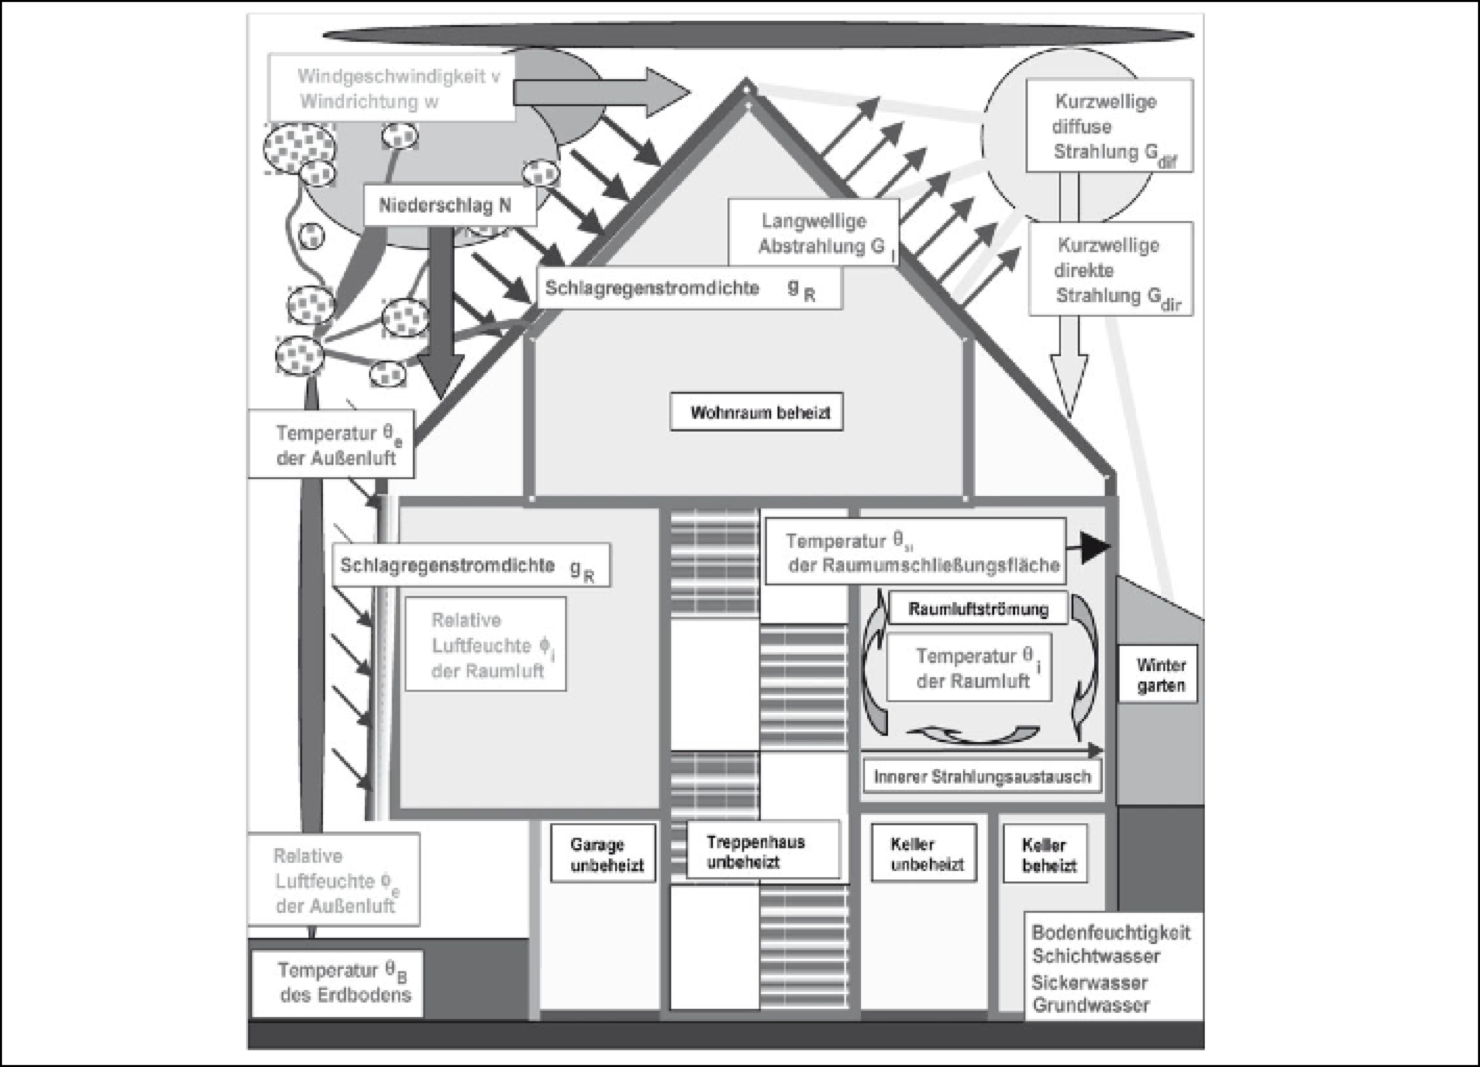
\includegraphics[width=\textwidth]{abbildungen/20160322_aussenklima}
\caption[Komponenten des Außenklimas]{Komponenten des Außenklimas aus \cite[S.~298]{ha13}}
\label{fig:aussenklima}
\end{figure}

\subsubsection{Die Außenlufttemperatur}
Eine Übersicht über die Außenlufttemperatur  


\subsubsection{Sonnenstrahlung}

\cite{therakles13}
\cite[S.~63ff.]{qu11}
\cite[S.~61ff.]{ka13}
\cite[S.~315ff.]{ha13} Bild

Algorithmus nach \cite{re08}

Nutzung Berechnung/Implementierung von \cite{pysolar}

\subsection{Gebäudetechnik Glas und Wärmedurchgangskoeffizienten}
Auf gehts

Glas nach \cite[S.~61ff.]{ha13}
Durchlassgrad nach \cite[S.~604ff.]{ha13}
Transmissionsgrad 



%
% Anlagendesign
%
% @version 1.0
% @author dmayer
% @created 29. Dezember 2015

\chapter{Anlagendesign}
\label{chap:anlagendesign}

\renewcommand{\chapterheadstartvskip}{\vspace*{-0.5cm}}

In diesem Kapitel wird das Design, die Entstehung und Umsetzung der Anlage erläutert. Hierzu wird ausgehend von einer Anforderungsanalyse zunächst das Konzept der Anlage entwickelt, dass anschließend immer weiter konkretisiert wird. Dabei werden die einzelnen Anlagenteile und deren Funktionsweisen detailliert beschrieben und an die realen Einsatzbedingungen angepasst. Abschließend wird die Realisierung und deren Besonderheiten der realen Anlage beschrieben.

\section{Analyse der Anforderungen}
\label{sec:anforderungen}
Um die Anforderungen an die Anlage zu bestimmen, muss zunächst der Zweck/ das Einsatzziel der Anlage untersucht werden. Mit Hilfe der Anlage soll, wie bereits in Kapitel \ref{sec:ziel} erwähnt, auf dem Gebiet der \acrlong{mpc} geforscht und wissenschaftliche Erkenntnisse gewonnen werden (Das Ziel wurde von der Hochschule Karlsruhe in Person von Herrn Adrian Bürger vorgegeben). Um dies zu erreichen, muss die Anlage entsprechend als Entwicklungs- und Anwendungsumgebung für den Einsatz verschiedener Optimalsteuerungen und -regelungen dienen.

Konkret sollen mit dem Einsatz der Anlage die folgende Ziele verfolgt werden:
Der Fokus der wissenschaftlichen Arbeit soll beim Einsatz/Laufen der Anlage besonders auf folgenden Aspekten liegen
\begin{itemize}
	\item Die Einarbeitung in die Thematiken Modellbildung, Optimalsteuerung und \acrlong{mpc} soll ermöglicht/vereinfacht werden.
	\item Das Sammeln von Erfahrungen im Umgang mit der Software, Hardware und deren Schnittstellen sowie verschiedener Methodiken im Bereich \acrlong{mpc} soll stattfinden.
	\item Das Vergleichen von Ergebnissen durch den Einsatz verschiedener Optimalsteuerungen und -regelungen soll möglich sein.
	\item Das Besitzen einer hohen Funktionalität und einer hohen Robustheit gegenüber Fehlern soll erreicht werden, insbesondere um .
\end{itemize}

Aus diesen Einsatzzielen der Anlage lassen sich die konkreten Anforderungen an die Umgebung ableiten. Die Anforderungen sind in Tabelle \ref{tab:anforderungen_umgebung} zusammengefasst.

\begin{table}[H]
\centering
\small
\renewcommand{\arraystretch}{1.3}
\begin{tabularx}{1\textwidth}{m{0.35\textwidth}m{0.58\textwidth}}

\toprule

\textbf{Einsatzziele} & \textbf{Anforderungen} \\

\cmidrule[0.5pt](r{0.25em}){1-1} 
\cmidrule[0.5pt](l{0.25em}){2-2}

Einarbeitung in die Thematiken	& \multirow{2}{\hsize}{Komplexität erwünscht, allerdings nicht zu hoch}  \\

\cmidrule[0.1pt](lr{2em}){1-1} 

Sammeln von Erfahrungen							&					\\

\cmidrule[0.5pt](r{0.25em}){1-1} 
\cmidrule[0.5pt](l{0.25em}){2-2}

Vergleich von Ergebnissen		& Schnell und einfach messbare Reaktionen      \\
\cmidrule[0.5pt](r{0.25em}){1-1} 
\cmidrule[0.5pt](l{0.25em}){2-2}

\multirow{2}{\hsize}{Hohe Funktionalität und Robustheit gegenüber Fehlern} & Einfache Anwendung mit geringer Störanfälligkeit\\
\cmidrule[0.1pt](lr{2em}){2-2} 

 & Einfache, robuste Einzelkomponenten \\
 
\cmidrule[0.5pt](r{0.25em}){1-1} 
\cmidrule[0.5pt](l{0.25em}){2-2}

 & Finanzieller und baulicher Aufwand möglichst minimal \\

\bottomrule
\end{tabularx}
\caption{Übersetzung der Ziele in Anforderungen der Anlage}
\label{tab:anforderungen_umgebung}
\end{table}

Um die Einarbeitung zu vereinfachen sollte die Anlage möglichst wenig Komplexität aufweisen, um die Zusammenhänge und Wechselwirkung zwischen den einzelnen Gebieten und Komponenten möglichst einfach begreifbar zu machen. Da jedoch auch Erfahrungen gesammelt werden sollen, wird ein bestimmtes Maß an Komplexität vorausgesetzt, da diese mit einer wachsenden Zahl von Schnittstellen, verschiedener Soft- und Hardware einhergeht. Dadurch ergibt sich die Forderung nach einem Kompromiss zwischen Verständlichkeit und Komplexität, weshalb ein bestimmtes Maß an Komplexität erwünscht ist.
Das einfache Vergleichen von Ergebnissen soll dadurch ermöglicht werden, dass die Reaktionen/Ergebnisse/Messungen schnell und einfach zu messen sind. Das bedeutet konkret, dass die Anlage zum einen \Gun schnell\Gob eine Reaktion auf Steuerungsimpulse zeigen soll. Zum anderen soll die Reaktion einfach, dass heißt ohne großen technischen und monetären Aufwand und möglichst direkt, messbar sein. Die letzte, sehr wichtige, abgeleitete Anforderung ist eine hohe Funktionalität, um Fehlerquellen außerhalb der Forschung auszuschließen und damit die wissenschaftliche Arbeit zu erleichtern. Entsprechend wird auch eine Robustheit gegenüber Fehlern gefordert, da bei Testeinsätzen von Steuerungen sehr wahrscheinlich auch Fehler passieren sich einstellen und diese keine Schaden an der Anlage verursachen sollen.
Eine weitere Anforderung, unabhängig von den Einsatzzielen oder den technischen Eigenschaften wurde von Seiten der Hochschule vorgegeben: Die Anlage soll mit einem möglichst geringen finanziellen und baulichen Aufwand verbunden sein.



\section{Das Konzept der Anlage}

Trotz einer Vielzahl von technischen Anwendungen, die sich für den im vorangegangenen Kapitel beschriebenen Zweck und dessen Anforderungen eignen, qualifiziert sich  sich besonders eine dafür: Die Steuerung einer Raumtemperatur.

Diese ist mit schnellen als auch einfachen Messungen ohne großen technischen Aufwand verbunden.
, sowie deren Komplexität noch überschaubar ist und mit wenig finanziellem Aufwand verbunden ist. Dadurch ergeben sich zwei potentielle technische Anwendungen: Zum einen die Klimatisierung eines Raumes und zum anderen die Beheizung eines Raumes. Beide weisen ein passendes Maß an Komplexität aufweisen und sich auf Grund ihrer Eigenschaften hervorragend für den Einsatz mit \acrlong{mpc} eignen. Da sich die Raumheizung jedoch mit weniger baulichem und finanziellem Aufwand realisieren lies, wurde letztendlich entschieden diese konkrete Anwendung zum Einsatz zu bringen.


Die Idee der Anlage ist, es mit möglichst wenig Aufwand und Komplexität ermöglichen im ersten Schritt die Raumtemperatur zu erfassen und im nächsten Schritt die Raumtemperatur durch Beheizung zu steuern. Der Bedarf an Komponenten hierfür lässt sich grob in drei verschiedene Gruppen gliedern. Zum einen in die Sensoren zur Ermittlung des Zustandes innerhalb des Raums, der Aktorik zur Beeinflussung des Raumzustandes und einem logischen Controller der die Steuerung der Sensorik und Aktorik übernimmt.
Um den Zustand im Raum zu bestimmen, werden zunächst also Raumtemperatursensoren benötigt. Des Weiteren muss für die Steuerung auch der Zustand der Heizung erfassbar sein, was durch Temperatursensoren am Ein- und Ausgang der Heizung und einen Durchflusssensor überwacht werden soll.
Um den Zustand im Raum beeinflussen zu können, soll der Heizkörper im Raum über einen Aktor am Ventil des Heizkörpers gesteuert werden.
Der logische Controller soll im Rahmen von \acrlong{mpc} Optimalsteuerungspläne berechnen, wofür aureichende Rechenkapazität zur Verfügung stehen muss -- da Optimierung gradientenbasiert erfolgt -- weshalb diese Aufgabe von einem Rechner übernommen werden soll.

Somit gilt es eine Schnittstelle zu finden um eine Zusammenarbeit aller Gruppen zu ermöglichen.

Die Anforderungen an die Anlage wurden bereits in Kapitel \ref{sec:ziel} erläutert und sollen nun bei der Planung Beachtung finden.
Bei der Konzipierung müssen neben den Anforderungen, welche in Kapitel \ref{sec:ziel} , weitere Überlegungen angestellt werden um eine reibungslose Zusammenarbeit der verschiedenen Anlagenteile gewährleisten zu können. (Größtmögliche Kompatibilität)
Dazu werden zunächst die Restriktionen der einzelnen Anlagenteile
Die Optimalsteuerung 
Das Hauptaugenmerk bei der Konzipierung liegt deshalb auf der Kompabilität und möglichst großen Einfachheit der einzlenen Komponenten der Heizungstseuerung. 


\section{Räumliche Gegebenheiten}
Einen ersten Überblick der räumlichen Gegebenheiten sowie deren Lage ist auf der Skizze in Abbildung \ref{fig:skizzek004a} gegeben. Der Raum, dessen Temperatur geregelt werden soll, befindet auf dem Campus der Hochschule Karlsruhe im Gebäude K und ist ein Büro für wissenschaftliche Mitarbeiter. 
Wie in Abbildung \ref{fig:skizzek004a} zu sehen, ist der Raum von 4 Wänden quaderförmig umgeben. Die beiden dickeren Wände, die grob nach Süden und Westen ausgerichtet sind, grenzen an die Außenumgebung. Die anderen beiden Wände, sowie Decke und Boden, grenzen an anderen Räume im Gebäude. Die Ein- und Ausgangstüre befindet sich in der nordöstlichen Ecke an der Ostwand. Die nach Süden ausgerichtete Außenwand besitzt eine hohe Fensterfront. Außerdem ist unterhalb des Fensters ein Heizkörper installiert, der bisher mit einen Thermostat ausgestattet ist, der die Heizung über ein Ventil  steuert.
Da der Raum ein Büro ist, sind Innerhalb des Raumes nicht nur eine Büroausstattung aus Schreibtischen und Schränken auch sechs Rechner sowie deren Nutzer zu finden/berücksichtigen.

\begin{figure}
\centering
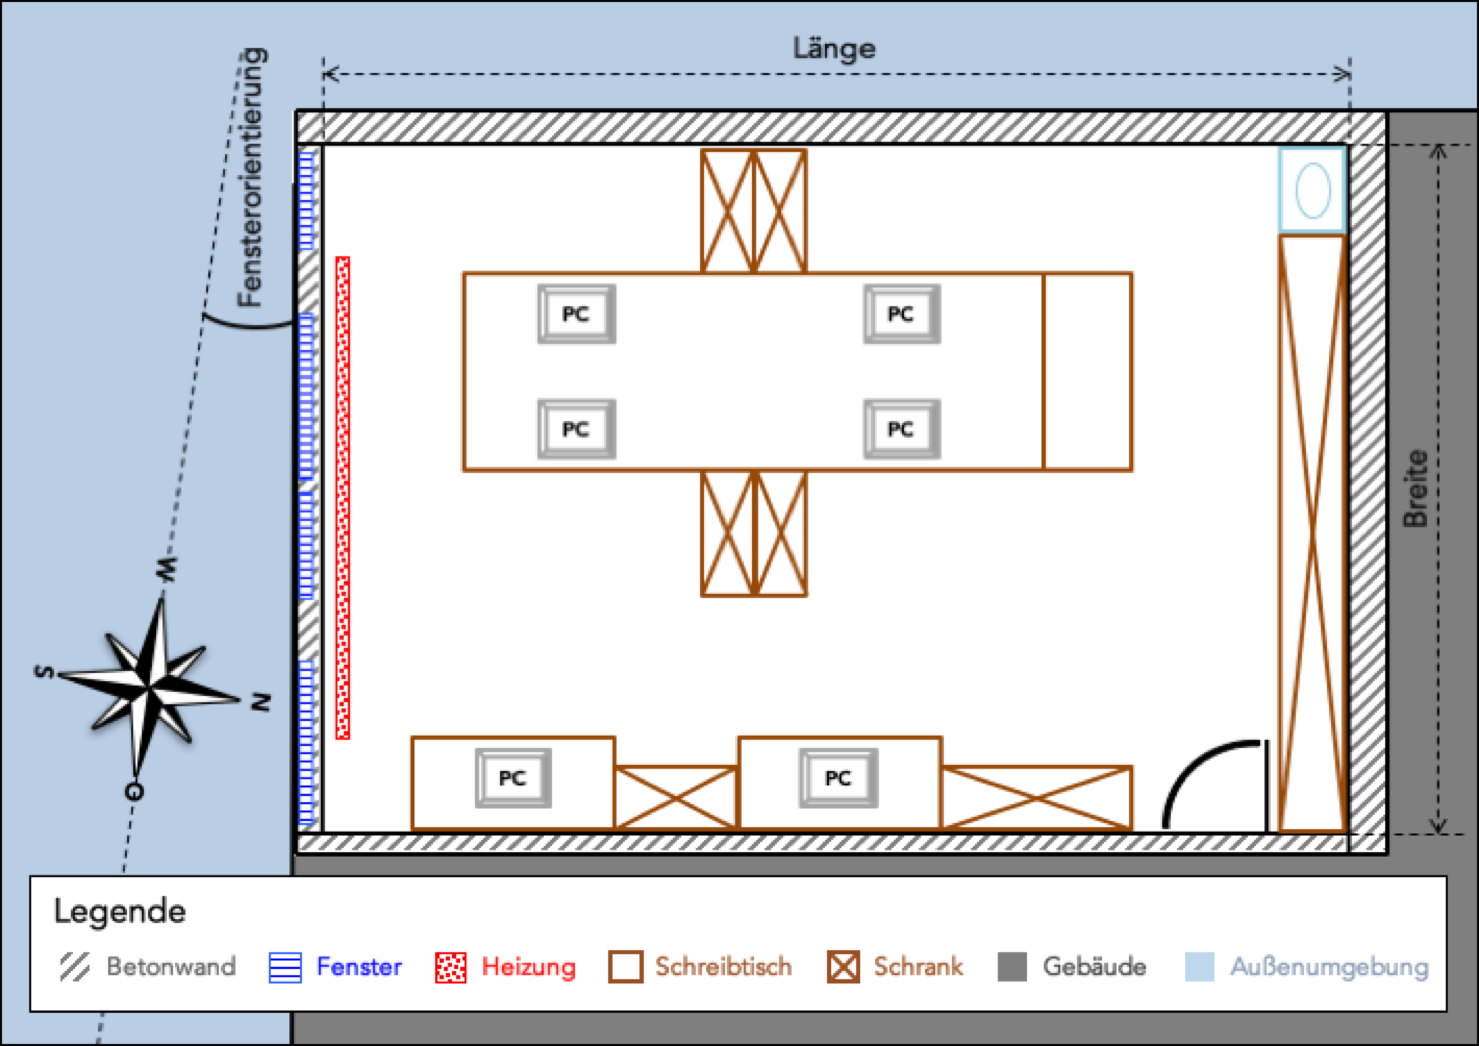
\includegraphics[width=\textwidth]{abbildungen/20160102_k004a}
\caption[Raumskizze K004A vom K Gebäude der Hochschule Karlsruhe -- Technik und Wirtschaft]{Raumskizze K004A vom K Gebäude der Hochschule Karlsruhe -- Technik und Wirtschaft}
\label{fig:skizzek004a}
\end{figure}

\section{Konzipierung der Steuerung}
Die Steuerung der Anlage 
Für die Berechnung von Optimalsteuerungsplänen wird 
Die Optimalsteuerung stellt in diesem Fall den begrenzenden Faktor dar, da die Optimierungsumgebund CasADi für dynamische Systeme nur unter JModelica.org läuft. Daher wird darauf aufbauend das benötigte Modell für die MPC in Modelica gebildet unter Berücksichtigung der Restriktionen bezüglich JModelica. Die gemeinsame Schnittstelle beider ist Python, übder die damit auch die Kommunikation mit den Hardwarekomponenten der Heizungstseurung erfolgen muss/soll.

Bild Hardware ---- Software   Interface Python, da Software darauf angewiesen ist.



Das Hauptaugenmerk bei der Planung liegt deshalb auf der Kompabilität und möglichst großen Einfachheit der einzlenen Komponenten der Heizungstseuerung. 

Die Optimalsteuerung stellt in diesem Fall den begrenzenden Faktor dar, da die Optimierungsumgebund CasADi für dynamische Systeme nur unter JModelica.org läuft. Daher wird darauf aufbauend das benötigte Modell für die MPC in Modelica gebildet unter Berücksichtigung der Restriktionen bezüglich JModelica. Die gemeinsame Schnittstelle beider ist Python, übder die damit auch die Kommunikation mit den Hardwarekomponenten der Heizungstseurung erfolgen muss/soll.

Bild Hardware ---- Software   Interface Python, da Software darauf angewiesen ist.

\section{Umsetzung der Anlage}


\section{Inbetriebnahme und Ansteuerung der Anlage}

%
% Anlagendesign
%
% @version 1.0
% @author dmayer
% @created 29. Dezember 2015

\setchapterpreamble[o]{%
\dictum[--- \textsc{Norbert Wiener}]{\Gun Das beste Modell für eine Katze ist eine Katze; möglichst dieselbe Katze. \Gob}}
\renewcommand{\chapterheadstartvskip}{\vspace*{2cm}}

\chapter{Modellbildung des Raumes}
\label{chap:modellbildung}

\lstinputlisting[language=Modelica, linerange=194-20, label=lst:room]{listings/room_model_listing.mo}

Ziel dieses Kapitels ist es, ein hinreichend exaktes Modell zur Berechnung der Raumtemperatur, basierend auf den thermodynamischen Prozessen mit dessen Umgebung und der Anlage aus Kapitel \ref{chap:anlagendesign}, zu bilden, um damit und unter Zuhilfenahme der Anlage Modellpräditive Regelung zu ermöglichen.
Dazu wird zunächst ein einfaches Grundmodell für einen hypothetischen Raum gebildet, dass anschließend schrittweise an den bestehenden Raum erweitert angepasst wird, bis eine die Qualität des Modells ausreichend ist.

\section{Anforderungen an das Raummodell}
Da MPC die Lösung von Nichtlinearen Gleichungssystemen erfordert wird ein erhöhter Rechenbedarf benötigt. Daher sollte das Modell so einfach wie möglich gehalten werden. Die Krux liegt also darin, einen geeigneten Kompromiss zwischen Komplexität und Genauigkeit des Modells zu finden, der eine sinnvolle MPC Regelung ermöglicht.
Des Weiteren werden gradientenbasierte Ableitungen bei der Optmierung/Lösung des LGS generiert weshalb auch keine Unstetigkeiten im Modell vorkommen dürfen.
Die triviale Aufgabe ist die hinreichend genaue Beschreibung der Realität bzw realen Vorgänge.
Damit eine Steuerung mit Hilfe von Modellprädiktiver Regelung möglich ist, darf das Modell keine hohe Kompliziertheit aufweisen und sollte durch möglichst wenig Gleichunge trotzdem ein möglichst genaues Abbild der Realität abbilden.
Das Modell soll zunächst so simpel wie möglich gestaltet werden um eine Optimierung mit Hilfe von MPC zu ermöglichen. Dessen Verfahren zur Optimierung sind gradientenbasiert und erfordern damit die Erzeugung von stetigen Ableitungen bis zum zweiten Grad. Daher soll die Komlpexität des Modells zunöchgst sehr gering gehalten werdeen und dann Stück für Stück erhöht werden und die damit die Geanuiogkeit des modells erhöht werden

\section{Das Grundmodell des Raumes}

Um ein möglichst einfaches Grundmodell zu erhalten, wird zunächst ein hypothetischer Raum betrachtet, der in \ref{fig:grundraum} dargestellt ist. Dieser Raum bildet zusammen mit der ihn umgebenden Luft ein abgeschlossenes thermodynamisches System, wie in Kapitel \ref{sec:grundlagenmodell} beschrieben. Der Raum ist selbst mit Luft gefüllt und wird zu allen sechs Seiten hin durch Wände begrenzt. Damit bildet der Raum ein geschlossenes System, da keine Massenströme über die Grenzen hinweg fließen können. An den Grenzflächen kann also lediglich Wärme zwischen der Luft außerhalb und innerhalb des Raumes ausgetauscht werden. Des Weiteren wird eine homogene Temperatur innerhalb des Raumes und der Umgebung angenommen, was einem eingeschwungenen Zustand/Gleichgewichtszustand in der Realität entspricht. Diese Annahme ist jedoch noch zu überprüfen.

\begin{figure}
\centering
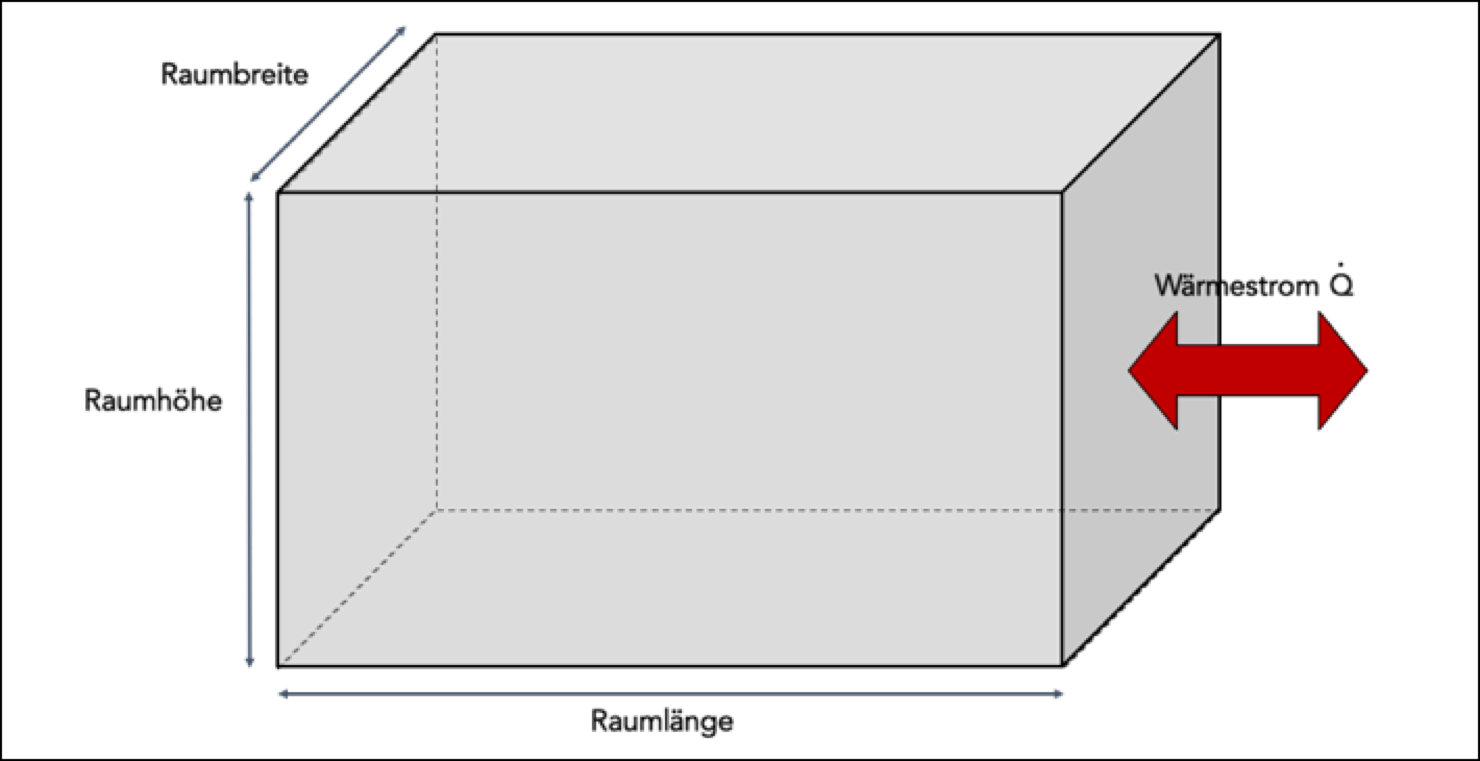
\includegraphics[width=\textwidth]{abbildungen/20160316_grundraum}
\caption{Grundmodell eines Raumes}
\label{fig:grundraum}
\end{figure}

Zur Bestimmung der Raumtemperatur muss, ausgehend von einer initialen Raumtemperatur und der Umgebungstemperatur, der Ausgleichsprozess zwischen Raum und Umgebung untersucht werden, konkret der ausgetauschte Wärmestrom. Um diesen nach \ref{eq:qdot} zu berechnen, müssen zunächst die verschiedene modellrelevanten Eigenschaften des Raumes durch physikalische Größen und Variablen beschrieben werden. Zur Berechnung der Austauschoberfläche wird die Raumbreite, -länge und -höhe benötigt und weiterhin sind der U-Wert einer Betonwand, die spezifische Wärmekapazität und Dichte von Luft für die Bestimmung des Wärmestroms relevant.

Diese modellrelevanten Eigenschaften sind allesamt mit ihren Zahlenwerten in Tabelle \ref{tab:eigenschaften_raum} zusammengefasst.

\begin{table}[H]
\centering
\small
\renewcommand{\arraystretch}{1.3}
\begin{threeparttable}
\begin{tabularx}{1\textwidth}{p{0.5\textwidth}m{0.2\textwidth}m{0.18\textwidth}}
\toprule
\textbf{Modellrelevante Eigenschaften} & \textbf{Wert} & \textbf{Einheit} \\
\cmidrule[0.5pt](r{0.25em}){1-1} 
\cmidrule[0.5pt](l{0.25em}){2-2}
\cmidrule[0.5pt](l{0.25em}){3-3}

Raumbreite & 7,81\tnote{1)} & $[m]$ \\ 
\ccol Raumlänge & \ccol 5,78\tnote{1)} & \ccol $[m]$ \\
Raumhöhe & 2,99\tnote{1)} & $[m]$ \\
\ccol Wärmedurchgangskoeffizient & \ccol 2\tnote{2)} & \ccol $[\frac{W}{m^{2}*K}]$\\
Spezifische Wärmekapazität von Luft & 1.000\tnote{3)} & $[\frac{J}{kg*K}]$\\
\ccol Dichte von Luft & \ccol 1,25 \tnote{3)} & \ccol $[\frac{kg}{m^{3}}]$\\
\bottomrule
\end{tabularx}
\begin{tablenotes}[]\footnotesize\singlespacing\setlength\labelsep{0pt}
\item[1)] Werte durch eigene Vermessung des Raumes K004b vom 07.12.2015
\item[2)] Schätzwert, geschätzt nach \cite[S.~409]{re14} mit Richtwerten aus \cite[S.~194ff.]{re14}
\item[3)] Tabellenwert aus \cite[S.~139]{ha13}
\end{tablenotes}
\end{threeparttable}
\caption{Eigenschaften des Raummodells}
\label{tab:eigenschaften_raum}
\end{table}

Erfolgt nun die Bilanzierung des Raumes mit Hilfe des ersten Hauptsatzes der Thermodynamik nach \ref{eq:hauptsatz} und die Berechnung der inneren Energie des Raumes nach \ref{eq:innereenergie} ergibt sich folgendes, einfaches Gleichungssystem zur Bestimmung der Raumtemperatur im Grundmodell in Modelica:

\begin{lstlisting}[language=Modelica, label=lst:grundraum]
equation
   /* calculate room volume */
   room_volume = room_length * room_height * room_breadth;
   /* calculate room mass */
   room_mass = room_volume * rho_air;
   /* calculate surface of heat exchange */
   exchange_surface = 2 * (room_length * room_breadth) + 2 * (room_length * room_height) + 2 * (room_breadth * room_height);
   /* calculate inner energy*/
   room_u = room_mass * cp_air * room_temperature;
   /* calculate derivative of the inner energy */
   der(room_u) = environment_qdot;
   /* calculate heatflow between room and environment */
   environment_qdot = u_wall * exchange_surface * (environment_temperature - room_temperature);
\end{lstlisting}

Damit ist das Grundmodell für einen Raum in Modelica beschrieben, das im Folgenden schrittweise erweitert wird um der Realität genpüge zu tragen.

\section{Modellerweiterung durch Berücksichtigung realen Umgebung}

Im nächsten Schritt wird das Raummodell an die realen, räumlichen Gegebenheiten des Raums K004b angepasst. In der \ref{fig:skizzek004a} wird deutlich, dass der Raum lediglich zwei Außenwände besitzt, die an die Umgebungsluft grenzen: Die Wände in Richtung Süden und Westen. Die anderen beiden Wände, sowie die Decke und der Boden, grenzen an weitere Gebäudeteile des K-Gebäudes. Der Raum ist nach wie vor ein geschlossenes System und bildet zusammen mit dem umgebenden K-Gebäude und der Umgebung wiederum ein abgeschlossenes System. Jedoch können nun verschiedene Wärmeströme zwischen dem Raum und der Außenumgebung sowie dem Raum und dem K-Gebäude ausgetauscht werden. Aufgrund der Relation der Wärmeströme im Gegensatz zur großen Energie des K-Gebäudes und der Umgebung, wird der Erwärmungs- bzw Abkühlungseffekt durch den Wärmestrom mit dem Raum vernachlässigt und von konstanten, homogenen Temperaturen innerhalb der Umgebung und des K-Gebäudes ausgegangen.

Durch diese Erweiterung des Modells wird die gesamte Austauschoberfläche zum Wärmeaustauschs aufgeteilt in die Austauschoberfläche mit der Umgebung und die Austauschoberfläche mit dem K-Gebäude, um die Wärmeströme separat berechnen zu können. Des Weiteren werden im Modell die Temperatur der Außenumgebung und die Temperatur innerhalb des K-Gebäudes als externe Steuergrößen berücksichtigt. Das Gleichungssystem des Grundmodells in \ref{lst:grundraum} erweitert sich also um folgende Änderungen:

\begin{lstlisting}[language=Modelica,label=lst:raumeins]
equation
   [...]
   /* calculate surface of heat exchange with environment */
   environment_exchange_surface = room_length * room_height + room_breadth * room_height;
   /* calculate surface of heat exchange with the remaining building */
   building_exchange_surface = 2 * (room_length * room_breadth) + room_length * room_height + room_breadth * room_height;
   /* calculate derivative of the inner energy */
   der(room_u) = environment_qdot + building_qdot;
   /* calculate heatflow between room and environment */
   environment_qdot = u_wall * environment_exchange_surface * (environment_temperature - room_temperature);
   /* calculate heatflow between room and building */
   building_qdot = u_wall * building_exchange_surface * (building_temperature - room_temperature);
\end{lstlisting}


\ref{lst:room}

Die Abgrenzung bzw Wahl der Grenzen zur Bilanzierung eines thermodynamischen Systems erfolgt nach dem gesuchten Zustand und der gesuchten Zustandsgröße, der Raumtemperatur im Raum K004b. Der gesucten hießt zu berechnenenden/unbekannten

Zum einen in den zu untersuchenden Raum, der durch die Aussenwände des Raumes begrenzt wird und innerhalb dessen Grenzen die zu betsimmende Raumtemperatur vorherrscht. Zum anderen die Teilsysteme Gebäude und die Umgebung, innerhalb deren Grenzen jeweils auch eine chrakterisierende Temperatur vorherrscht. Die Systemgrenzen des Raumes werden als geschlossen angesehen, dass heißt das Öffnen und schließen von Fenstern und Türen wird nicht explizit berücksichtigt sondern kann nur nur implizit als Störgröße berücksichtigt werden. Die Grenzen zwischen den Teilsystemen 


\section{Erweiterung durch Sonneneinstrahlung}


\section{Erweiterung durch Heizkörper}

\section{Validierung des Modells}

\section{Anpassung des Modells mit Parameterschätzung}
%
% Schlussbetrachtung
%
% @version 1.0
% @author wipatrick
% @created 22. November 2015
% @edited 

\setchapterpreamble[o]{%
\dictum[--- \textsc{Jack Dangermond}, \emph{Esri}]{\Gun Knowing where things are, and why, is essential to rational decision making.\Gob}}
\renewcommand{\chapterheadstartvskip}{\vspace*{3cm}}

\chapter{Schlussbetrachtung}
\label{chap:schlussteil}
\renewcommand{\chapterheadstartvskip}{\vspace*{-0.5cm}}

\section{Fazit}
\label{sec:zusammenfassung}

%\blindtext

\section{Ausblick und Ansatzpunkte für weitere Arbeiten}
\label{sec:ausblick}

Welchge art der Verwendung?
MPC mit JModelica.org also deren mpc klasse
eigene in casadi
etc?

%----------------------------------------------------------------------------------------------------------------------
% Anhang 
%----------------------------------------------------------------------------------------------------------------------
%\appendix
\chapter{Modelle, Programme, Messdaten}
\label{att:cd}
Auf der beiliegenden CD befinden sich:
\begin{itemize}
	\item die Modelle
	\item Skripte zur Parameterschätzung
	\item Messdaten
\end{itemize}

\newpage


\chapter{Modelle}
%Aufteilen in einzelne Modelle
\section{Raummodell}
\label{att:raummod}
\lstinputlisting[language=Modelica]{listings/room_model_backup.mo}
%
%
%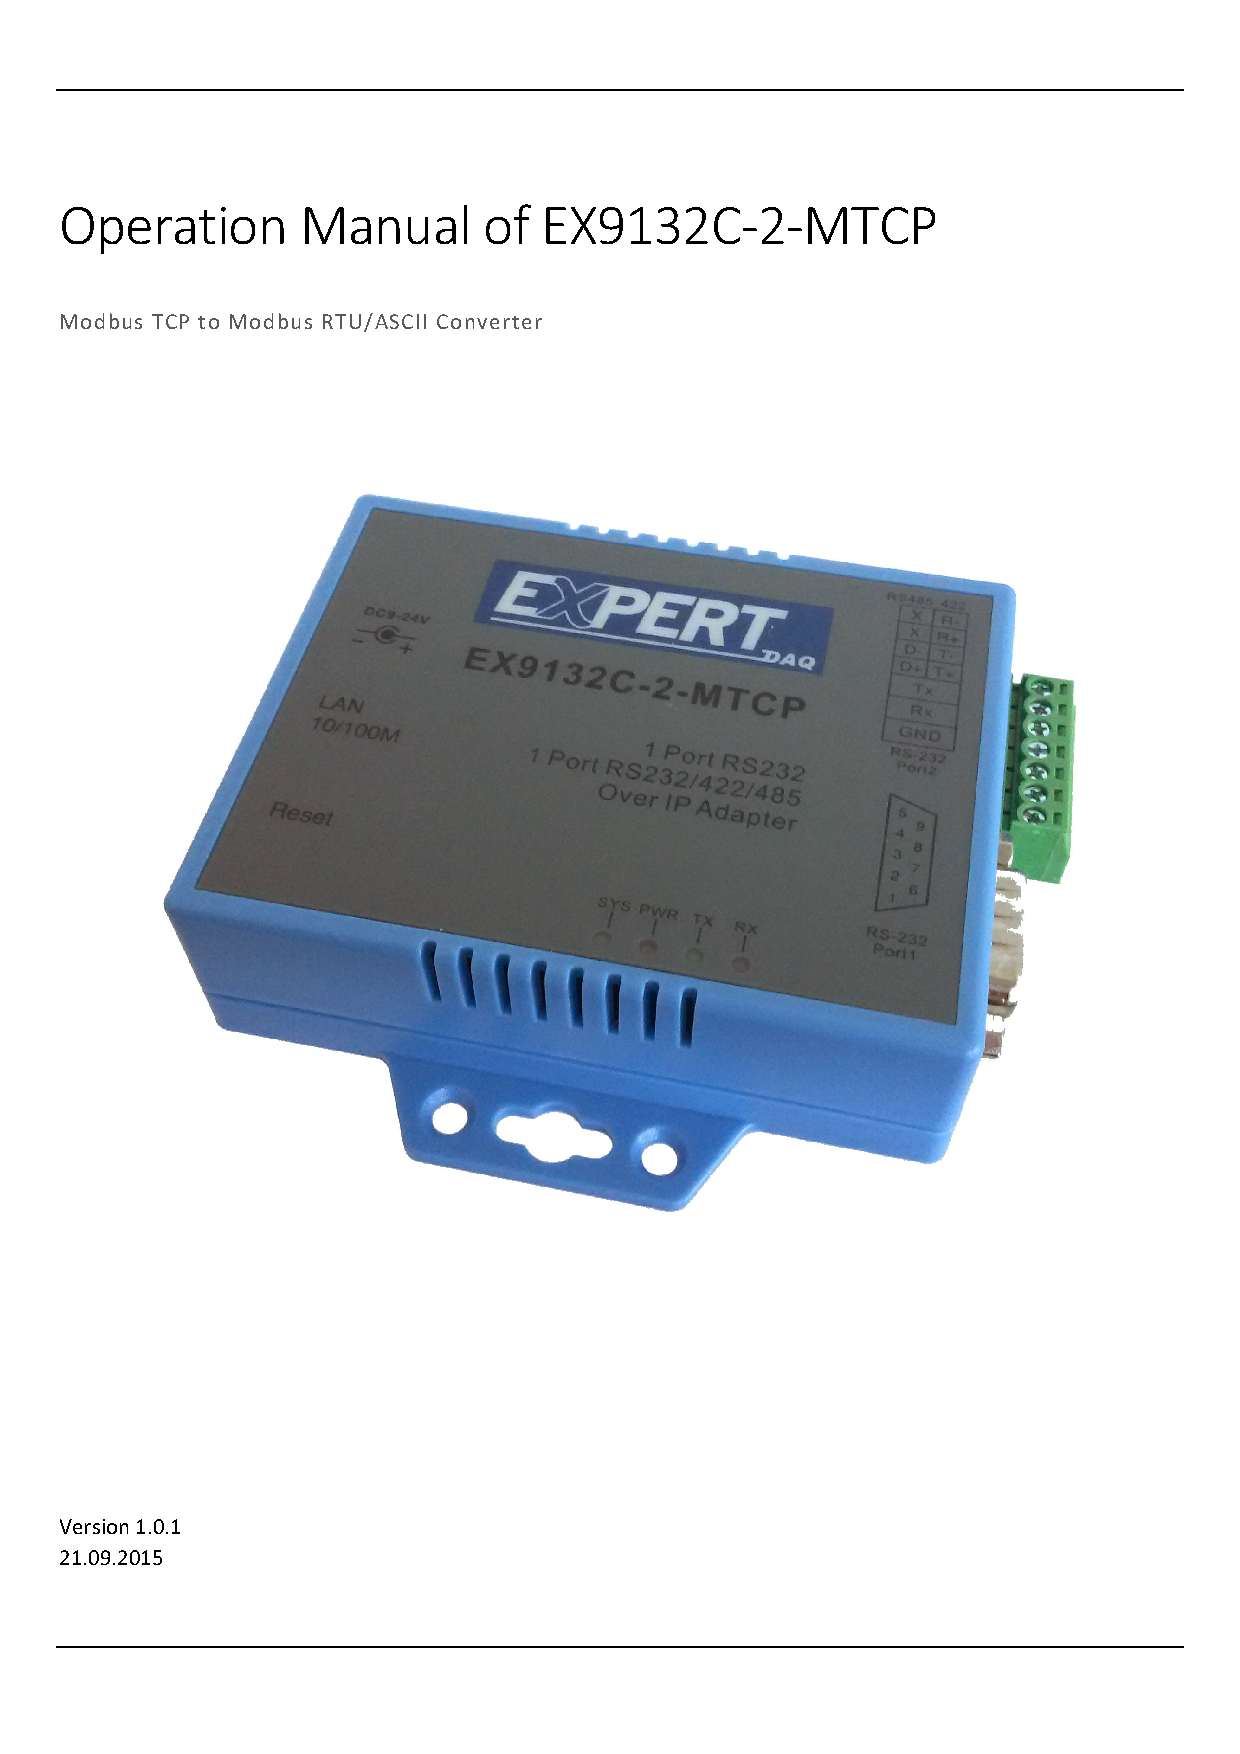
\includepdf[pagecommand={\chapter{Datenblätter}\section{EX9132C-2-MTCP Gateway von ExpertDAQ}\label{att:ex9132}}, pages={1}, scale=0.7, offset=0.1cm -3cm]{anhang/ex9132}
%\includepdf[pages={4-7}, scale=0.8]{anhang/ex9132}
%\includepdf[pages={10}, scale=0.8]{anhang/ex9132}
%\includepdf[pages={17-20}, scale=0.8]{anhang/ex9132}
%\includepdf[pages={22-23}, scale=0.8]{anhang/ex9132}
%
%\includepdf[pages={2}, scale=0.8]{anhang/rtm1}
%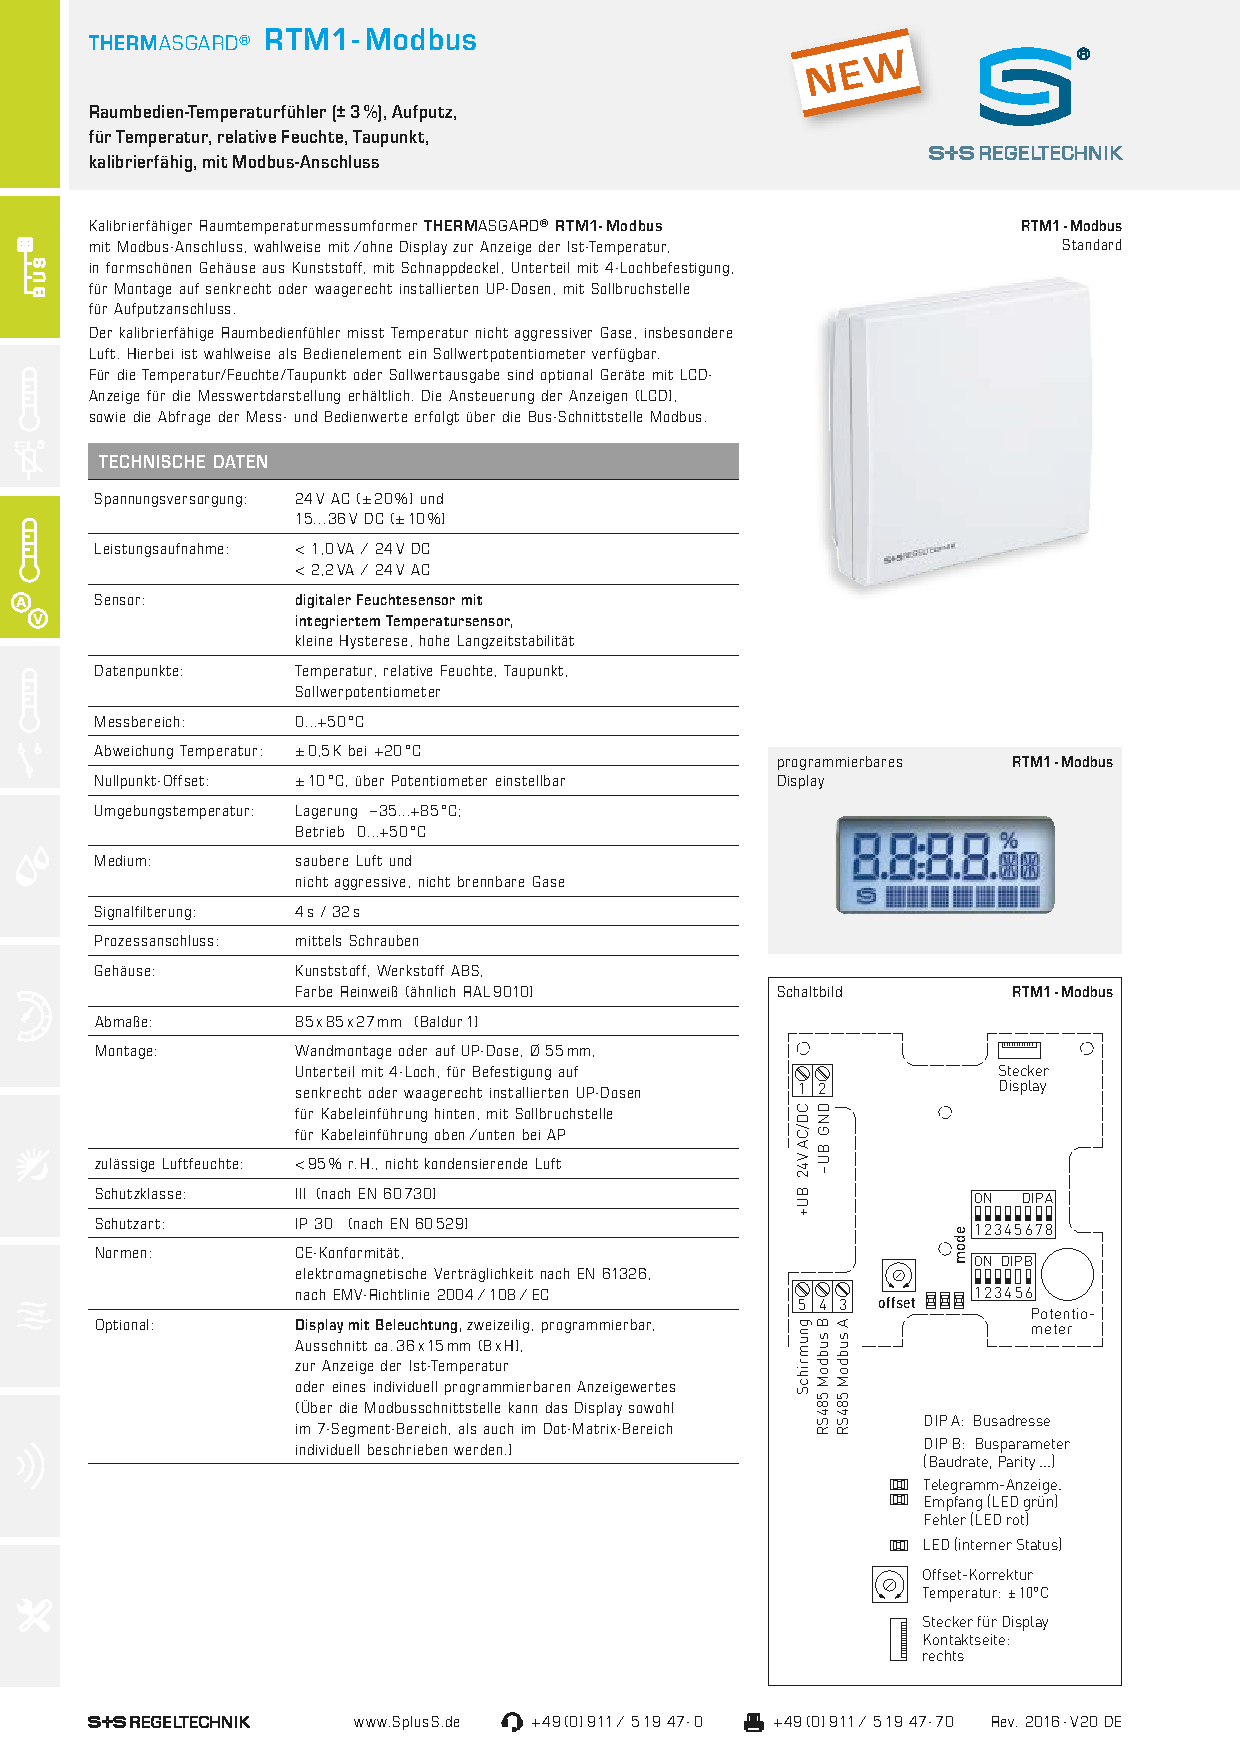
\includepdf[pagecommand={\section{THERMASGARD RTM1-Modbus Raumtemperaturfühler von S+S Regeltechnik}\label{att:rtm1}}, pages={1}, scale=0.7, offset=0.1cm -3cm]{anhang/rtm1}
%\includepdf[pages={2}, scale=0.8]{anhang/rtm1}
%
%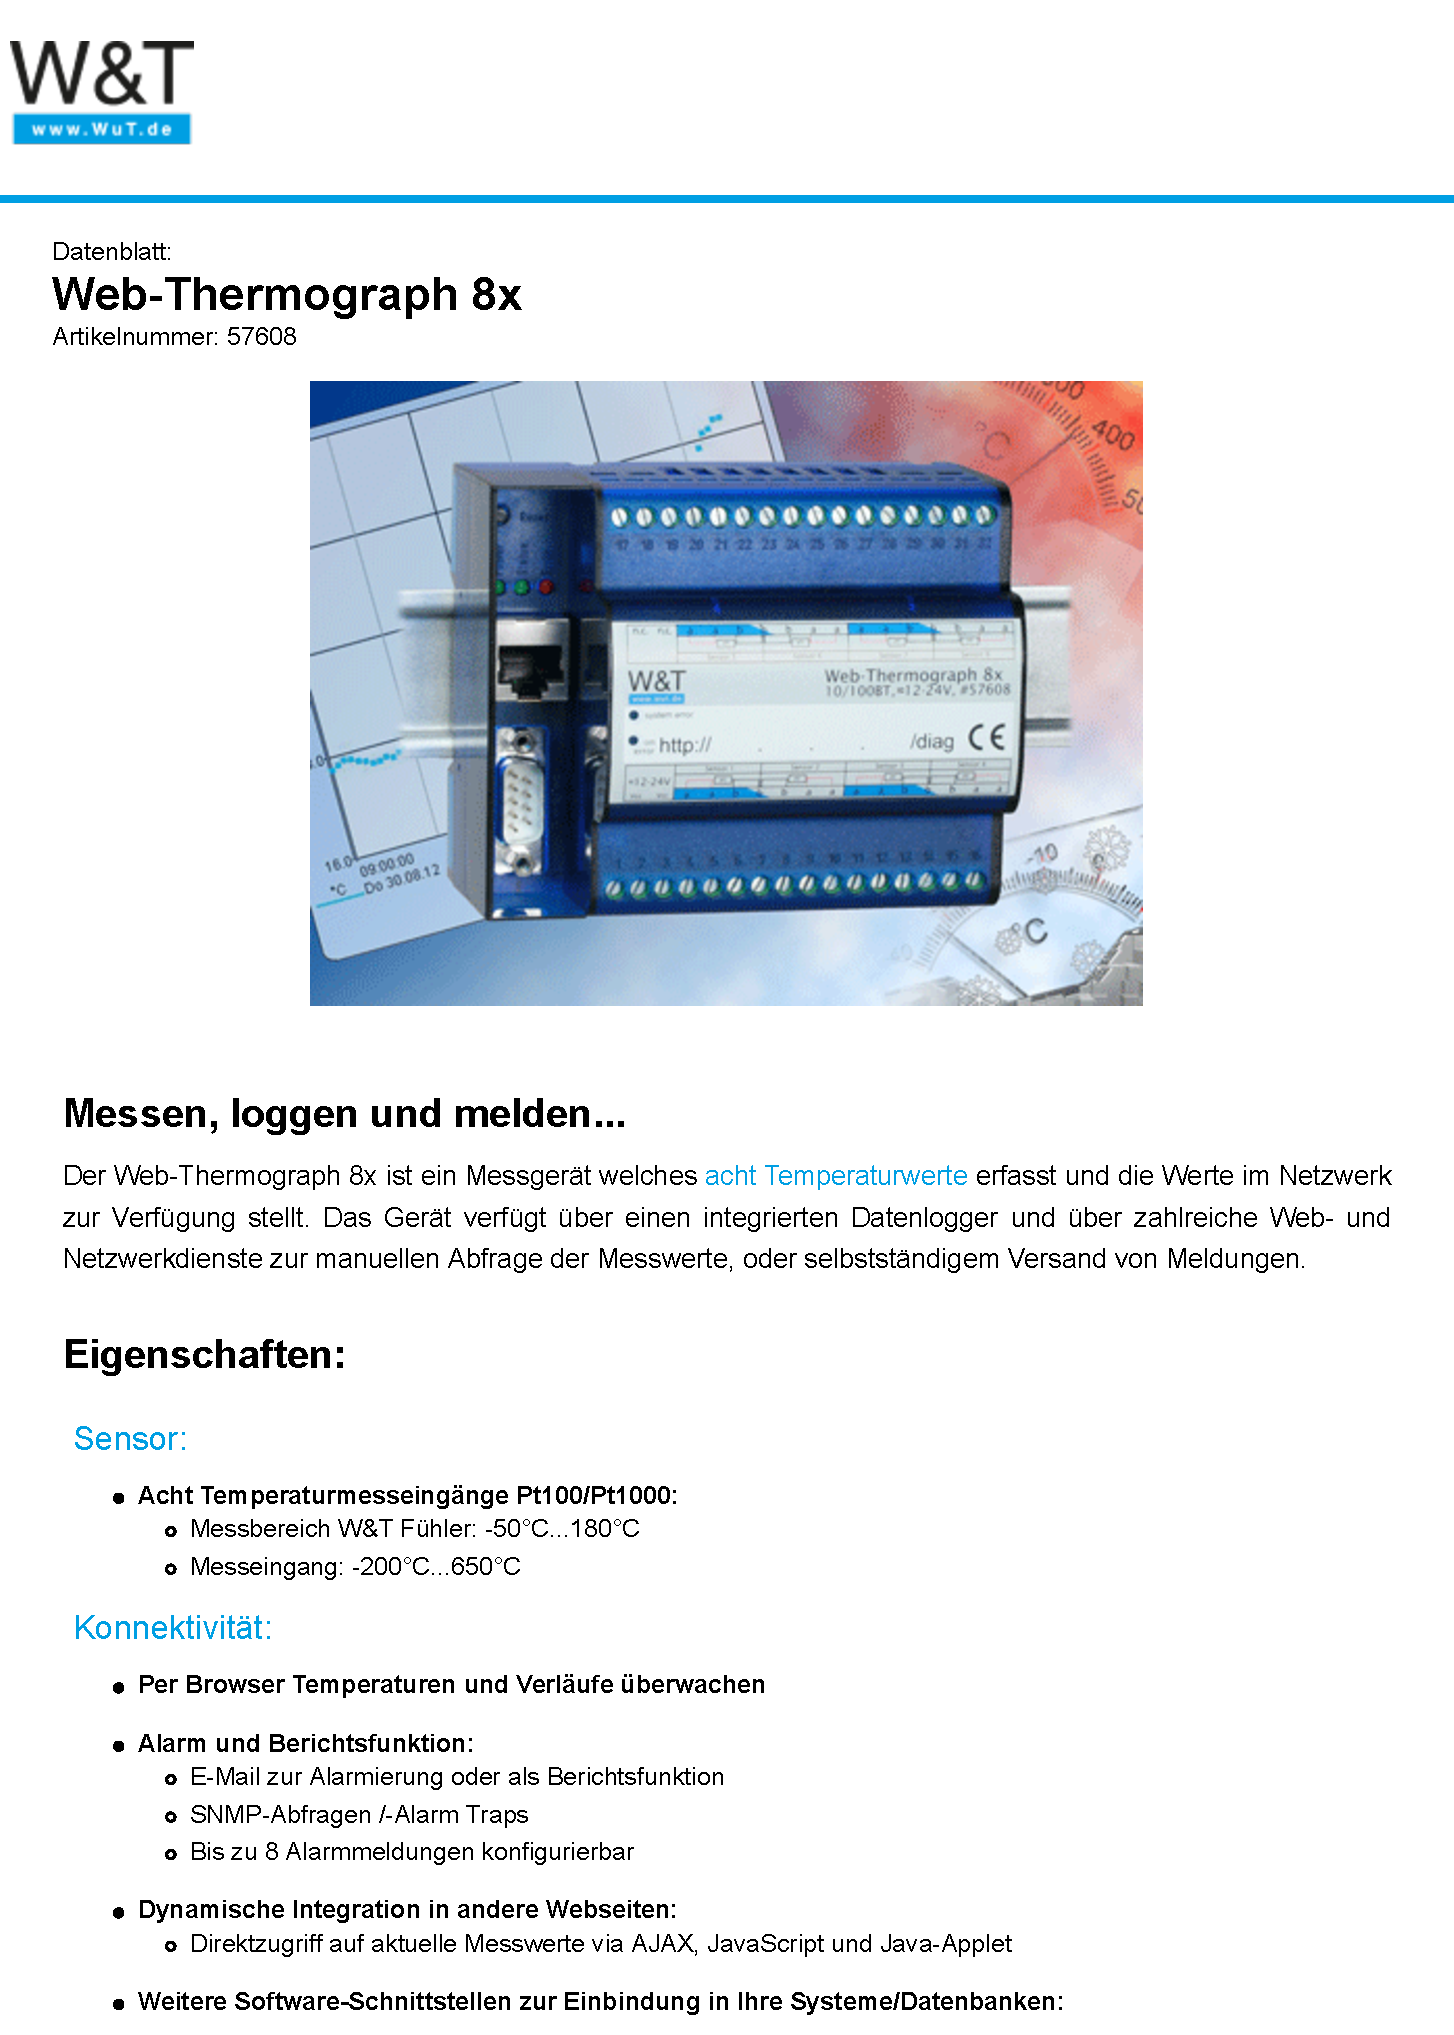
\includepdf[pagecommand={\section{Webthermograph 8x von WuT}\label{att:webtherm}}, pages={1}, scale=0.8, offset=0.1cm -2cm]{anhang/webthermograph8x}
%\includepdf[pages={2-4}, scale=0.8]{anhang/multical}
%
%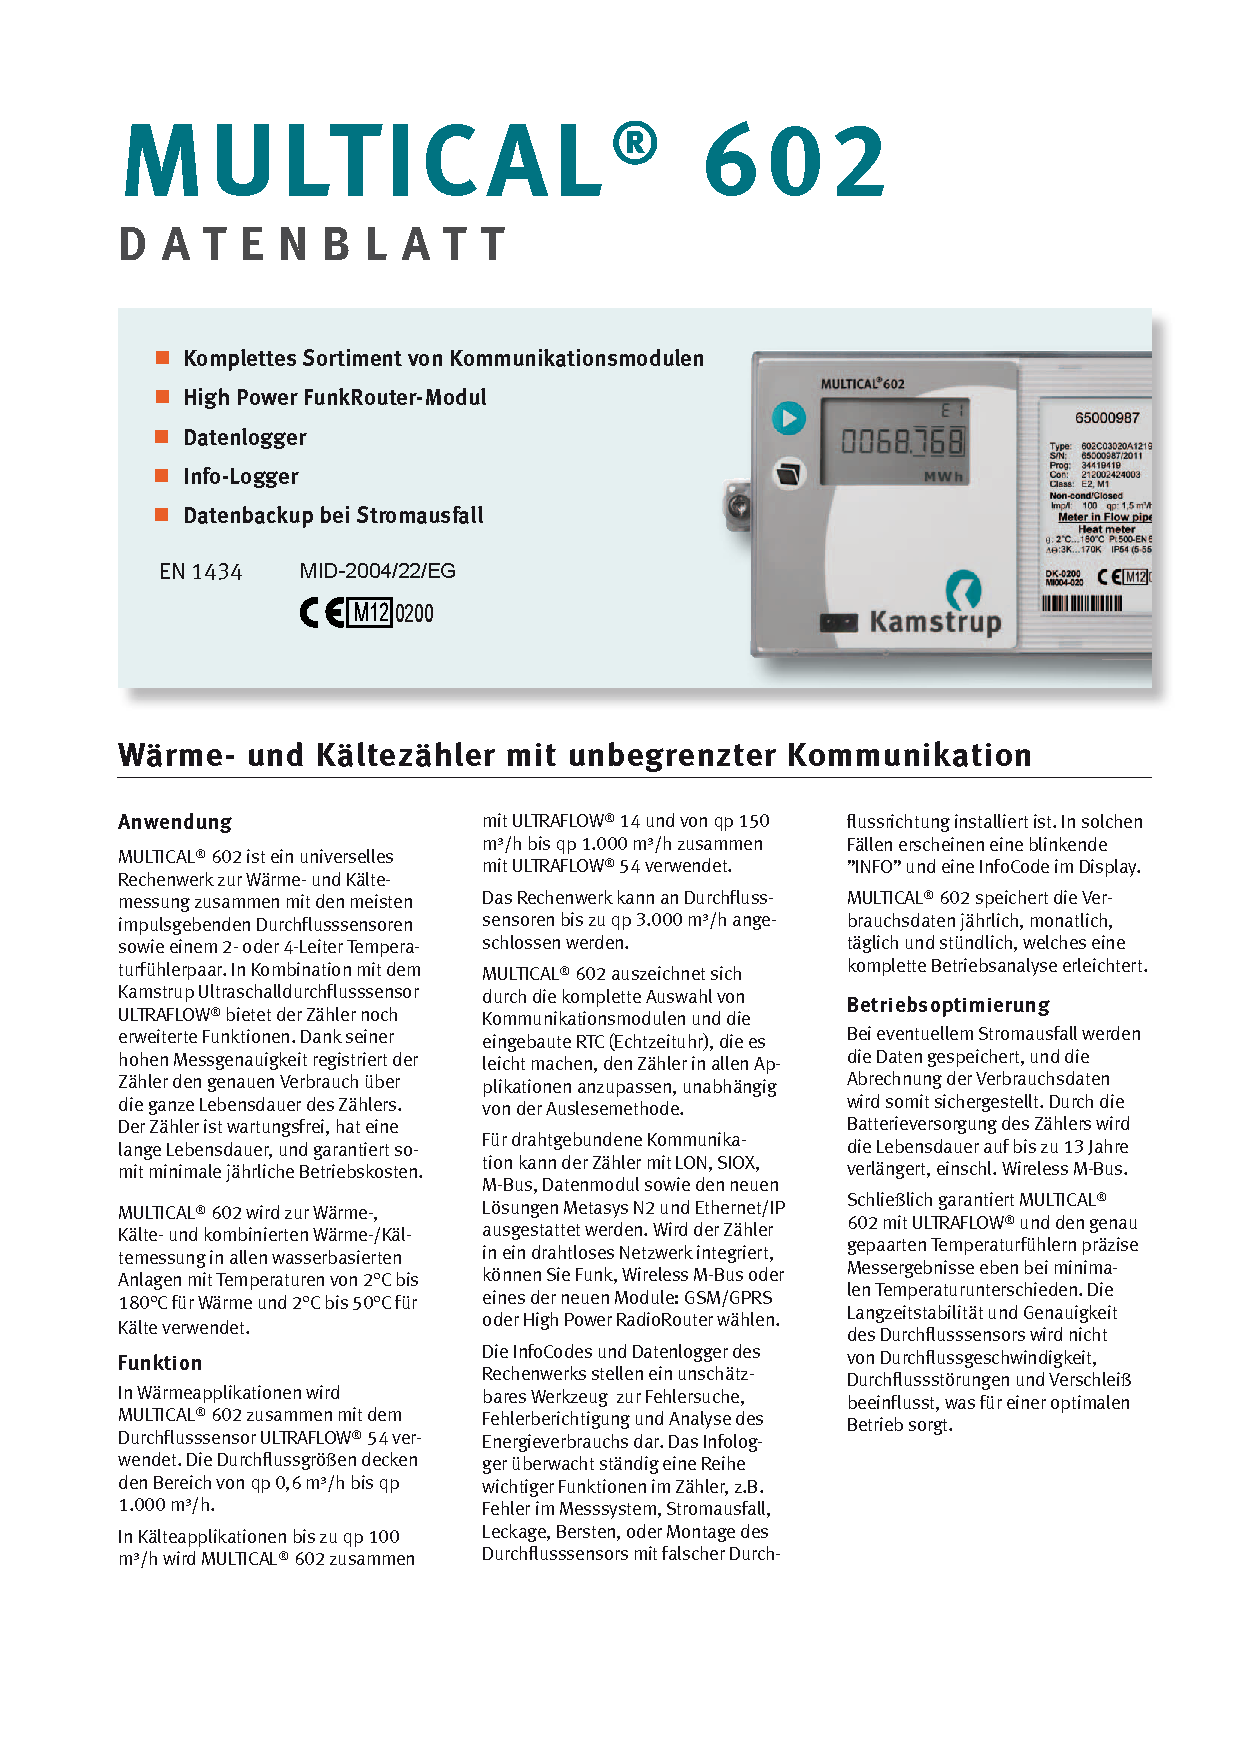
\includepdf[pagecommand={\section{MULTICAL 602 Wärmemengenzähler von Kamstrup}\label{att:multi}}, pages={1}, scale=0.7, offset=0.1cm -2cm]{anhang/multical}
%\includepdf[pages={2}, scale=0.8]{anhang/multical}
%
%
%
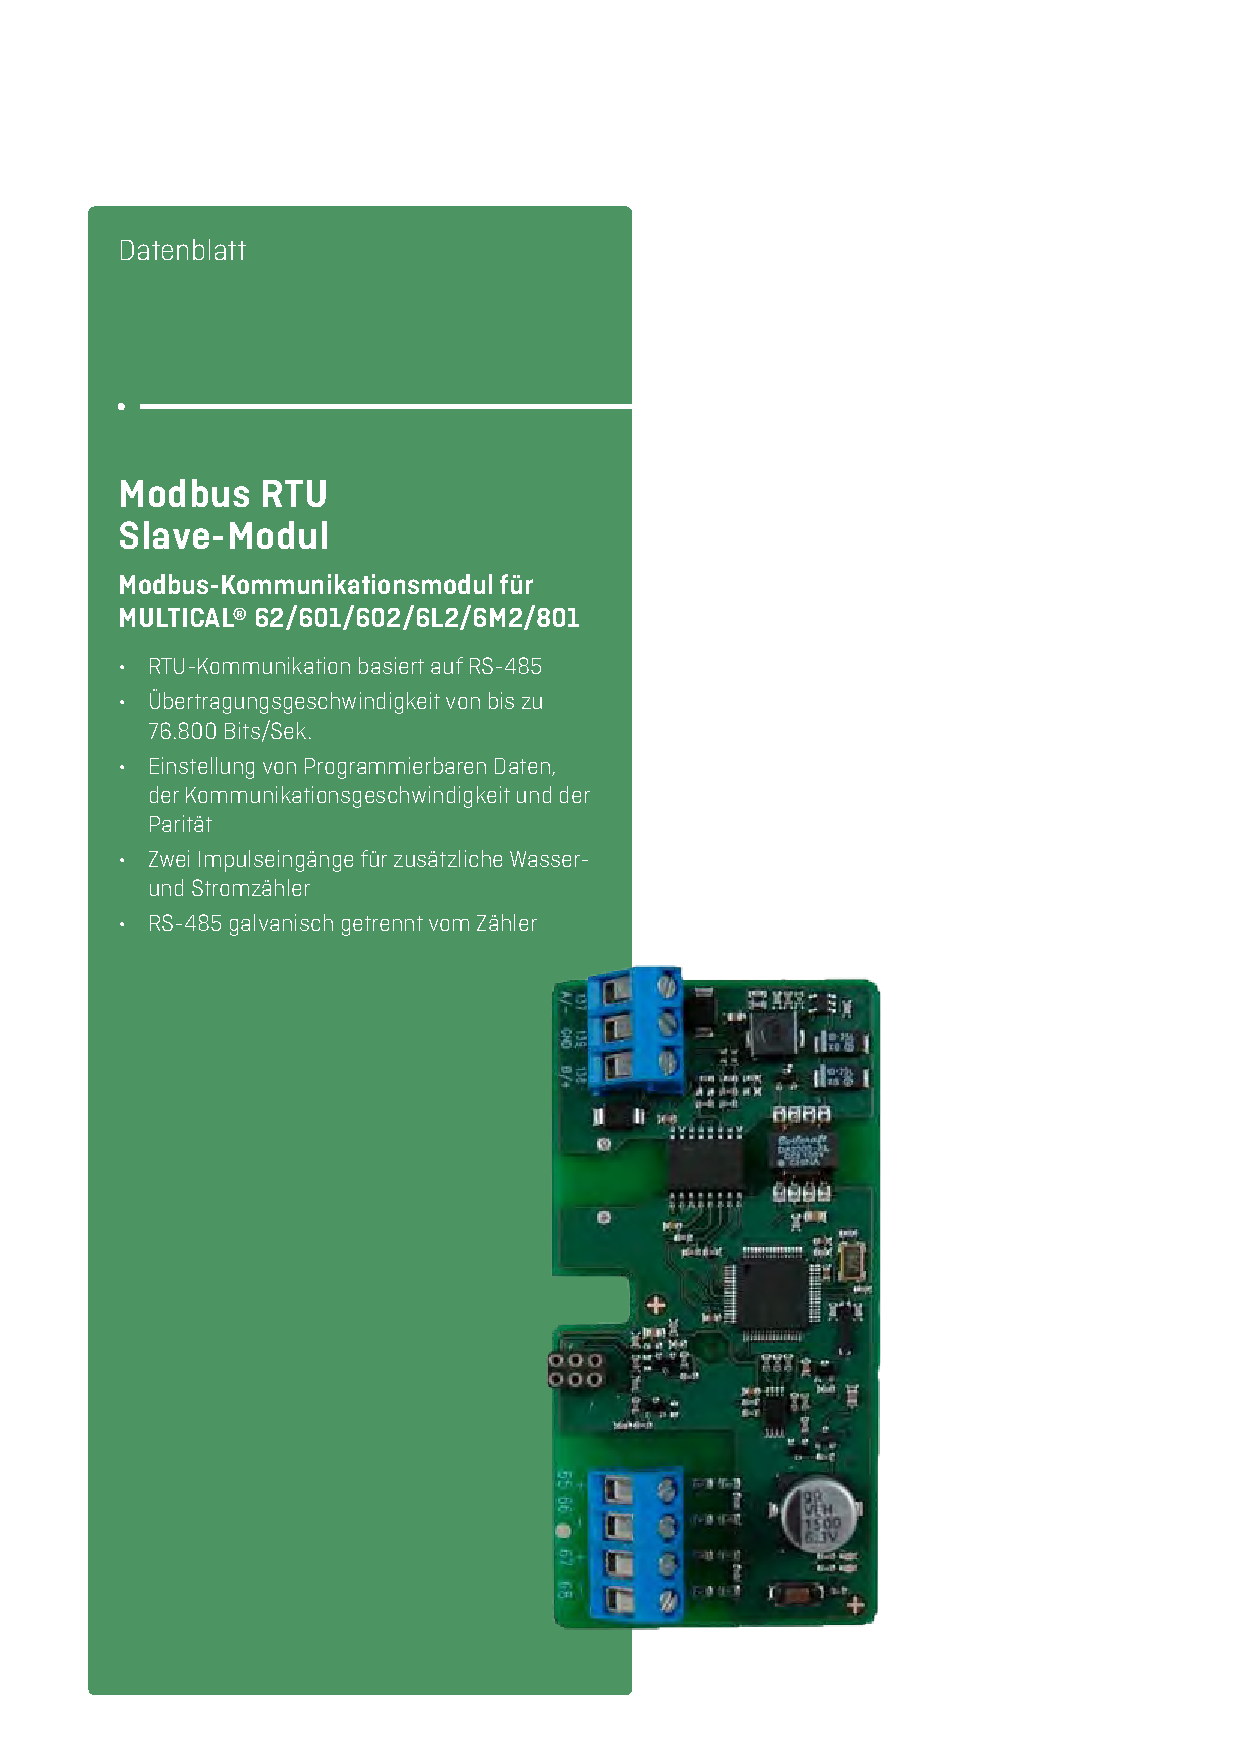
\includepdf[pagecommand={\chapter{Modbusadressmapping}\section{MULTICAL 602 Wärmemengenzähler von Kamstrup}\label{att:modbusmap}}, pages={1}, scale=0.7, offset=0.1cm -2cm]{anhang/multicalmodbus}
%\includepdf[pages={2-7}, scale=0.8]{anhang/multicalmodbus}
%
%\includepdf[pagecommand={\section{THERMASGARD RTM1-Modbus Raumtemperaturfühler von S+S Regeltechnik}\label{att:rtm1modbus}}, pages={4}, scale=0.8, offset=0.1cm -2cm]{anhang/rtmmodbus}
%\includepdf[pages={7-8}, scale=0.8]{anhang/rtmmodbus}
%
%


%\includepdf[pagecommand={\chapter{Datenblätter zum Rückkühlturm}\label{att:daten}\section{Datenblätter SorTech AG zum Rückkühlturm}}, pages={10}, scale=0.7, frame=true, offset=0.1cm -3cm]{attachement/Betriebsanleitung_AdK}
%\includepdf[pages={11-14}, scale=0.8, frame=true]{attachement/Betriebsanleitung_AdK}
%\includepdf[pagecommand={\section{Datenblatt der Wilo-Star Pumpe ST 20/9}\label{att:wilo}}, pages={1}, scale=0.8, frame=true]{attachement/wilo-star-st.pdf}
%\includepdf[pages={4}, scale=0.8, frame=true]{attachement/wilo-star-st.pdf}
%\captionsetup{list=false}                                    % Inhalts-VZ ohne Anhangbilder, aber im Anhang nummeriert

%----------------------------------------------------------------------------------------------------------------------
% Literaturverzeichnis 
%----------------------------------------------------------------------------------------------------------------------
\bibliographystyle{natbib}
\bibliography{quellverz}
\clearpage

%----------------------------------------------------------------------------------------------------------------------
% Eidesstattliche Erklärung 
%----------------------------------------------------------------------------------------------------------------------
%
% Eidesstattliche Erklärung
%
% @version 1.0
% @author wipatrick
% @created 22. November 2015
% @edited 

\chapter*{Eidesstattliche Erklärung}
%\markboth{Eidesstattliche Erklärung}{}
\thispagestyle{empty}
Hiermit erkläre ich, dass ich die vorliegende Arbeit selbstständig und nur unter Benutzung der angegebenen Quellen und Hilfsmittel angefertigt habe. Alle Textstellen, die wörtlich oder sinngemäß aus veröffentlichten oder nicht veröffentlichten Quellen entnommen wurden, sind als solche kenntlich gemacht. Die Arbeit hat in gleicher oder ähnlicher Form keiner anderen Prüfungsbehörde vorgelegen.
 \vspace{2\baselineskip}

\noindent Karlsruhe, den \today
\begin{flushright}
$\overline{~~~~~~~~~\mbox{Daniel Johannes Mayer}~~~~~~~~~}$
\end{flushright}

\end{document}